\documentclass[11pt]{article}
\usepackage[margin=1in]{geometry}
\usepackage{amsmath,amssymb,amsthm,mathtools,microtype,booktabs,array,tikz}
\usepackage[hidelinks]{hyperref}
\usepackage{xurl}
\pdfglyphtounicode{braceex}{23AA}
\pdfglyphtounicode{braceleftBig}{007B FE02}
\pdfglyphtounicode{braceleftBigg}{007B FE04}
\pdfglyphtounicode{braceleftbt}{23A9}
\pdfglyphtounicode{braceleftmid}{23A8}
\pdfglyphtounicode{bracelefttp}{23A7}
\pdfglyphtounicode{bracerightBig}{007D FE02}
\pdfglyphtounicode{bracerightBigg}{007D FE04}
\pdfglyphtounicode{bracketleftBigg}{005B FE04}
\pdfglyphtounicode{bracketleftbigg}{005B FE03}
\pdfglyphtounicode{bracketleftbt}{23A3}
\pdfglyphtounicode{bracketlefttp}{23A1}
\pdfglyphtounicode{bracketrightBigg}{005D FE04}
\pdfglyphtounicode{bracketrightbigg}{005D FE03}
\pdfglyphtounicode{bracketrightbt}{23A6}
\pdfglyphtounicode{bracketrighttp}{23A4}
\pdfglyphtounicode{integraldisplay}{222B FE02}
\pdfglyphtounicode{integraltext}{222B FE01}
\pdfglyphtounicode{mapsto}{21A6}
\pdfglyphtounicode{parenleftBig}{0028 FE02}
\pdfglyphtounicode{parenleftBigg}{0028 FE04}
\pdfglyphtounicode{parenleftbig}{0028 FE01}
\pdfglyphtounicode{parenleftbigg}{0028 FE03}
\pdfglyphtounicode{parenleftbt}{239D}
\pdfglyphtounicode{parenlefttp}{239B}
\pdfglyphtounicode{parenrightBig}{0029 FE02}
\pdfglyphtounicode{parenrightBigg}{0029 FE04}
\pdfglyphtounicode{parenrightbig}{0029 FE01}
\pdfglyphtounicode{parenrightbigg}{0029 FE03}
\pdfglyphtounicode{parenrightbt}{23A0}
\pdfglyphtounicode{parenrighttp}{239E}
\pdfglyphtounicode{productdisplay}{220F FE02}
\pdfglyphtounicode{producttext}{220F FE01}
\pdfglyphtounicode{radicalbig}{221A FE01}
\pdfglyphtounicode{summationdisplay}{2211 FE02}
\pdfglyphtounicode{summationtext}{2211 FE01}
\pdfglyphtounicode{vextendsingle}{20D3}

\AtBeginDocument{%
  \begingroup
  \normalfont\fontencoding{TS1}\selectfont
  \immediate\pdfobj stream {%
/CIDInit /ProcSet findresource begin
12 dict begin
begincmap
/CIDSystemInfo << /Registry (TeX) /Ordering (TS1Bullet) /Supplement 0 >> def
/CMapName /TS1Bullet def
/CMapType 2 def
1 begincodespacerange
<00> <FF>
endcodespacerange
1 beginbfchar
<88> <2022>
endbfchar
endcmap
CMapName currentdict /CMap defineresource pop
end
end
  }%
  \pdffontattr\font{/ToUnicode \the\pdflastobj\space 0 R}%
  \endgroup
}

\hypersetup{pdftitle={Renewal and changes of law for critical honeycomb walks},pdfauthor={OpenAI}}
\newtheorem{theorem}{Theorem}[section]
\newtheorem{proposition}[theorem]{Proposition}
\newtheorem{lemma}[theorem]{Lemma}
\newtheorem{definition}[theorem]{Definition}
\newcommand{\E}{\mathbb E}
\newcommand{\Pp}{\mathbb P}
\newcommand{\one}{\mathbf1}
\DeclareMathOperator{\diam}{diam}
\DeclareMathOperator{\Var}{Var}
\newtheorem{corollary}[theorem]{Corollary}
\newtheorem{remark}[theorem]{Remark}
\newcommand{\Prob}{\mathbb P}
\newcommand{\ind}{\mathbf1}
\newcommand{\R}{\mathbb R}
\newcommand{\N}{\mathbb N}
\newcommand{\Z}{\mathbb Z}
\title{Renewal and changes of law for critical honeycomb walks}
\author{OpenAI}
\date{26 September 2026}
\begin{document}
\maketitle
\begin{abstract}
For critical honeycomb self-avoiding walk, we prove spatial exponent $3/4$ for the infinite irreducible-bridge law and for bridges of every sufficiently large compatible even length. We establish the corresponding thermal laws at every large discount scale, including all positive length and spatial moments. For unrestricted uniform walks, the endpoint lower law holds on a common set of lengths of natural density one. We also determine the near-critical exponential correlation scale and small-force free-energy exponent, and prove spatial local lower bounds that permit conditioning on a prescribed terminal vertex.
\end{abstract}
\tableofcontents
\section{Introduction}
A self-avoiding walk of prescribed length and a self-avoiding walk whose length $L$ is penalized by $e^{-L/N}$ need not have the same distribution in space. The first law fixes one coefficient of a generating function; the second sums all its coefficients, with $N$ setting the discount scale. A third law is obtained by joining independent irreducible bridges forever. Understanding the relations among these laws requires control of their normalizing masses, as well as estimates for the individual paths.

We study these changes of law on the regular honeycomb lattice. Realize its vertices as the centers of the triangles in an equilateral triangular tiling with side length one, and put
\[
 \rho=(2+\sqrt2)^{-1/2}.
\]
A port is the midpoint of a tiling edge on a domain boundary. A strict bridge starts at a prescribed port on one horizontal tiling line, ends at a port on a higher parallel line, and has all its visited vertices strictly between the two lines. A port path with $L$ visited vertices has critical weight $\rho^L$. The ports carry no weight, so adjoining bridges concatenate with exactly the product of their weights. The terminal height and horizontal position are free unless specified.

An intermediate horizontal line crossed exactly once determines a unique cut of a bridge. Cutting at all such lines decomposes the bridge into irreducible bridges. Their critical weights sum to one and therefore define a probability law $p$. Independent $p$-distributed pieces can be concatenated without further avoidance conditions: successive pieces occupy disjoint open slabs. This construction provides the common probability space used throughout the paper.

For an ordinary finite walk $\gamma=(\gamma_0,\ldots,\gamma_n)$, write
\[
 A(\gamma)=|\gamma_n-\gamma_0|,
 \qquad D(\gamma)=\diam\{\gamma_0,\ldots,\gamma_n\}.
\]
Uniform full-plane walks start at one prescribed vertex and have $n$ edges. Uniform half-plane walks start at the inward vertex of a prescribed boundary port and have a prescribed number of visited vertices in the strict half-plane, with their last vertex unrestricted. Thermal walks have variable length and weight $\rho^L e^{-L/N}$, normalized over all such walks. Using edge length instead of vertex length in this last law multiplies all weights by one common factor and gives the same probability measure.

Here are the principal spatial conclusions, with the law included in each statement. The notation $X_t=t^{a+o(1)}$ in probability means that for every $\varepsilon>0$ the event $t^{a-\varepsilon}\le X_t\le t^{a+\varepsilon}$ has probability tending to one.
\begin{itemize}
\item Under the infinite irreducible-bridge law, the distance of the $n$th vertex from the initial port is $n^{3/4+o(1)}$ almost surely, and the number of visited vertices within distance $R$ is $R^{4/3+o(1)}$ almost surely (Theorem~\ref{R:renew:infinite}). Both uniform and fugacity-weighted finite half-plane laws converge on each fixed initial path to this law (Theorem~\ref{R:renew:uniform} and Lemma~\ref{R:renew:halfplane}).
\item Uniform strict bridges with $n$ visited vertices have terminal distance and diameter $n^{3/4+o(1)}$ in probability at every sufficiently large even $n$. The parity restriction is part of the port convention. Critical bridges conditioned instead on height $h$ have length $h^{4/3+o(1)}$ in probability (Theorems~\ref{R:exact:bridge} and~\ref{R:exact:height}).
\item Uniform endpoint-free half-plane and full-plane walks have endpoint distance and diameter $n^{3/4+o(1)}$ in probability along a common set of lengths of natural density one. Their upper spatial bound holds at every sufficiently large length, with arbitrarily high polynomial accuracy (Theorems~\ref{R:cal:halfplane-laws} and~\ref{R:cal:plane-laws}).
\item For thermal half-plane and full-plane walks, $L=N^{1+o(1)}$ and $A,D=N^{3/4+o(1)}$ in probability. Their positive moments have the corresponding exponents: for each fixed $p>0$, $\E L^p=N^{p+o(1)}$ and $\E A^p,\E D^p=N^{3p/4+o(1)}$ (Theorems~\ref{R:thermal:law} and~\ref{R:cal:halfplane-laws}).
\end{itemize}
The full-plane endpoint lower bound at fixed length retains the density-one qualification. The thermal statement concerns every large discount scale $N$. These conclusions use different normalization arguments, described below. Nienhuis's analysis of the two-dimensional $O(n)$ model predicts the spatial exponent $\nu=3/4$ for self-avoiding walk in the $n\to0$ polymer limit~\cite[Eqs.~(1)--(2)]{Nienhuis1982}; the results here retain the sampling-law and length qualifications stated above.

\subsection*{Bridge theory and the additional estimates}
Kesten's normalization for irreducible bridges underlies the infinite-bridge construction of Madras and Slade~\cite{Kesten1963,MadrasSlade1993}. Lawler, Schramm and Werner identify this measure as the fixed-length half-space limit and describe its fugacity counterpart~\cite[Appendix]{LSW2004}. Dyhr, Gilbert, Kennedy, Lawler and Passon give explicit finite-prefix descriptions of both limits and identify the strip law by conditioning on a renewal height~\cite[Propositions~2.2--2.3, 2.9 and~2.10]{Dyhr2011}. These works use vertex conventions on the integer lattice; the strip construction of Dyhr et al. also includes a final bond from the conditioning height to the target height. We adapt the renewal arguments to the present honeycomb port convention and prove the required normalizations here. The infinite law, a fixed-height bridge law and a law conditioned on one exact length are different uses of the construction.

Duminil-Copin and Smirnov proved the value of $\rho$ using a parafermionic observable on the honeycomb lattice~\cite{DCS2012}. Beaton et al. use a honeycomb mid-edge renewal construction and prove that the critical bridge mass tends to zero as the strip height grows~\cite[Theorem~10 and Appendix]{BeatonEtAl2014}. Krachun and Panagiotis obtain a positive-power decay bound for this mass and show that a uniform $n$-step honeycomb walk remains within distance $O(n/\log n)$ of its root with probability tending to one~\cite{KrachunPanagiotis2026}.

The sharper finite estimates used below require additional strip and marked-polygon arguments. We state the companion results as estimates of positive walk weights. In Section~\ref{R:sec:renewal}, the finite bridge estimates of Theorem~\ref{R:renew:finite-input} and the renewal identities yield joint bounds for the height, length and diameter of one irreducible. Section~\ref{R:geo:section} uses further finite strip and polygon estimates to control avoidance and absolute path masses. The analytic finite estimates are proved in the cited companions; the present paper proves the renewal and geometric transfers needed when the sampling law changes.

The key exponents for one irreducible are
\[
 \alpha=\frac9{16},\qquad \beta=\frac34.
\]
Write $H,L,D$ for the height, vertex length and diameter of one irreducible. On the main route the finite estimates give
\[
 1-\E_p e^{-uL}\asymp u^\alpha,\qquad
 1-\E_p e^{-sH}\asymp s^\beta,\qquad
 \Pp_p\{D>r\}\le Cr^{-\beta}
\]
as $u,s\downarrow0$ and $r\to\infty$. Here $\asymp$ means upper and lower bounds with positive constants independent of the parameter. The ratio $\alpha/\beta=3/4$ explains the spatial scale after many pieces have been joined. Turning this observation into a theorem at one exact length requires more than a sum estimate.

\subsection*{How the normalizations are controlled}
Our main exact-length route uses these bounded-factor finite estimates. If $S_L(k)=L_1+\cdots+L_k$ for independent irreducibles, the local denominator is
\[
 u_n=\Pp_p\{S_L(k)=n\text{ for some }k\}\ge c n^{\alpha-1}
 \quad\text{for all sufficiently large even }n.
\]
Section~\ref{R:sec:exact} proves this by exponential tilting and Fourier inversion on the compatible length lattice. Fourier concentration for the remaining pieces then pays for sequences with atypical total height or diameter. The identification of the uniform half-plane prefix limit in Section~\ref{R:sec:renewal} is a separate ratio argument.

A second, self-contained route begins with a logarithmic window of bridge lengths. Its length information is weaker:
\[
 c u^\alpha(\log(1/u))^{-P}\le 1-\E_p e^{-uL}\le C u^\alpha.
\]
A Fourier difference estimate first gives a long interval on which the renewal mass has the required lower bound. Fresh independent increments then move the remaining length into that interval. The logarithmic window permits enough progress at each stage that the total landing cost is only $n^{-o(1)}$, giving $u_n\ge n^{\alpha-1-o(1)}$. Section~\ref{R:cal:section} proves this alternative under its own hypotheses, with a fixed logarithmic exponent below one and a stopping interval whose width remains large.

Section~\ref{R:geo:section} next establishes the geometric estimates used in the thermal transfer of Section~\ref{R:sec:thermal}. A half-plane walk consists of a list of complete irreducibles followed by a remainder with no further renewal. In a prescribed-prefix probability, the total weight of that remainder cancels exactly. For an unrestricted plane walk we obtain a denominator by putting a nonempty bridge between two exterior remainders. Recovering the first and last single-crossing lines makes this construction injective. To bound small endpoint displacement, we cut a path at its lowest vertex and use the two-end estimate of Corollary~\ref{R:geo:two-ends}, retaining one independent height-smoothing variable. The two remainder weights then appear in both numerator and denominator and cancel.

The censored-arm estimates in Section~\ref{R:cal:geometry-section} give a separate geometric route from the logarithmic finite inputs to absolute spatial bounds. Section~\ref{R:cal:uniform-section} then treats moments and uniform walks, where there is no comparable exact cancellation at each length. In the half-plane, disjoint long-prefix events compare masses at nearby lengths. In the full plane, we insert a bridge at a minimum and use censored survival to control the inverse multiplicity. Both arguments average logarithms of the nearby-length masses: the interior terms telescope and leave a boundary error. This is why the resulting lower laws hold on a density-one set.

Next, let $G_t(b)$ be the total weight $(\rho e^{-t})^{\ell(\gamma)}$ of ordinary walks from a fixed vertex $o$ to $b$, with edge length $\ell$. Section~\ref{R:resp:section} proves that the convergence threshold in $s$ of
$\sum_bG_t(b)e^{s e\cdot(b-o)}$ is $t^{3/4+o(1)}$, uniformly for unit directions $e$. The fixed-length free energy
\[
 f_e(s)=\lim_{j\to\infty}\frac1j\log\sum_{\ell(\gamma)=j}\rho^j e^{s e\cdot(\gamma_j-o)}
\]
exists and is $s^{4/3+o(1)}$ as $s\downarrow0$, uniformly in $e$. Its two one-sided derivatives are $s^{1/3+o(1)}$, in agreement with Pincus's force-extension scaling relation $1/\nu-1$ at $\nu=3/4$~\cite[Eq.~(I.4)]{Pincus1976}. Here the response follows from the threshold bounds and convexity; the distinction from fixed-force ballistic results is discussed in Section~\ref{R:resp:section}.

Prescribing a terminal vertex requires a further estimate: if $|b_N-o|=N^{3/4+o(1)}$, the thermal law conditioned to end at $b_N$ has length $N^{1+o(1)}$ and diameter $N^{3/4+o(1)}$ in probability, with the corresponding powers for all positive moments (Theorem~\ref{R:resp:prescribed}). Proposition~\ref{R:resp:point-local} obtains a uniform two-dimensional lattice lower bound from subsequential local limits. A lower partition bound supported in a corridor then permits this conditioning. The separate spatial-rate statement takes distance to infinity at fixed discount and then takes the discount to zero; it does not identify these two orders of limits.

The final three sections develop consequences of other finite inputs. Section~\ref{R:alt:section} retains a length reward in a logarithmically enlarged box and a completed-prefix expectation in a fixed-proportion ball. Section~\ref{R:alt:j} derives the irreducible length tail from signed cylinder and marked-polygon estimates. Section~\ref{R:alt:g:section} gives a geometric route to the infinite and thermal laws, using future-renewal averaging for the infinite path and recoverable tall-bridge insertion for the thermal path. These routes state their own finite inputs and retain the precision those inputs supply.

\section{One probability space for the different laws}\label{R:sec:renewal}
The elementary renewal identities must precede the changes of measure. They concern complete irreducible pieces. In particular, no independence between the length, height and displacement of one piece is assumed.

\subsection{Ports, strips and the finite input}
Fix one port on a horizontal row boundary. A strict bridge of height $h\in\N$ has its other port on the boundary $h$ rows above and all its vertices in the open strip between these boundaries. One row has Euclidean height $d_0=\sqrt3/2$. Write $\mathcal B_h$ for this set, with the terminal port unrestricted, and set
\[
 B_h=\sum_{\gamma\in\mathcal B_h}\rho^{L(\gamma)},\qquad
 M_h=\sum_{\gamma\in\mathcal B_h}L(\gamma)\rho^{L(\gamma)},\qquad B_0=1.
\]
The term at height zero denotes an empty concatenation, not a nonempty walk. For every port path its diameter includes both ports as well as its visited vertices. Heights and transverse displacements use the actual staggered honeycomb port lattice. All paths and all translations below retain their starting port; there is never an extra sum over its position.

Here is the positive finite input for our main route. Its proof belongs to the uniform marked-polygon calculation and its exterior sewing argument.
\begin{theorem}[Finite bridge estimates]\label{R:renew:finite-input}
There are constants $c,C>0$ such that, for every sufficiently large integer $h$,
\[
 c h^{-1/4}\le B_h\le C h^{-1/4},\qquad M_h\le C h^{13/12},\qquad
 B_h\{L\ge c h^{4/3}\}\ge c h^{-1/4}.
\]
For all $h\ge1$ and $x\ge1$, one also has
\[
 B_h\{D>x\}\le C x^{-1/4}.
\]
The same estimates hold in the symmetry-related pure directions.
\end{theorem}
These are the bounded-factor estimates of \cite[Theorem~1.1]{companionU}. All finitely many smaller-height masses and first moments are finite as well: append a fixed straight bridge to inject their paths into a sufficiently tall strip, with bounded weight and additive length changes. We enlarge constants to include these heights. The first moment and the positive mass of long bridges play different roles: the former bounds a truncated irreducible reward, whereas the latter supplies a lower length deficit. Exponent-only versions lead to the weaker, explicitly stated variants later in the paper.

\subsection{Factorization and marked rewards}
An intermediate row boundary crossed exactly once is a renewal boundary. Cutting a strict bridge at every renewal boundary gives an ordered list of irreducible bridges, each of positive integral height. Conversely, a list of irreducibles concatenates to a strict bridge: its pieces occupy disjoint open strips. Let $\mathcal I$ be the set of irreducibles rooted at our fixed port and initially put $p(\gamma)=\rho^{L(\gamma)}$.

\begin{proposition}[Renewal factorization]\label{R:renew:factorization}
The masses $p(\gamma)$ sum to one. If $H,L,X,D$ denote respectively the height, visited-vertex length, signed transverse displacement and Euclidean diameter of an irreducible, then, for $s>0$ and $u\ge0$,
\[
 b(s,u):=\sum_{h\ge0}\sum_{\gamma\in\mathcal B_h}
       \rho^{L(\gamma)}e^{-sh-uL(\gamma)}
 =\frac1{1-\E_p e^{-sH-uL}}.
\]
In particular $b(s,0)\asymp s^{-3/4}$ as $s\downarrow0$. Under independent successive samples from $p$, $B_h$ is the probability that some renewal occurs at height $h$.
\end{proposition}
\begin{proof}
Unique factorization and multiplication of vertex weights give the geometric series with nonnegative terms. The finite strip estimate makes $b(s,0)$ finite for $s>0$, so $\sum p(\gamma)e^{-sH(\gamma)}<1$. Monotone convergence as $s\downarrow0$ gives $\sum p\le1$. On the other hand, summing $B_h\asymp(1+h)^{-1/4}$ gives $b(s,0)\asymp s^{-3/4}\to\infty$, forcing $\sum p=1$. Positive heights make the events that the $k$th renewal has height $h$ disjoint as $k$ varies. Summing their probabilities yields the last assertion.
\end{proof}

For a nonnegative function $f$ of an irreducible, define the height-indexed reward
\[
 p_f(j)=\E_p[f;H=j],\qquad
 B_f(h)=\sum_{\gamma\in\mathcal B_h}\rho^{L(\gamma)}
                 \sum_{I\text{ a piece of }\gamma} f(I).
\]
\begin{lemma}[Additive rewards]\label{R:renew:reward}
With convolution on nonnegative integral heights,
\[
 B_f=B*p_f*B,\qquad
 \sum_h e^{-sh}B_f(h)=b(s,0)^2\E_p[fe^{-sH}].
\]
These identities hold as identities of nonnegative sums, even when a sum is infinite. For $f=L$, $B_f(h)=M_h$.
\end{lemma}
\begin{proof}
Mark one piece in a bridge and then cut immediately before and after it. The pieces before the mark form an arbitrary bridge, the mark is one irreducible, and the pieces after it form another arbitrary bridge. This is a bijection, with multiplicative weights. Tonelli's theorem gives both formulas. Since length is additive across ports, summing the lengths of all pieces gives the full visited-vertex length.
\end{proof}

\subsection{Joint increment estimates}
The next statement concerns the joint law of the four coordinates, rather than four independent variables. Its exponent-only consequences are sufficient for the prescribed-endpoint applications.
\begin{proposition}\label{R:renew:increments}
Put $\beta=3/4$ and $\alpha=9/16$. Under $p$,
\begin{align*}
 1-\E_p e^{-sH}&\asymp s^\beta,&
 p(H>x)+p(D>x)&\le Cx^{-\beta},\\
 \E_p[L;H\le x]&\le Cx^{7/12},&
 p(L>n)&\le Cn^{-\alpha},&
 1-\E_p e^{-uL}&\asymp u^\alpha.
\end{align*}
The constants are uniform for sufficiently small positive $s,u$ and sufficiently large $x,n$.
\end{proposition}
\begin{proof}
The first assertion follows directly from Proposition~\ref{R:renew:factorization}. Since $1-e^{-H/x}\ge1-e^{-1}$ on $H>x$, it gives the height tail.

We first prove the diameter tail, which is not a consequence of the height tail alone. Set $s=A/x$ with a fixed large $A$. Give all finite bridges their normalized weight proportional to $\rho^L e^{-sH}$; its normalizer is $b(s,0)$. The mass of bridges of diameter greater than $x$ is at most
\[
 Cx^{-1/4}\sum_{h\ge1}e^{-sh}\le Cx^{-1/4}s^{-1}.
\]
Relative to $b(s,0)\ge c s^{-3/4}$ this is at most $C A^{-1/4}$. Choose $A$ so that this is at most $1/2$. Put $q=\E_p[e^{-sH};D>x]$ and $d=1-\E_p e^{-sH}$. The relative mass of bridge lists containing at least one such piece is exactly
\[
 1-\frac{d}{d+q}=\frac{q}{d+q}.
\]
A piece of diameter greater than $x$ forces the whole bridge to have that diameter. Thus $q\le d\le C_Ax^{-3/4}$. On $H\le x$, $e^{-sH}\ge e^{-A}$; on $H>x$ use the height tail. This proves $p(D>x)\le Cx^{-3/4}$.

For the reward bound, retain in Lemma~\ref{R:renew:reward} only the marked pieces of height at most $x$ and outer bridges of heights at most $x$. Their total height is at most $3x$, whence
\[
 \left(\sum_{h\le x}B_h\right)^2\E_p[L;H\le x]
 \le\sum_{h\le3x}M_h\le Cx^{25/12}.
\]
Since the squared factor on the left is at least $cx^{3/2}$, the reward is at most $Cx^{7/12}$. Taking $x=n^{3/4}$ and splitting according to $H>x$ gives
\[
 p(L>n)\le p(H>x)+n^{-1}\E_p[L;H\le x]
 \le Cn^{-9/16}.
\]
Integration of this tail yields $\E_p(1-e^{-uL})\le Cu^{9/16}$.

For the reverse bound take $s=R^{-1}$ and $u=R^{-4/3}$. On every height $R\le h\le2R$, Theorem~\ref{R:renew:finite-input} retains critical mass at least $cR^{-1/4}$ with $L\ge cR^{4/3}$. Consequently
\[
 b(s,0)-b(s,u)\ge cR^{3/4}\ge c' b(s,0).
\]
Writing $d_s=1-\E_p e^{-sH}$ and
$e_{s,u}=\E_p[e^{-sH}(1-e^{-uL})]$, the renewal identity makes the relative difference equal to $e_{s,u}/(d_s+e_{s,u})$. The displayed lower bound therefore implies $e_{s,u}\ge c d_s\ge cR^{-3/4}$. Finally $\E_p(1-e^{-uL})\ge e_{s,u}$ and $R^{-3/4}=u^{9/16}$.
\end{proof}

\begin{remark}\label{R:renew:weak-scope}
If the first-length upper bound and the mass of long bridges have only exponent precision, the same proof gives
\[
 \E_p[L;H\le x]\le x^{7/12+o(1)},\quad
 p(L>n)\le n^{-9/16+o(1)},\quad
 1-\E_p e^{-uL}=u^{9/16+o(1)}.
\]
The bounded-factor height and diameter tails are unchanged. These are the joint-law inputs used in the prescribed-endpoint arguments of Section~\ref{R:resp:section}; no endpoint conditioning is implicit in them.
\end{remark}

\subsection{Infinite concatenation and spatial growth}
We record once the elementary conversion from a Laplace deficit to the growth of independent sums.
\begin{lemma}\label{R:renew:growth}
Let $Y_1,Y_2,\ldots$ be independent copies of a nonnegative random variable $Y$, and let $0<a<1$. If $\Prob(Y>t)\le t^{-a+o(1)}$, then almost surely
$\sum_{j\le k}Y_j\le k^{1/a+o(1)}$. If also
$1-\E e^{-uY}=u^{a+o(1)}$, then almost surely
$\sum_{j\le k}Y_j=k^{1/a+o(1)}$.
\end{lemma}
\begin{proof}
Fix $\epsilon>0$ and let $k=2^j$. Put $t=k^{1/a+\epsilon}$. The probability of a summand above $t$ is at most $k t^{-a+o(1)}$. Moreover
$\E[Y\ind_{Y\le t}]\le t^{1-a+o(1)}$, by integrating the tail, so Markov's inequality bounds the probability that the truncated sum exceeds $t$ by the same expression. This is a summable geometric sequence in $j$. For the lower bound put $t=k^{1/a-\epsilon}$ and $u=t^{-1}$. Exponential Markov gives
\[
 \Prob\{\textstyle\sum_{i\le k}Y_i\le t\}
 \le e\big(\E e^{-Y/t}\big)^k
 \le\exp\{1-k t^{-a+o(1)}\},
\]
also summable. Borel--Cantelli, monotonicity between consecutive dyadic $k$, and a countable sequence of $\epsilon\downarrow0$ prove the claims.
\end{proof}

\begin{theorem}[Infinite spatial law]\label{R:renew:infinite}
Concatenate independent irreducibles of law $p$, and enumerate the resulting vertices as $\gamma_1,\gamma_2,\ldots$. Almost surely,
\[
 |\gamma_n-\gamma_1|=n^{3/4+o(1)},\qquad
 \#\{n:|\gamma_n-\gamma_1|\le R\}=R^{4/3+o(1)}.
\]
\end{theorem}
\begin{proof}
Lemma~\ref{R:renew:growth} and Proposition~\ref{R:renew:increments} give
\[
 \sum_{i\le k}L_i=k^{16/9+o(1)},\qquad
 \sum_{i\le k}H_i=k^{4/3+o(1)},\qquad
 \sum_{i\le k}D_i\le k^{4/3+o(1)}
\]
on one event of probability one. If vertex $n$ lies in piece $k+1$, it is above the last completed renewal boundary and within the total diameter of the first $k+1$ pieces. The first of the three bounds implies $k=n^{9/16+o(1)}$: both consecutive partial sums have the same exponent, so an exceptionally long current piece creates no missing interpolation interval. The height lower bound and diameter upper bound give the first conclusion. For each fixed $\epsilon>0$, all sufficiently large $n$ then obey $n^{3/4-\epsilon}\le |\gamma_n-\gamma_1|\le n^{3/4+\epsilon}$. Inverting these two inequalities gives the asserted count of vertices in a ball.
\end{proof}

\subsection{Uniform half-plane paths have the same prefix limit}
The fugacity cancellation will follow directly from factorization in Section~\ref{R:sec:thermal}. Uniform paths of one exact length require a separate ratio argument. The passage from a two-step counting ratio to the prefix limit adapts the argument of Lawler, Schramm and Werner~\cite[Appendix]{LSW2004} and Dyhr et al.~\cite[Section~2.3, Proposition~2.9]{Dyhr2011} to honeycomb ports; we prove the required ratio by local hexagon flips. Let $a_n$ count paths of $n$ visited vertices starting inward from our bottom port and otherwise unrestricted in the strict upper half-plane; put $a_0=1$.
\begin{theorem}\label{R:renew:uniform}
One has $a_{n+2}/a_n\to\rho^{-2}$. The uniform half-plane laws converge on each fixed initial path to the infinite law of Theorem~\ref{R:renew:infinite}.
\end{theorem}
\begin{proof}
First $a_n^{1/n}\to\rho^{-1}$. The upper bound is the honeycomb connective-constant theorem \cite{DCS2012}. For the lower bound, let $b_m$ count strict bridges of length $2m$ over all heights. Concatenation at a prescribed length is injective, so $b_{m+j}\ge b_mb_j$; also $b_1>0$. The divergence $\sum_m b_m\rho^{2m}=\sum_hB_h=\infty$ and supermultiplicativity imply the required root bound along even lengths. Length-two bridges fill the bounded remainders after repeating a fixed long block. Extending the terminal port by one vertex gives the odd-length bound.

A path is specified, up to bounded initial choices, by its left/right turn word. Runs have length at most four, since five equal turns close an elementary hexagon. Except for an exponentially negligible fraction at length $n$, there are at least $\delta n$ maximal runs of length three, for some fixed $\delta>0$. Indeed, compositions into parts $1,2,4$ have growth less than $\rho^{-1}$ because $\rho+\rho^2+\rho^4<1$. Assign a sufficiently small positive weight $v<1$ to every part of length three. The geometric composition series still has growth at most $\lambda<\rho^{-1}$; the words with at most $\delta n$ such parts number at most $C(v^{-\delta}\lambda)^n$. Choose $\delta$ small enough and use the root bound above.

Such a run follows a four-edge arc of a hexagonal face, with exterior entrance and exit edges. The one omitted face vertex cannot be used internally elsewhere, because two of its neighbors are already saturated. Discard faces incident to either endpoint and the bounded number of runs at the ends of the word. The remaining faces are wholly in the strict half-plane: a honeycomb face intersecting its boundary has at most three vertices strictly above it. Each retained four-edge arc may therefore be replaced by the complementary two-edge arc.

Call a wholly allowed face a slot if it avoids the endpoints, is traversed in one consecutive two- or four-edge arc using exterior entrance and exit edges, and has all its remaining vertices unused. A flip changes the length by two. Color faces with finitely many colors so that faces of one color have disjoint vertex sets. For a fixed color the slot set is unchanged by its flips. Each resulting equivalence class with $k$ slots has $\binom{k}{j}$ paths of lengths $n_0+2j$, where $j$ is the number of four-edge arcs.

Put $\theta=\rho^2/(1+\rho^2)$. For each color and each fixed $\epsilon>0$, paths of length $n$ for which $k\ge\epsilon n$ but $|j/k-\theta|\ge\epsilon$ have exponentially negligible proportion. To see this, weight every path by $\rho^{\text{length}}$. In each class shift $j$ towards $k\theta$ by $\lfloor\eta n\rfloor$ steps, with a sufficiently small fixed $\eta>0$, using the same sign for each of the two deviation classes. The binomial successive ratios show that the new weighted class count exceeds the old by $e^{c n}$. The target lengths are $n\pm2\lfloor\eta n\rfloor$, whose total critical counts are $e^{o(n)}$ by the root limit; the original denominator is also $e^{o(n)}$. The claim follows. Summing over colors, the fraction of four-edge arcs among all slots therefore tends in probability to $\theta$. Colors with fewer than $\epsilon n$ slots contribute at most a fixed multiple of $\epsilon n$, while the total slot count is at least $\delta n-O(1)$ with probability tending to one.

Double-count the edges representing one flip between lengths $n$ and $n+2$, weighting an edge by the reciprocal of the larger endpoint slot count. One flip changes that count by at most a fixed constant, since only neighboring faces can change their status. The mean incident weight tends to $1-\theta$ at length $n$ and to $\theta$ at length $n+2$. The incident sums are at most one, so the negligible exceptional paths do not affect the limits. Hence
$a_n(1-\theta+o(1))=a_{n+2}(\theta+o(1))$, proving the ratio limit.

Fix an ordered list of $k$ irreducibles, of total length $m$. Paths which start with this list and then remain strictly above its top boundary have exactly $a_{n-m}$ possible continuations. Here $m$ is even. The probability of this event tends to $\rho^m$, the product of the specified irreducible masses. For fixed $k$, the events over all such lists are disjoint and their limiting probabilities sum to one. Truncation to a finite set of lists therefore proves convergence on every fixed initial path.
\end{proof}

\section{Conditioning on one exact length}\label{R:sec:exact}
The sum of all bridge masses at lengths near $n$ does not bound the mass at length $n$. Local renewal estimates belong to classical infinite-mean renewal theory; Garsia and Lamperti and Caravenna and Doney treat regularly varying tails~\cite{GarsiaLamperti1962,CaravennaDoney2019}. Our finite inputs give comparable powers, without a regular-variation limit. We therefore prove the local lower bound directly by exponential tilting and Fourier inversion, then apply it to the joint height--length--diameter law. The probability statement holds for every exponent $0<a<1$; the restriction $a>1/2$ enters only when we bound the contribution from small piece counts in the bridge application.

\subsection{A local renewal lower bound with bounded-factor tails}
\begin{lemma}[Annular mass and concentration]\label{R:exact:concentration}
Let $X$ be a positive integer-valued random variable of span one, and let $0<a<1$. Suppose there are constants $c,C>0$ such that
\[
 \Prob(X>x)\le Cx^{-a},\qquad
 c u^a\le1-\E e^{-uX}\le Cu^a
\]
for all sufficiently large $x$ and all sufficiently small $u>0$, respectively.
Then, for some fixed $M>1$ and $c_1>0$, every sufficiently large $x$ satisfies
\[
 \Prob(x/M<X\le x)\ge c_1x^{-a}.
\]
If $S_k=X_1+\cdots+X_k$ is a sum of independent copies, then, for all $k\ge1$ and $t\ge1$,
\[
 \sup_j\Prob(S_k=j)\le C_1k^{-1/a},\qquad
 \Prob(S_k>t)\le C_1 kt^{-a}.
\]
\end{lemma}
\begin{proof}
Evaluate the Laplace deficit at $A/x$. Its contribution from $X>x$ is at most $Cx^{-a}$, while its contribution from $X\le x/M$ is at most
\[
 \frac A x\E[X;X\le x/M]\le C A M^{a-1}x^{-a}.
\]
Choose $A$ large enough that the lower deficit $cA^ax^{-a}$ dominates the first term, and then $M$ large enough to dominate the second. The remaining contribution is at most $\Prob(x/M<X\le x)$, proving the claim.

Let $\phi(\theta)=\E e^{i\theta X}$. Use two independent copies in
$1-|\phi(\theta)|^2=\E[1-\cos(\theta(X-X'))]$. Keep $X'$ in a fixed bounded set of positive probability and $X$ in the annulus $[\epsilon/(M|\theta|),\epsilon/|\theta|]$, with a fixed small $\epsilon>0$. For sufficiently small $|\theta|$, the phase is bounded above by a small constant and below in magnitude by a fixed positive constant depending only on $\epsilon,M$. The annular bound therefore gives
$|\phi(\theta)|\le e^{-c|\theta|^a}$. Away from zero, span one gives a uniform bound strictly below one. Fourier inversion yields
\[
 \sup_j\Prob(S_k=j)\le(2\pi)^{-1}\int_{-\pi}^{\pi}|\phi(\theta)|^k\,d\theta
 \le C k^{-1/a}.
\]
Finally, either some $X_i>t$ or $\sum_iX_i\ind_{X_i\le t}>t$. The union bound and Markov's inequality, using $\E[X;X\le t]\le Ct^{1-a}$, give the sum-tail estimate.
\end{proof}

\begin{theorem}[Local renewal mass]\label{R:exact:local}
Under the hypotheses of Lemma~\ref{R:exact:concentration}, for every sufficiently large integer $m$,
\[
 V_m:=\sum_{k\ge1}\Prob(S_k=m)\ge c_2m^{a-1}.
\]
The constants depend only on the law and the constants in the hypotheses. No regular-variation limit of its tail is required.
\end{theorem}
\begin{proof}
For $u>0$ tilt the law by
\[
 p_u(j)=\frac{e^{-uj}\Prob(X=j)}{Z(u)},\qquad Z(u)=\E e^{-uX}.
\]
Write $\mu_u,v_u$ for its mean and variance. Tail integration gives the upper bounds for its first three moments. The annular mass at scale $u^{-1}$ gives the lower bounds for the first two moments; for the variance, apply the identity $2v_u=\E_u(X-X')^2$, keeping one variable bounded and the other in that annulus. Thus
\[
 \mu_u\asymp u^{a-1},\quad v_u\asymp u^{a-2},\quad
 \E_u|X-\mu_u|^3\le Cu^{a-3}.
\]
Let $\phi_u$ be the tilted characteristic function. The same two-copy argument, now using the annulus of size $u^{-1}$ for $|\theta|\le u$ and of size $|\theta|^{-1}$ for $u\le|\theta|\le\theta_0$, gives uniform bounds
\begin{equation}\label{R:exact:fourier-bounds}
 |\phi_u(\theta)|\le
 \begin{cases}
 e^{-cv_u\theta^2},& |\theta|\le u,\\
 e^{-c|\theta|^a},& u\le|\theta|\le\theta_0,\\
 1-c,&\theta_0\le|\theta|\le\pi.
 \end{cases}
\end{equation}
In the first annulus the tilt is bounded below by a positive constant, and the phase is comparable to $|\theta|/u$. In the second it is again bounded below because $u/|\theta|\le1$. The final line follows from span one and the total-variation convergence $p_u\to p$.

Fix a large constant $A$ and put $u=A/m$. Consider integers $k$ with
\[
 |m-k\mu_u|\le\tfrac1{10}\sqrt{k v_u}.
\]
There are at least $c_A m^a$ such integers for all large $m$. Indeed their center is $m/\mu_u\asymp_A m^a$ and their interval width is comparable to $\sqrt{(m/\mu_u)v_u}/\mu_u\asymp_A m^a$. On this interval $ku^a\asymp A$, and $\sqrt{kv_u}\asymp_A m$.

We verify a uniform local lower bound under the tilted law. Write $\sigma=\sqrt{kv_u}$. On $|\theta|\le\omega/\sigma$, Taylor expansion of the centered characteristic function gives its Gaussian approximation with error at most $C_\omega A^{-1/2}$, since
\[
 \frac{k\E_u|X-\mu_u|^3}{(kv_u)^{3/2}}
 \le \frac C{\sqrt{ku^a}}\le\frac C{\sqrt A}.
\]
After the change of variables $t=\sigma\theta$, Fourier inversion over this interval therefore differs by at most $C_\omega A^{-1/2}/\sigma$ from
\[
 \frac1{2\pi\sigma}\int_{-\omega}^{\omega}
 e^{-t^2/2}e^{-it(m-k\mu_u)/\sigma}\,dt.
\]
The latter has real part at least $c/\sigma$, uniformly for the allowed $k$, once $\omega$ is large enough. The portion $\omega/\sigma<|\theta|\le u$ is at most $C e^{-c\omega^2}/\sigma$ by the first line of \eqref{R:exact:fourier-bounds}. The portion $u<|\theta|\le\theta_0$ is at most $Cu e^{-c'A}$, by substituting $|\theta|=u t$ into the second line; relative to $1/\sigma$ this is at most $C\sqrt A e^{-c'A}$. The final portion is exponentially small in $k$. Choose first $\omega$ and then $A$ large enough. We obtain
\[
 \Prob_u(S_k=m)\ge c_A/m.
\]
Removing the tilt multiplies this by $e^{um}Z(u)^k$. Since $um=A$ and $k(1-Z(u))=O(A)$, this factor is bounded below by a positive constant depending only on $A$. Summing over the $c_A m^a$ choices of $k$ proves the theorem.
\end{proof}

\subsection{Uniform bridges at every compatible length}
\begin{theorem}\label{R:exact:bridge}
Choose a strict bridge uniformly from all bridges with $n$ visited vertices, rooted at a fixed bottom port, with terminal height and port free. For every $\xi>0$, along every sufficiently large even integer $n$,
\[
 \Prob_n\{n^{3/4-\xi}\le A\le D\le n^{3/4+\xi}\}\longrightarrow1.
\]
Here $A$ is the Euclidean distance between the ports and $D$ the diameter of the visited trace together with its ports. Replacing either by its vertex-endpoint convention changes it by a bounded amount.
\end{theorem}
\begin{proof}
Port bridge lengths are even: their first and last triangles have opposite types. The irreducible law admits two- and four-vertex zigzags in one row, so $X=L/2$ has atoms at $1$ and $2$ and has span one. Proposition~\ref{R:renew:increments} verifies the hypotheses of Theorem~\ref{R:exact:local} with $a=\alpha=9/16$. Thus, writing $m=n/2$, the total critical bridge mass at that length is
\[
 V_m=\sum_{k\ge1}\Prob_p\{\textstyle\sum_{i\le k}L_i=2m\}
 \ge c m^{\alpha-1}.
\]
All bridges of this length have the same critical weight, so normalization by $V_m$ gives the uniform law.

We first restrict the number $k$ of pieces. For $k\ge2$ split the list into two comparable halves. If the total $X$-sum is $m$, one half is at least $m/2$. Lemma~\ref{R:exact:concentration} bounds that probability by $Ckm^{-\alpha}$; the other independent half pays at most $Ck^{-1/\alpha}$ for the required residual length. Therefore, for any fixed $\delta>0$,
\[
 \sum_{2\le k\le m^{\alpha-\delta}}\Prob(S_k=m)
 \le C m^{-\alpha}\sum_{k\le m^{\alpha-\delta}}k^{1-1/\alpha}
 \le C m^{\alpha-1-\delta(2-1/\alpha)}.
\]
The exponent $2-1/\alpha=2/9$ is positive. The $k=1$ term is at most $Cm^{-\alpha}=o(m^{\alpha-1})$. At the other end, exponential Markov at discount $1/m$ gives
\[
 \Prob(S_k=m)\le e\exp(-c k m^{-\alpha}),
\]
so the sum over $k>m^{\alpha+\delta}$ is negligible. Here $k\le m$ because $X\ge1$.

For the remaining $k$, total height below $t=m^{3/4-\xi}$ costs at most
\[
 \Prob\{\textstyle\sum H_i\le t\}
 \le e\exp(-c k t^{-\beta})
 \le e\exp(-c m^{\beta\xi-\delta}),
\]
which is negligible if $\delta<\beta\xi$. This step does not impose a length condition, so it is a valid upper bound for the exceptional length mass as well.

For the diameter upper bound put $r=m^{3/4+\xi}$. If $\sum_{i\le k}D_i>r$, one of the two halves has diameter sum exceeding $r/2$. The diameter tail and the same truncation argument as in Lemma~\ref{R:exact:concentration} bound this by $Ckr^{-\beta}$. Pay for the exact length using the independent other half. Summing over $k\le m^{\alpha+\delta}$ gives
\[
 C r^{-\beta}\sum_{k\le m^{\alpha+\delta}}k^{1-1/\alpha}
 \le C m^{\alpha-1-\beta\xi+\delta(2-1/\alpha)}
 =o(V_m)
\]
for sufficiently small $\delta$. Independence was used between disjoint sets of pieces, never between the length and diameter of a piece. Finally $d_0\sum H_i\le A\le D\le\sum D_i+O(1)$. Apply the argument with slightly smaller tolerances to absorb fixed geometric constants.
\end{proof}

\subsection{Critical bridges at a fixed height}
This conditioning requires a different denominator, $B_h$, but only a simpler part of the preceding local argument.
\begin{theorem}\label{R:exact:height}
Under critical weights normalized on strict bridges of exact height $h$ with free terminal port,
\[
 L=h^{4/3+o(1)},\qquad D=h^{1+o(1)}
\]
in probability as every integer $h\to\infty$. The same holds after restricting to any event whose critical mass is at least a fixed positive fraction of $B_h$.
\end{theorem}
\begin{proof}
The mean length is $M_h/B_h\le Ch^{4/3}$, proving the upper length tail at every positive exponent slack. The height variable has Laplace deficit comparable to $s^\beta$ and tail $O(x^{-\beta})$. Its support is an unbounded subset of the integers. The modulus-one characters therefore form a finite set on the Fourier torus; the same near-origin estimate translates to each of them. Lemma~\ref{R:exact:concentration}'s Fourier proof gives
$\sup_j\Prob(\sum_{i\le k}H_i=j)\le Ck^{-1/\beta}$.
Splitting into halves as above shows
\[
 \sum_{k\le h^{\beta-\delta}}\Prob\{\textstyle\sum_{i\le k}H_i=h\}
 \le Ch^{-\beta}\left(1+\sum_{2\le k\le h^{\beta-\delta}}k^{1-1/\beta}\right)
 =o(h^{\beta-1})=o(B_h).
\]
For $k>h^{\beta-\delta}$, length below $h^{4/3-\epsilon}$ costs at most
$\exp\{1-c h^{\alpha\epsilon-\delta}\}$ by the length deficit. There are at most $h$ possible counts, so choosing $\delta<\alpha\epsilon$ proves the lower length tail. The diameter is at least $d_0h$; its upper tail at $h^{1+\epsilon}$ has relative mass at most $Ch^{-\epsilon/4}$ by Theorem~\ref{R:renew:finite-input}. A restriction retaining a fixed fraction of the denominator multiplies all these vanishing upper bounds by only a constant.
\end{proof}

\section{Conditioning on length from logarithmic finite estimates}
\label{R:cal:section}

We now obtain exact-length bridge laws from weaker finite length
information: a logarithmic window and a first moment restricted to bridges
whose width is at most a fixed multiple of their height. Fourier estimates first produce a whole interval
of renewal masses with a common lower bound. Fresh independent blocks then
move the remaining target length into that interval at subpolynomial cost.
This route also gives the neighboring-length ratio and local convergence
of the finite bridge laws. The later geometric estimates and unrestricted
changes of law use the finite inputs stated here, but do not enter this
conditioning argument.

Throughout this section the critical weight is $\rho^L$, where $L$ counts
visited centers and boundary ports carry no weight. The strict bridge starts
at one fixed port and its terminal port is free. Height $H$ is a positive
integer; one band has Euclidean height $\sqrt3/2$. Its transverse displacement
is denoted by $X$, with $2X$ integral on the row-staggered lattice. Write $D$
for its diameter. The irreducible law $p$ and its independent concatenation
are those of Proposition~\ref{R:renew:factorization}. Dependence between $H,X,L,D$
within one irreducible is allowed. Put
\[
 a=\frac34,\qquad \vartheta=1-a=\frac14,\qquad
 d_* =\frac43,\qquad \alpha=\frac{a}{d_*}=\frac9{16}.
\]
We use $\vartheta$ for the boundary exponent to keep it distinct from the
height-tail exponent $a$.

\subsection{The finite estimates and a logarithmic renewal denominator}
\label{R:cal:conditioning}
The finite input is supplied by the calibrated cylinder analysis
\cite[Theorems~1.1--1.2 and Proposition~11.2]{compL}.
We state its precise form here, so that the conditioning argument can be
read without revisiting that representation.

\begin{proposition}[Finite calibrated input]\label{R:cal:inputs}
Let $B_h$ be the critical mass of strict bridges of height $h$ from one
fixed port, and let $B_0=1$. Then $B_h\asymp(1+h)^{-1/4}$. For sufficiently
large fixed $T$, bridges confined to transverse width $Th$ have mass at
least $c_T h^{-1/4}$ and first-length mass at most $C_T h^{13/12}$.
The arch-plus-bridge mass in a height-$h$ strip with diameter larger than
$r\ge Ch$ is at most $C h^{-1/4}e^{-cr/h}$. Since a self-avoiding path of
diameter $r$ has at most $Cr^2$ centers, this estimate also controls every
fixed length moment in the tail. In particular the mass at
$D>h\log^2 h$, including any fixed length power, is smaller than every
inverse power of $h$.

The half-plane arch mass at prescribed horizontal gap $g$ satisfies
$A_g\asymp g^{-5/4}$; its lower bound remains valid with diameter at most
$Cg$ for a sufficiently large fixed $C$.
The normalized irreducible law satisfies
\[
 1-\mathbb E_p e^{-tH}\asymp t^{3/4}\quad(0<t\le1),\qquad
 p(D>r)\le C r^{-3/4}\quad(r\ge1).
\]
For $h$ large, put $R_0=h(\log h)^{1/64}$ and
\[
 l_-=h^{4/3}(\log h)^{-1/8},\qquad
 l_+=h^{4/3}(\log h)^{1/2}.
\]
For a fixed finite $C$,
\begin{equation}
 \sum_{j\le2R_0}B_j\{l_-\le L\le2l_+\}
       \ge h^{3/4}(\log h)^{-C}.
 \label{R:cal:window}
\end{equation}
The estimate sums over heights and terminal ports; it does not prescribe
either one of them.
\end{proposition}

\begin{lemma}[Length deficit]\label{R:cal:deficit}
There is a finite $P$ such that, for all sufficiently small $t>0$,
\[
 c t^\alpha(\log(1/t))^{-P}
 \le q_L(t):=1-\mathbb E_p e^{-tL}\le C t^\alpha.
\]
\end{lemma}
\begin{proof}
Take $t=h^{-4/3}$. On the length window in \eqref{R:cal:window},
$1-e^{-tL}\ge c(\log h)^{-1/8}$. Summing this damping loss over the
$O(h(\log h)^{1/64})$ allowed heights shows that some height
$1\le h_*\le2R_0$ has loss at least $h^{-1/4}(\log h)^{-C'}$.
For a bridge with irreducible lengths $L_i$,
$1-e^{-t\sum_iL_i}\le\sum_i(1-e^{-tL_i})$.
The marked reward identity of Lemma~\ref{R:renew:reward} therefore bounds
this loss above by
\[
 \sum_{j\le h_*}\mathbb E_p[1-e^{-tL};H=j]
                 \sum_{b+d=h_*-j}B_bB_d
 \le C h_*^{1/2}q_L(t).
\]
Here $B_j\asymp(1+j)^{-1/4}$ gives the convolution bound. Since
$h_*\le2h(\log h)^{1/64}$, we obtain
\[
 q_L(h^{-4/3})\ge c h^{-3/4}(\log h)^{-P}
\]
for some finite $P$, proving the lower estimate.

For the upper estimate fix a sufficiently large confinement constant $T$
in Proposition~\ref{R:cal:inputs}. At each height $d\le h$, its confined
bridges have mass at least $c_Td^{-1/4}$ and first-length mass at most
$C_Td^{13/12}$. Choosing a large fixed $C'$ and restricting to
$L\le C'h^{4/3}$ preserves at least half the mass: the discarded fraction
is at most a constant times $d^{4/3}/(C'h^{4/3})$. On the retained paths
$e^{-tL}\ge e^{-C'}$. Summing over $d\le h$ gives damped bridge mass at
least $c h^{3/4}$. By renewal the total damped bridge mass over all heights
is $1/q_L(t)$, so $q_L(h^{-4/3})\le Ch^{-3/4}$.
\end{proof}

The upper deficit also gives the length tail and truncated mean:
\[
 p(L>x)\le\frac{q_L(1/x)}{1-e^{-1}}\le Cx^{-\alpha},\qquad
 \mathbb E_p[L;L\le x]\le Cx^{1-\alpha}\quad(x\ge1).
\]
Lemma~\ref{R:renew:growth} therefore gives both bounds for length and
height, and the upper bound for diameter. Writing
$S_Y(k)=\sum_{i=1}^kY_i$ for each coordinate,
we obtain almost surely
\[
 S_H(k)=k^{4/3+o(1)},\qquad S_L(k)=k^{16/9+o(1)},\qquad
 S_D(k)\le k^{4/3+o(1)}.
\]
Later slabs cannot re-enter below a completed height. The interpolation
between consecutive complete pieces in Theorem~\ref{R:renew:infinite}
therefore proves the same infinite-path conclusions from these weaker
inputs: mass $r^{4/3+o(1)}$ in a radius-$r$ ball and distance
$n^{3/4+o(1)}$ at center time $n$.

\begin{theorem}[Exact compatible lengths from a logarithmic window]
\label{R:cal:exact}
Let $u_n=p(\exists k:S_L(k)=n)$. For every sufficiently large even $n$,
\[
 u_n\ge n^{-7/16-o(1)},\qquad \frac{u_{n+2}}{u_n}\longrightarrow1.
\]
Conditioning the independent sequence on hitting $n$ gives the uniform
strict bridge of length $n$, with height and terminal port free. Under this
law the height, endpoint distance, and maximum radius are
$n^{3/4+o(1)}$ in probability. The finite bridge laws converge locally to
the independent-irreducible law.
\end{theorem}
\begin{proof}
\emph{A block law from the finite window.}
The height deficit gives
\[
 p\{S_H(k)\le2R_0\}\le e\exp(-c kR_0^{-a}).
\]
Consequently, the contribution of counts $k>h^a\log^2h$ to
\eqref{R:cal:window} is negligible. Dividing the remaining window mass by
this number of counts yields a block whose probability of lying in the
length window is bounded below by a negative power of $\log h$.
Since $l_-/l_+=(\log h)^{-5/8}$, fix any $b\in(5/8,1)$, say $b=3/4$.
For each sufficiently large $r$, choose $h$ so that $l_+$ is comparable
to $r$ and $2l_+\le r/2$. Then there is a deterministic integer $k(r)$
such that
\begin{equation}
 p\{r(\log r)^{-b}\le S_L(k(r))\le r/2\}
       \ge(\log r)^{-C}.
 \label{R:cal:landing}
\end{equation}
Fix one such choice for every $r$. We will use these blocks to advance
through a large remaining gap without passing its target.

\paragraph{A whole interval of local renewal mass.}
Port lengths are even, and two- and four-center one-row irreducibles show
that $L/2$ has span one. Let $\phi$ be its characteristic function. The
length deficit with logarithmic loss implies, near zero,
\[
 1-|\phi(\theta)|^2
       \ge c|\theta|^\alpha(\log(1/|\theta|))^{-P'}.
\]
To verify this estimate, set $T=1/|\theta|$ and
$z=T/(\log T)^K$. The deficit bounds give
$\mathbb E_p\min(1,L/z)\ge c z^{-\alpha}(\log T)^{-P}$.
Lengths above $T$ contribute at most $CT^{-\alpha}$; those below
$z/(\log T)^{K'}$ contribute at most
$Cz^{-\alpha}(\log T)^{-K'(1-\alpha)}$, by the truncated mean bound.
Choose $K$ and then $K'$ large enough that these contributions leave a
fixed fraction of the lower bound. On the remaining range the phase
$\theta(L-2)/2$ has magnitude between a negative power of $\log T$ and
a fixed constant less than one. In
$1-|\phi(\theta)|^2=\mathbb E_p[1-\cos(\theta(L-L')/2)]$,
keep this range and the atom $L'=2$. The cosine bound proves the claim.
Away from zero, the atoms at $L/2=1,2$ give $|\phi|<1$.

Fourier inversion now gives, uniformly in the target and for every $k\ge1$,
\begin{align}
 \sup_j p(S_L(k)=j)&\le C(1+k)^{-1/\alpha}\log^C(2+k),
 \label{R:cal:length-atom}\\
 \sup_{j\text{ even}}|p(S_L(k)=j+2)-p(S_L(k)=j)|
 &\le C(1+k)^{-2/\alpha}\log^C(2+k).
 \label{R:cal:length-difference}
\end{align}
Indeed split the Fourier integral at
$k^{-1/\alpha}(\log k)^M$ for large $k$. The inner interval has that
length; for the difference its integrand has the additional factor
$|e^{i\theta}-1|\le|\theta|$. For sufficiently large fixed $M$, the
remaining integral near zero is smaller than any prescribed power of
$k^{-1}$, and the part away from zero is exponentially small. Increasing
the constants handles bounded $k$.

For a small fixed $c_0>0$, put
\[
 f_n(j)=\sum_{c_0n^\alpha\le k\le2c_0n^\alpha}p(S_L(k)=j).
\]
The upper deficit bound gives
\[
 p\{S_L(k)>n/3\}
 \le\frac{1-(1-q_L(1/n))^k}{1-e^{-1/3}}
 \le Ck n^{-\alpha}\le\tfrac12
\]
when $c_0$ is sufficiently small. Thus
$\sum_{0\le j\le n/3}f_n(j)\ge c n^\alpha$, and some even
$j_0\le n/3$ satisfies $f_n(j_0)\ge c n^{\alpha-1}$.
By \eqref{R:cal:length-difference},
\[
 |f_n(j+2)-f_n(j)|\le Cn^{\alpha-2}(\log n)^{C_1}.
\]
This preserves half the lower bound on an even interval
$[m,m+w]=[j_0,j_0+w]\subset[0,n/2]$, where
$w\ge c'n(\log n)^{-C_1}$. Positive increments make the events
$S_L(k)=j$ disjoint in $k$ on one independent sequence. Hence
$u_j\ge f_n(j)\ge c n^{\alpha-1}$ throughout this interval.

\paragraph{Landing before the final renewal hit.}
Aim for a partial sum in $[n-m-w,n-m]$. At a current sum
$x<n-m-w$, put $r=n-m-x$ and expose the next $k(r)$ fresh pieces.
On the event in \eqref{R:cal:landing}, the new remaining gap is between
$r/2$ and $r-r(\log r)^{-b}$. In particular the target $n-m$ is not
passed. Stop as soon as the gap is at most $w$, so the partial sum lies
in the required landing interval.

Before stopping every gap lies in $[w,n]$, and its logarithm is comparable
to $\log n$. At most
$J=O((\log n)^b(1+\log\log n))$ successful stages suffice, since each
reduces the gap by a fraction at least $(\log n)^{-b}$ and
$n/w\le C(\log n)^{C_1}$. The choice $k(r)$ depends only on the exposed
past, so every block end is a stopping time and the unused pieces remain
independent with law $p$. At each unfinished stage the conditional success
probability is at least $(\log n)^{-C}$. Declaring all later stages
successful once landing has occurred gives
\[
 p\{\text{all required stages succeed}\}
 \ge\exp\{-C(\log n)^b(1+\log\log n)^2\}=n^{-o(1)}.
\]
The fixed inequality $b<1$ is essential here. At the landing time the
remaining length to $n$ belongs to $[m,m+w]$. The fresh continuation
therefore hits $n$ with probability at least $c n^{\alpha-1}$, and
\[
 u_n\ge n^{\alpha-1-o(1)}.
\]

\paragraph{Conditioned count and spatial bounds.}
Every length-$n$ bridge has critical weight $\rho^n$, so conditioning the
sequence on hitting $n$ gives exactly the uniform strict-bridge law.
We first show that its number of pieces lies between
$n^{\alpha-\epsilon}$ and $n^{\alpha+\epsilon}$ with high probability,
for each fixed $0<\epsilon<\min(\alpha,1-\alpha)$; larger tolerances follow at once.

The tail and truncated mean give
$p\{S_L(j)>t\}\le Cj t^{-\alpha}$ by the union bound and Markov's
inequality. For $k\ge2$, split the pieces into two comparable groups.
If $S_L(k)=n$, one group has length at least $n/2$, at cost
$Ck n^{-\alpha}$; the independent other group pays at most
$Ck^{-1/\alpha}\log^C(2+k)$ for the residual length, by
\eqref{R:cal:length-atom}. Consequently
\[
 \sum_{2\le k\le n^{\alpha-\epsilon}}p(S_L(k)=n)
 \le Cn^{-\alpha}\sum_{k\le n^{\alpha-\epsilon}}
           k^{1-1/\alpha}\log^C(2+k)
 =n^{\alpha-1-\epsilon(2-1/\alpha)+o(1)}=o(u_n).
\]
Here $2-1/\alpha=2/9>0$. The one-piece term is at most
$Cn^{-\alpha}=o(u_n)$ because $2\alpha-1=1/8>0$.
For the upper cutoff, the lower deficit gives
\[
 p(S_L(k)=n)\le e\exp\{-c k n^{-\alpha}(\log n)^{-P}\}.
\]
Summing over $k>n^{\alpha+\epsilon}$ is negligible; there are at most $n$
possible counts since lengths are positive.

It suffices to take $0<\xi<3/4$. Choose $\epsilon>0$ sufficiently small. At the retained
counts, the height deficit gives
\[
 p\{S_H(k)<n^{3/4-\xi}\}
 \le\exp\{1-c n^{a\xi-\epsilon}\},
\]
which remains negligible after summing counts and dividing by $u_n$ if
$\epsilon<a\xi$. For the upper spatial bound put $r=n^{3/4+\xi}$.
The diameter tail similarly gives $p\{S_D(j)>r\}\le Cj r^{-a}$.
If $S_D(k)>r$, one of the two groups has diameter sum greater than $r/2$.
Test this event in that group and the exact residual length in the other.
By independence between groups and \eqref{R:cal:length-atom},
\[
 \begin{aligned}
 \sum_{n^{\alpha-\epsilon}\le k\le n^{\alpha+\epsilon}}
       p\{S_D(k)>r,\ S_L(k)=n\}
 &\le Cr^{-a}\sum_{k\le n^{\alpha+\epsilon}}
                  k^{1-1/\alpha}\log^C(2+k)\\
 &=n^{\alpha-1-a\xi+\epsilon(2-1/\alpha)+o(1)}=o(u_n)
 \end{aligned}
\]
for sufficiently small $\epsilon$. Neither split assumes independence
between the coordinates of one piece. The total height bounds endpoint
distance below, and $S_D(k)$ bounds the whole trace above. Absorbing fixed
geometric constants by slightly smaller tolerances proves the spatial
claims.

\paragraph{The neighboring-length ratio and local limit.}
In $u_{n+2}-u_n$, counts outside
$[n^{\alpha-\epsilon},n^{\alpha+\epsilon}]$ contribute $o(u_n)$ by the
same absolute bounds for both target lengths. On the retained counts,
\eqref{R:cal:length-difference} bounds the sum of successive differences by
\[
 C\sum_{k\ge n^{\alpha-\epsilon}}
       k^{-2/\alpha}\log^C(2+k)
 =n^{(\alpha-\epsilon)(1-2/\alpha)+o(1)}=o(u_n)
\]
for small $\epsilon$. Thus $u_{n+2}/u_n\to1$ on even lengths.
For a fixed tuple of $k$ irreducibles of total length $l$, its initial-tuple
probability under the length-$n$ bridge law is
$\rho^l u_{n-l}/u_n$ for $n>l$, which tends to $\rho^l$.
For fixed $k$ these limiting probabilities sum to one. A sufficiently
large $k$ determines any prescribed finite initial path, or the path
inside a fixed ball, since all later pieces lie above the completed
height. Finite-set truncation of the tuples proves the asserted local
convergence.
\end{proof}

\paragraph{Endpoint conventions and the half-plane limit.}
The half-plane paths considered here start at the inward center adjacent to a
fixed wall port and otherwise stay strictly above that wall; their terminal
center is free. They are precisely the paths in
Theorem~\ref{R:renew:uniform}. Its slot-flip ratio and the disjoint-prefix
factorization therefore prove that their uniform laws converge locally to
our independent-irreducible law. The proof applies in center length; a
bounded change to edge length does not change its conclusion.

The exact-length conclusion also transfers to uniform \(n\)-edge vertex bridges from a fixed vertex, with endpoints the height extrema (ties allowed, or take a strict initial minimum). Extend each to a strict midport bridge by these same bounded endpoint extensions, of length \(m=n+1,n+2\) or \(n+3\), with bounded multiplicity and start-port choices. At even \(m\) the exact-length estimates above give mass of bridges violating either spatial cutoff with fixed slack at most \(m^{\alpha-1-c(\xi)}\), \(c(\xi)>0,\ \alpha=9/16\) (both the diameter and small-piece-count bounds have strict power savings). Constant endpoint adjustments preserve this with slightly reduced slack. Conversely prepend to a strict bridge one down center below its start port, or for prescribed up initial type also one lower adjacent up center before this down center, as vertex root; append one outward up center through the top port or not. After translation this realizes \(n=m+\varepsilon_-+\varepsilon_+\) with \(\varepsilon_-\in\{0,1\}\) determined by initial type and \(\varepsilon_+\in\{0,1\}\) freely chosen so every large \(n\) uses even \(m\); multiplicity and weight losses are bounded. (If both extrema must be strict, append one or two outward centers instead.) The total vertex-bridge mass is thus \(\ge n^{\alpha-1-o(1)}\), proving the same typical exponent \(3/4\) there.

\section{Geometric estimates before a change of law}\label{R:geo:section}

This section has two related purposes.  We first derive irreducible
estimates and the laws conditioned on bridge height or on two boundary
ports, using the finite spatial and polygon estimates below together
with renewal factorization.  This route does not use the first-length
estimate or the mass of long bridges from Theorem~\ref{R:renew:finite-input};
it therefore also explains what remains available without those stronger
inputs.

We then estimate the absolute critical mass of unrestricted paths, before
any probability normalization.  Splitting such a path at a turn produces
two bridges that must avoid each other.  We estimate this avoidance under
the independent irreducible law while retaining separate, unused
increments for matching a height or testing a length.  The resulting
turning-chain estimate gives the total-count and rapid-travel bounds used
in the thermal and prescribed-endpoint laws.  Its two-bridge form also
allows arbitrary terminal pieces to be attached without consuming the
height variable needed to compare their final endpoints.

Throughout this section a port path has weight $\rho^L$, where $L$ is its
number of visited vertices.  A port itself has no weight.  Heights are
integers measured in row spacings.  Write $B_h(x)$ for the mass of strict
bridges from a fixed bottom port to displacement $(h,x)$, and
$B_h=\sum_xB_h(x)$.  The horizontal coordinate uses the fixed port lattice;
it may be staggered between successive rows.  For a bridge or an
irreducible, $H$ is its height, $X$ its signed horizontal displacement,
and $D$ its Euclidean diameter.  For a nonnegative function $f$, write
$p(f)=\int f\,dp$; on events $p$ denotes probability.  The law $p$ and the
factorization into independent irreducibles are those of
Proposition~\ref{R:renew:factorization}.  We use $q(t)=p(1-e^{-L/t})$.

\subsection{The finite geometric inputs}\label{R:geo:finite-inputs}

Here are the finite estimates used in this section.  They are the slab,
arch, and polygon theorems of \emph{Radial transfer estimates and polygon
length laws for honeycomb walks}.  We state their full probabilistic
content so that the subsequent changes of law can be read independently
of their analytic proofs~\cite[Theorems~1.1, 12.1, 12.2 and
Proposition~3.1]{companionA}.

\begin{enumerate}
\item For $h\ge1$ and every terminal port,
\begin{equation}\label{R:geo:slab-input}
 c h^{-1/4}\le B_h\le C h^{-1/4},\qquad
 B_h(x)\le C h^{-5/4},\qquad
 B_h[D>Mh]\le C(Mh)^{-1/4}\quad(M\ge1).
\end{equation}
Let $g:[0,1]\to\mathbb R$ be continuous and piecewise linear, with
$g(0)=0$, and fix $\epsilon>0$. The raw bridge mass restricted to
\[
 \{(x,y):0\le y\le h,\ |x-hg(y/h)|\le\epsilon h\}
\]
is at least $c(g,\epsilon)h^{-1/4}$ for all sufficiently large
admissible $h$, in the cut convention of \cite[Theorem~12.2]{companionA}.
The lower port is fixed and the upper port is free. For a compact family
of such graphs in the uniform topology, both the constant and the lower
threshold can be chosen uniformly. In particular this is a
fixed-proportion corridor estimate, without a power loss.
\item The mass $a_b$ of upper-half-plane arches between ports separated
by $b$ along their boundary satisfies $a_b\asymp b^{-5/4}$.  The same
lower bound holds after restricting the diameter to $C b$, for one fixed
$C$.  Also $\sum_{b\ge1}a_b<\infty$.
\item Let $\mathcal P$ be simple unoriented polygons modulo translations,
with weight $w(P)=\rho^{|P|}$.  As $r\to\infty$,
\begin{equation}\label{R:geo:polygon-input}
 \sum_{D(P)\ge r}w(P)=r^{-2+o(1)},\qquad
 \sum_{D(P)\ge r}|P|w(P)=r^{-2/3+o(1)},\qquad
 \sum_{D(P)\le r}|P|^2w(P)\le r^{2/3+o(1)}.
\end{equation}
\item Put $e=(1,0)$ and $a=(1/2,\sqrt3/2)$, and write
$P_{ij}=ie+ja$ and $R_{ij}=P_{ij}+(e+a)/3$ for the two cell types.
Use the same definitions after a lattice symmetry. On the cylinder
obtained by quotienting by $Ne$, count polygons only modulo axial
translation by $a$, and let $S(P)$ be the span of their cell-row indices
$j$. For every fixed $\epsilon>0$, $q\ge0$, and $M>0$,
\begin{equation}\label{R:geo:cylinder-input}
 \sum_{P:S(P)\ge N^{1+\epsilon}}(1+|P|)^q w(P)=O(N^{-M})
\end{equation}
for both contractible and winding polygons. In particular a marked
polygon carries its actual mark multiplicity, which can be absorbed by
the length factor.
\end{enumerate}
The companion locators are Theorem~12.2 for the slab and corridor
estimates, Theorem~12.1 for boundary arches, Theorem~1.1 for the polygon
tails and second moment, and Proposition~3.1 for thin-cylinder span.  Every use below concerns these positive
masses; no conditional mean or prescribed-terminal lower bound is
implicit in \eqref{R:geo:slab-input}.

\subsection{Tails and concentration of an irreducible}

The slab mass determines the height scale of one increment.  Its
pointwise bound and corridor tightness also control horizontal movement.
Both coordinates will be needed when two separately sampled bridges
are joined.

\begin{lemma}\label{R:geo:increment-tails}
There are constants $c,C>0$ such that, for $r\ge1$,
\begin{align}
 p(D>r)&\le Cr^{-3/4},\label{R:geo:D-tail}\\
 p(c r<H<C r)&\ge c r^{-3/4},\label{R:geo:H-shell}\\
 p(c r<|X|<C r,\ H<C r)&\ge c r^{-3/4}.
 \label{R:geo:X-shell}
\end{align}
Consequently, for $Y=H,D$, or $|X|$,
$p(Y\wedge r)\le C r^{1/4}$.  Also
$1-p(e^{-H/r})\asymp r^{-3/4}$.
\end{lemma}
\begin{proof}
Put $\vartheta_r=1-p(e^{-H/r})$.  The renewal identity gives
\[
 \vartheta_r^{-1}=\sum_{h\ge0}e^{-h/r}B_h\asymp r^{3/4}.
\]
After normalization, this bridge sum consists of a geometric number of
increments with one-increment law proportional to $e^{-H/r}p$.
Its number of increments has mean of order $r^{3/4}$.
The inequality $1-e^{-H/r}\ge(1-e^{-1})\mathbf1_{\{H\ge r\}}$
first gives the height tail.

The diameter of the whole bridge divided by $r$ is tight in this
normalized sum, by \eqref{R:geo:slab-input}, summation over heights, and
the exponentially small contribution of heights much larger than $r$.
An increment of diameter greater than $Mr$ forces the same diameter
event for the whole bridge.  The elementary formula for a geometrically
stopped list therefore gives
$p(e^{-H/r};D>Mr)\le C_M\vartheta_r$ for one sufficiently large fixed $M$.
On $H\le r$ the damping is bounded below; the already proved height
tail handles $H>r$.  Rescaling by the fixed $M$ proves
\eqref{R:geo:D-tail}, and integration of that tail proves the truncated
first-moment bounds.

The lower bound for $\vartheta_r$ cannot be supplied by very small or very large
heights.  Indeed their contributions to $p(1-e^{-H/r})$ are at most
$C\delta^{1/4}r^{-3/4}$ for $H\le\delta r$ and
$C M^{-3/4}r^{-3/4}$ for $H>Mr$.  Choosing $\delta$ small and $M$
large proves \eqref{R:geo:H-shell}.

In the normalized bridge sum, heights in $[r,2r]$ have probability
bounded below.  At any such height, the pointwise bound in
\eqref{R:geo:slab-input} shows that terminal positions in an interval
of width $\delta r$ have probability at most $C\delta$.  Thus the
total horizontal displacement has magnitude at least $c r$ with
probability bounded below.  The expected sum of
$\min(|X_i|,\delta r)$ over the geometric list is at most
$C\delta^{1/4}r$; increments of diameter greater than $Mr$ have
arbitrarily small probability when $M$ is large.  Hence, with probability
bounded below, the list contains an increment with
$c' r<|X_i|<C'r$ and $H_i<C'r$.  Its expected number is an upper bound
for that probability.  The geometric mean is of order $r^{3/4}$ and
the tilted probability of this event is at most a constant times its
$p$ probability.  This proves \eqref{R:geo:X-shell}.
\end{proof}
\begin{lemma}[Spatial atoms]\label{R:geo:atoms}
For $k\ge1$, sums of $k$ independent irreducibles satisfy
\[
 \sup_y p^{\otimes k}\{\textstyle\sum_{i=1}^k(H_i,X_i)=y\}
       \le C k^{-8/3},\qquad
 \sup_h p^{\otimes k}\{\textstyle\sum_{i=1}^kH_i=h\}
       \le C k^{-4/3}.
\]
Let $\Gamma$ be the lattice generated by the possible $(H,X)$
increments, and let $\Gamma_1$ be the subgroup generated by their
differences.  On the dual torus of $\Gamma$, the characteristic function
$\varphi$ has modulus one only at the finitely many characters
annihilating $\Gamma_1$.  In a neighborhood of each such character,
\[
       |\varphi(\theta)|\le1-c\,\operatorname{dist}
                  (\theta,\Gamma_1^\perp)^{3/4}.
\]
\end{lemma}
\begin{proof}
Use independent increments $Y,Y'$ in
$1-|\varphi(\theta)|^2=p\otimes p[1-\cos(\theta\cdot(Y-Y'))]$.
Keep $Y'$ in a fixed bounded set of positive probability.  At scale
$r=\epsilon/|\theta|$, Lemma~\ref{R:geo:increment-tails} supplies mass
$c r^{-3/4}$ with the coordinate whose coefficient has larger absolute
value between fixed positive multiples of $r$ in magnitude.  For the
height shell, discard $D>Mr$ with fixed $M$ sufficiently large: the
diameter tail removes at most $CM^{-3/4}r^{-3/4}$, leaving a fixed
fraction of that shell mass.  Both coordinates are now bounded by a
fixed multiple of $r$; the horizontal shell already has this property.
Reflection replaces $X$ by $-X$ without changing $H$.  One of these two
signs avoids cancellation between the two coordinates in the scalar
product.  Choose the fixed $\epsilon>0$ small enough to avoid wrapping
the resulting phase around $2\pi$.  The integrand is then bounded below
by a positive constant on a fixed fraction of this mass.  This gives
the claimed loss near zero.  The same argument using only $H$ proves
the one-dimensional loss.

The support differences span two dimensions: otherwise reflection
would first force an affine relation involving only $H$, and
\eqref{R:geo:H-shell} rules that out.  A finite subset of the differences
therefore generates a rank-two sublattice.  Thus $\Gamma_1$ has finite
index in $\Gamma$.  Equality in the triangle inequality for
$p(e^{i\theta\cdot Y})$ occurs exactly when that character is constant
on the support, which gives precisely the stated finite set.  At each
of these characters its modulus is a translate of the modulus near
zero.  Away from their neighborhoods compactness gives a bound strictly
below one.  Fourier inversion, with
$\int_{\mathbb R^d}e^{-c k|\theta|^{3/4}}d\theta=O(k^{-4d/3})$,
proves both atom estimates.  No span-one assumption in two dimensions
is being made.
\end{proof}

\subsection{Closing two bridges into a polygon}

Let $D_h^*$ be the mass of ordered disjoint pairs of bridges from two
fixed adjacent bottom ports to arbitrary ordered distinct top ports at
height $h$.  Let $D_h$ be its restriction to adjacent top ports,
summed over their common translate.  These are pair masses, rather than
probability laws.

\begin{lemma}\label{R:geo:polygon-sewing}
For each fixed $C$, as $r\to\infty$,
\begin{align}
 \sum_{r\le h\le2r}D_h^*[D(\gamma_1\cup\gamma_2)\le Cr]
       &\le r^{-1/4+o(1)},\label{R:geo:pair-sewing}\\
 \sum_{r\le h\le2r}B_h[L;D\le Cr]
       &\le r^{25/12+o(1)}.\label{R:geo:length-sewing}
\end{align}
In particular
\begin{equation}\label{R:geo:truncated-reward}
 p(L;D\le r)\le r^{7/12+o(1)},\qquad
 q(t)\le t^{-9/16+o(1)}.
\end{equation}
\end{lemma}
\begin{proof}
For a polygon of diameter in $[c r,C'r]$, let $K$ count horizontal row
cuts crossed exactly twice.  Mark $s$ of these cuts, allowing repeated
marks, and order their distinct levels.  Outside the extreme cuts
there are two arches.  Between successive cuts there are two bridges.
Anchor the first cut and its left crossing port, sum its arch gap using
$\sum_b a_b<\infty$, and drop all further disjointness restrictions.
Each internal gap contributes at most
$\sum_{t\le C''r}B_t^2\le C\sqrt r$.  Repeated marks and the choices
of the extreme cuts contribute a fixed polynomial in $r$ whose degree
does not depend on $s$.  Consequently
\[
       \sum_{D(P)\le C'r}w(P)K(P)^s\le C_s r^{C_0+s/2}.
\]
Apply H\"older with arbitrarily large fixed $s$ and the first two
bounds in \eqref{R:geo:polygon-input}.  For the length-weighted measure
use also $|P|\le C r^2$ in the high-moment bound.  We obtain
\[
 \sum_{c r\le D(P)\le C'r}w(P)K(P)\le r^{-3/2+o(1)},\qquad
 \sum_{c r\le D(P)\le C'r}|P|w(P)K(P)^2\le r^{1/3+o(1)}.
\]

Close a pair counted by $D_h^*$ with a fixed bounded lower cap and an
independent upper arch.  The latter has mass at least $c r^{-5/4}$
and diameter at most $C'r$; the two exterior half-planes keep the
closures disjoint from the bridges.  The lower cut is at bounded
distance from the bottom of the resulting polygon.  An output polygon
has at most $C K$ preimages, since choosing its upper cut recovers both
bridges and both caps.  This proves \eqref{R:geo:pair-sewing}.

For \eqref{R:geo:length-sewing}, place a second bridge in a disjoint
box to the right.  Its starting port has order $r$ choices and its
confined mass is at least $c r^{-1/4}$.  Close with exterior arches
above and below, each of mass at least $c r^{-5/4}$.  The added mass
per input is at least $c r^{-7/4}$.  Both separating cuts recover the
construction with multiplicity at most $C K^2$, and the input length
is bounded by the output polygon length.  The preceding weighted
bound gives $r^{7/4+1/3+o(1)}=r^{25/12+o(1)}$.

Finally surround an irreducible of diameter at most $r$ by confined
bridges whose heights each range over $[r,2r]$.  Each side has mass at
least $c r^{3/4}$.  In the output bridge the sum of the lengths of all
possible marked irreducibles is at most its full length.  Applying
\eqref{R:geo:length-sewing} on a bounded number of height bins therefore
gives $p(L;D\le r)\le r^{25/12-3/2+o(1)}$.  In
$q(t)\le t^{-1}p(L;D\le r)+p(D>r)$ take $r=t^{3/4}$.
\end{proof}

\subsection{Avoidance of adjacent initial pieces}

Two independent increment lists begun at adjacent ports need not stay
disjoint.  Define $E_k$ to be the event that their first $k$ increments
can be extended to two disjoint bridges ending at one common height,
while remaining their initial $k$ renewal pieces.  Equivalently the
extensions are strict bridges above the terminal renewal cuts.
This event concerns the finite prefixes; those extensions need not be
the independently sampled continuations.

\begin{lemma}\label{R:geo:fence}
For each $\delta>0$ there is $C_\delta$ such that
$p^{\otimes\mathbb N}\otimes p^{\otimes\mathbb N}(E_k)
\le C_\delta(1+k)^{-1+\delta}$.
\end{lemma}
\begin{proof}
We prove this bound by induction, for $0<\delta<1$.  Set $r=k^{4/3}$
and expose $k_0=\lfloor k/2\rfloor$ increments on each side.  Call
their endpoint coordinates $(X_i,t_i)$.  If the sum of their diameters
exceeds $Mr$, the sum of the diameters truncated at $Mr$ also does.
On $E_k$ every earlier paired prefix satisfies $E_{a-1}$.  Markov's
inequality and independence of the next increment give an upper bound
\[
 \frac1{Mr}\sum_{i=1}^2\sum_{a\le k_0}
       \Pr(E_{a-1})p(D\wedge Mr)
 \le C_\delta M^{-3/4} A_\delta k^{-1+\delta},
\]
where $A_\delta$ is the induction constant.  Choose $M$ large enough
that this is at most one quarter of the proposed bound.

Label the lower endpoint path 1, so $t_1\le t_2$, and reflect
horizontally if necessary so that it starts at the left port.  For
small fixed $d>0$, let $m$ be the leftmost coordinate of the second
history between heights $t_1$ and $t_1+dr$, with $m=+\infty$ if it
has no point there.  We discard $|m-X_1|\le ur$, where $u>0$ will
be small.  Condition on both histories through $\lfloor k/4\rfloor$
increments and then on the rest of the second history.  For each
possible $t_1=O(Mr)$, the prohibited interval for $X_1$ has width
$2ur+O(1)$.  The two-dimensional atom bound on the still independent
part of the first history shows that this conditional probability is
at most $C_M(u+r^{-1})$.  The induction bound for
$E_{\lfloor k/4\rfloor}$ pays for the earlier histories.

Next discard the case $m<X_1-ur$.  Were a disjoint common-height
extension possible, the left crosscut would separate the second path
from the far left of the slab.  Thus its continuation above $t_1$
would have to pass to the left of a point of the second history in
this band; at height $t_1$ such a point is already excluded by the
single crossing there.  In the next $\lfloor sk\rfloor$ increments,
however, the first path, with probability as close to one as desired,
gains height greater than $dr$ while its total diameter sum is less
than $ur$.  Indeed the latter exceptional probability is at most
$C s u^{-3/4}$ by truncation and the diameter tail.  The probability
of no height increment exceeding $dr$ is at most
$\exp(-c s d^{-3/4})$, by the height shell lower bound.  Choose $s$
small after $u$, and $d$ small after $s$.  These fresh increments
fit among the first $k$ and are independent of the exposed histories.
They contradict the required leftward passage.  Conditional on those
histories their failure probability is uniformly small.  The induction
bound at $\lfloor k/4\rfloor$, with $u,s,d$ chosen in that order,
makes the total of these two discarded cases, including reflected
cases, at most another quarter of $A_\delta k^{-1+\delta}$.

For each remaining pair of histories the strip just above $t_1$ of
height $dr$, to the left of $X_1+ur$, is free of the second history.
Extend the first history through this strip to the left of the box
containing both histories, then upward.  Extend the second upward in
a separate corridor.  If $t_2<t_1+dr$, its tip lies to the right of
the cleared strip; if $t_2\ge t_1+dr$, the first path has reached
its separate corridor before the second extension begins.  These are
piecewise linear guides with fixed positive separation.  The corridor
input supplies joint mass at least $c r^{-1/2}$ to every common
terminal level in $[C_Mr,2C_Mr]$.  The diameter stays at most $C'_Mr$.

In an output pair the original histories are recovered by cutting
after exactly $k_0$ irreducibles on both paths.  Hence there is no
multiplicity factor for those cuts.  Summing the order $r$ terminal
levels and using \eqref{R:geo:pair-sewing}, the mass of the remaining
histories is at most $r^{-3/4+o(1)}=k^{-1+o(1)}$.  For large $k$
this fits in the remaining half of the induction bound.  Increasing
$A_\delta$ handles the finitely many smaller $k$.
\end{proof}

\subsection{Matching the two ends of a marked pair}
\label{R:geo:matching-section}

The previous lemma controls initial avoidance.  The next estimate also
pays for matching the far endpoints.  Its mark may be any nonnegative
function of one whole irreducible; this uniformity is what permits both
length and diameter tests later.

\begin{proposition}\label{R:geo:marked-pair}
For every nonnegative function $f$ of an irreducible, with $p(f)<\infty$,
and every $\epsilon>0$,
\begin{equation}\label{R:geo:marked-pair-bound}
 \sum_{R\le h\le2R}D_h\left[\sum_{i\text{ in the first path}}f(I_i)\right]
       \le C_\epsilon R^{-5/4+\epsilon}p(f).
\end{equation}
Either path can carry the mark.  If the two bottom ports instead have
any prescribed separation, while the top ports remain adjacent, the
right side becomes $C_\epsilon R^{-1/2+\epsilon}p(f)$.  In that second
estimate, requiring the marked path to contain at most
$R^{3/4-\delta}$ increments improves the bound by
$R^{-\delta+\epsilon}$, with the exponent slacks combined in the
constant.
\end{proposition}
\begin{proof}
Fix a small $\eta>0$.  Lists with more than $R^{3/4+\eta}$ increments
have superpolynomially small mass: after removing the marked slot,
exponential Markov with $e^{-H/R}$ gives $\exp(-cR^\eta)$.
There are at most $2R$ increments on either list, so summing all counts
and possible marks still bounds this part by $p(f)R^{-M}$ for any
fixed $M$.  We henceforth impose the count cutoff.

Bin the numbers of increments before and after the marked slot on the
first path, each increased by one, at dyadic scales $a_-,a_+$.
There are $O(a_-a_+)$ choices of these two numbers.  Fix them, and put
$K=\max(a_-,a_+)$.  Near each end of the second path choose a grid
of more than $2/\eta$ height thresholds in a fixed small fraction of
$R$.  The counts to their first reaching renewals are positive and at
most $2R$.  At some consecutive pair the counts differ by a factor at
most $R^\eta$.  Bin the lower count at scale $c_e$, where $e=-,+$
specifies the end.  Sum over these finitely many threshold choices and
logarithmically many bins at the end.

At each end expose $m_e=\lfloor R^{-2\eta}\min(a_e,c_e)\rfloor$
increments on both paths.  If necessary reduce this by a fixed factor
to account for the added one in $a_e$; zero histories cost one.  For
large $R$ these are disjoint coordinate blocks and do not include the
mark.  On the second path they lie before the selected lower height
thresholds.  On the first path that extra restriction is unnecessary:
the actual full disjoint bridges supply the extensions required by
the prefix event.  At the
upper end read the lists backwards in relative coordinates from
adjacent ports.  Their still unknown common translation is immaterial
to this test.  Lemma~\ref{R:geo:fence} supplies the independent cost
\begin{equation}\label{R:geo:end-costs}
 R^{O(\eta)}\prod_{e=-,+}\min(a_e,c_e)^{-1}.
\end{equation}

The choices of counts and of the marked slot cost $O(a_-a_+)$.  To
cancel that cost against the two history factors, we will obtain a
matching gain $\min(1,c_e/K)$ at each end.  We first bound the central
part of the second path, then match its displacement using an independent
batch of increments on the first path.

Fix the histories.  Sum over the remaining count on the second path
and let $F(y)$ be its central bridge kernel, where $y$ is its two-dimensional
displacement.  Its height is comparable to $R$.  From either end,
within $O(c_eR^\eta)$ central increments it must gain at least
$c_\eta R$ height, by the gap between the two selected thresholds.
Retain these requirements and drop the other restrictions.  The
pointwise slab estimate gives $F(y)\le CR^{-5/4}$.

We need the following improvement on a small displacement ball $U_b$,
valid for $1\ll b\ll c_\eta R$ and either subset $S$ of the two ends:
\begin{equation}\label{R:geo:central-kernel}
 \sum_{y\in U_b}F(y)\le CR^{-5/4}b^2
           \prod_{e\in S}(C_\eta c_eR^\eta b^{-3/4}).
\end{equation}
To prove it, append at each indicated end an independently chosen
bridge of height in $[b,2b]$ and diameter at most $Cb$.
Its mass, with terminal position and height summed, is at least
$c b^{3/4}$.  The enlarged displacement lies in a ball of radius
$C'b$, hence has at most $Cb^2$ possible values, each with mass
$CR^{-5/4}$.  In any output, a possible removed attachment ends
within $O(b)$ height of the new endpoint.  Moreover that cut precedes
the first renewal at or beyond height $c_\eta R/2$ from the new endpoint by at most
$O(c_eR^\eta)$ renewal steps.  Thus there are at most that many
possible cuts at each indicated end.  Dividing by the attachment
masses proves \eqref{R:geo:central-kernel}.  Positivity is used both
in adjoining these bridges and in dropping all further restrictions.

The first path still has order $K$ unexposed increments outside the
mark and the histories.  If $K\le R^{5\eta}$, the pointwise bound
on $F$ suffices, since all additional factors below cost only
$R^{O(\eta)}$.  Otherwise choose
$b_0=\lfloor KR^{-4\eta}\rfloor$ slots in each of
$\lceil30/\eta\rceil$ disjoint batches.  Put
$b=R^\eta b_0^{4/3}$.  The count cutoff implies
$b\le R^{1-3\eta}$, up to fixed factors.  By the diameter tail and
truncation, a batch has displacement norm greater than $b$ with
probability at most $C R^{-3\eta/4}$.  The batches are independent,
so the chance that all of them fail is $O(R^{-10})$.

On that exception use the pointwise bound on $F$.  Otherwise take a
union over the fixed finite set of possible successful batch labels.
For each label, fix everything outside that batch and use its
two-dimensional atom bound $C b_0^{-8/3}$ together with
\eqref{R:geo:central-kernel}.  At the end $e$ use the improvement
when $c_e<K$.  Since $b_0^{-8/3}b^2=R^{2\eta}$ and
$c_eR^\eta b^{-3/4}\le R^{O(\eta)}c_e/K$, the resulting matching
cost is
\begin{equation}\label{R:geo:matching-cost}
 C_\eta R^{-5/4+O(\eta)}
                  \prod_{e=-,+}\min(1,c_e/K).
\end{equation}
The estimate is uniform in the value of the marked increment.
The mark can therefore be integrated separately at cost $p(f)$.

Multiply \eqref{R:geo:matching-cost} by \eqref{R:geo:end-costs}
and the $O(a_-a_+)$ count and mark choices.  Each end contributes at
most one because
\[
       a_e\min(1,c_e/K)\le\min(a_e,c_e).
\]
Summing the threshold and dyadic labels costs only logarithmic powers.
Taking $\eta$ sufficiently small in terms of $\epsilon$ proves
\eqref{R:geo:marked-pair-bound}.

For prescribed separated bottom ports, retain exactly the same central
kernel and matching proof.  The displacement to be matched is merely
shifted by that prescribed separation.  The bottom avoidance test is
now absent, so its factor in \eqref{R:geo:end-costs} is lost.  The
remaining count factor is bounded by
\[
 \frac{a_-a_+\prod_e\min(1,c_e/K)}{\min(a_+,c_+)}
       \le a_-\le R^{3/4+\eta}.
\]
This proves the $R^{3/4+\epsilon}$ loss.  If the marked path has at
most $R^{3/4-\delta}$ increments, then $a_-\le C R^{3/4-\delta}$,
which gives the stated improvement.  This is the only change in the
argument; no bottom avoidance probability is retained implicitly.
\end{proof}

The next consequence recovers the length-deficit exponent from the
spatial and polygon inputs alone.  Proposition~\ref{R:renew:increments}
gave the stronger bounded-factor estimate using the finite first-length
and long-bridge estimates.
\begin{corollary}\label{R:geo:deficit}
The length deficit satisfies $q(t)=t^{-9/16+o(1)}$.
\end{corollary}
\begin{proof}
The upper bound is \eqref{R:geo:truncated-reward}.  For a lower bound
fix $\eta>0$.  On polygon diameters in $[r,r^{1+\eta}]$, the
length-weighted mass is $r^{-2/3+o(1)}$.  Lengths less than
$r^{4/3-\eta}$ contribute at most $r^{-2/3-\eta+o(1)}$ by the
unweighted tail.  Lengths greater than $r^{4/3+2\eta}$ contribute
at most
\[
 r^{-4/3-2\eta}\sum_{D(P)\le r^{1+\eta}}|P|^2w(P)
       \le r^{-2/3-4\eta/3+o(1)}.
\]
Thus the unweighted mass with both diameter and length in these
windows is at least $r^{-2-2\eta+o(1)}$.

Choose a symmetry-related row normal retaining a fixed fraction with
vertical span comparable to diameter.  A bounded hexagonal-face
modification at its lowest and highest vertices turns the polygon
into two disjoint bridges with adjacent ports at each end.  Here is
the local operation.  In coordinates
$P_{ij}=iu+jv$, $R_{ij}=P_{ij}+(u+v)/3$, with
$u=(1,0)$ and $v=(1/2,\sqrt3/2)$, the neighbors of $P_{ij}$ are
$R_{ij},R_{i-1,j},R_{i,j-1}$.  A lowest polygon vertex is a $P$
and uses both ascending bonds.  At the leftmost lowest such vertex,
take the adjacent face below and to its right.  Its overlap with the
polygon is a path of one or two edges and includes every occupied
vertex of that face.  Symmetric difference replaces it by the
complementary face path, creating a bounded exterior lower cap.
The reflected operation creates the upper cap.  Remove the two caps.
Simplicity forces the remainder to be exactly two through bridges;
otherwise one cap would bound a separate cycle.  The faces are
disjoint for large $r$, and length, diameter, and weight change by
bounded amounts.  Anchoring the lower left port, the cuts and caps
recover the input with bounded multiplicity.  This suffices for the
mass lower bound, whether or not a tie convention makes the map
injective.

The output heights lie between $cr$ and $Cr^{1+\eta}$.  Set
$t=r^{4/3-2\eta}$.  Across both output lists,
$\sum_i(1-e^{-L_i/t})\ge1-e^{-\sum_iL_i/t}$ is bounded below by a
positive constant.  Apply Proposition~\ref{R:geo:marked-pair} with
$f=1-e^{-L/t}$ to both paths and sum the height bins.  It gives
$r^{-2-2\eta+o(1)}\le r^{-5/4+o(1)}q(t)$, hence
$q(t)\ge r^{-3/4-2\eta+o(1)}$.  Letting $\eta$ decrease proves
the lower exponent.
\end{proof}

\subsection{Height conditioning and fixed boundary ports}

These two applications keep their distinct normalizing masses.  A
bridge with terminal port summed has mass $h^{-1/4}$; an arch with
both boundary ports prescribed has mass $r^{-5/4}$.  The missing
bottom avoidance test in Proposition~\ref{R:geo:marked-pair} is
exactly what changes the accounting between them.

\begin{proposition}\label{R:geo:fixed-height}
Under the critical law on strict bridges of height $h$, with terminal
port unrestricted, $L=h^{4/3+o(1)}$ and $D=h^{1+o(1)}$ in probability.
The same holds after any restriction retaining a fixed positive
fraction of $B_h$.
\end{proposition}
\begin{proof}
For counts in $[k,2k)$, split each list into two groups of comparable
size.  If their total height is $h$, one group gains at least $h/2$,
at cost $C\min(1,k h^{-3/4})$; the other matches the remaining
height at cost $C(1+k)^{-4/3}$.  There are $O(k)$ count choices.
Thus counts at most $h^{3/4-\delta}$ have total mass at most
$h^{-1/4-2\delta/3+o(1)}$, negligible compared with $B_h$.
Bounded counts follow directly from the height tail.  Counts exceeding
$h^{3/4+\delta}$ have superpolynomially small mass by exponential
Markov with $e^{-H/h}$.

On the remaining counts, length at most $t=h^{4/3-\epsilon}$ costs
at most $e\exp(-k q(t))$.  Choose $\delta<9\epsilon/32$; the
deficit estimate makes this superpolynomially small.  For length
greater than $t=h^{4/3+\epsilon}$, mark
$1-e^{-L_i/t}$, whose sum is bounded below on that event.  The other
increments match height at cost $Ck^{-4/3}$.  Summing marks and count
choices gives $Ck^{2/3}q(t)$ in a dyadic bin.  For sufficiently small
$\delta$ this is $o(h^{-1/4})$.  Finally $D\ge c h$
deterministically, and \eqref{R:geo:slab-input} gives
$B_h[D>h^{1+\epsilon}]=o(B_h)$.  Division by any retained fixed
fraction of $B_h$ preserves every conclusion.
\end{proof}

\begin{proposition}\label{R:geo:arch-law}
For the critical upper-half-plane law between two prescribed boundary
ports at separation $r$, one has $L=r^{4/3+o(1)}$ and
$D=r^{1+o(1)}$ in probability.  Any restriction retaining a fixed
positive fraction of the arch mass has the same exponents.
\end{proposition}
\begin{proof}
The denominator is $a_r\asymp r^{-5/4}$.  First discard arches of
height at most $r^{1-\epsilon}$.  Glue two independent such arches,
one reflected into the lower half-plane, to make a marked polygon.
This squares their total mass, up to bounded weight factors.  Choose
a symmetry-related period of order $r^{1-\epsilon}$ whose vertical
component exceeds the polygon's span.  Its projection is simple,
and anchoring the first marked edge recovers the lift.  The transverse
span is of order at least $r$, because of the original boundary gap
and the nonparallel period.  The possible marks cost at most a length
factor.  The cylinder estimate \eqref{R:geo:cylinder-input}, with
arbitrarily large $M$, makes the squared mass and hence the mass
itself smaller than every power of $r$.

For every remaining arch perform only the upper extremal-face
operation described in the proof of Corollary~\ref{R:geo:deficit}.
Removing the new upper cap leaves two disjoint bridges from the
original prescribed bottom ports to adjacent top ports.  Weights and
lengths change boundedly and the inverse multiplicity is bounded.
At height $h\in[R,2R]$, Proposition~\ref{R:geo:marked-pair} with
the bottom test omitted gives
$R^{-1/2+o(1)}p(f)$ for a mark on either path.  Take
$f=\min(1,H/R)$: its sum on either path is bounded below, while
$p(f)\le CR^{-3/4}$.  The total mass of the bin is therefore
$R^{-5/4+o(1)}$.  Summing $R>r^{1+\epsilon}$ is negligible relative
to $a_r$.

In the remaining height range $[r^{1-\epsilon},r^{1+\epsilon}]$,
requiring one path to have count at most $R^{3/4-\delta}$ adds the
factor $R^{-\delta+o(1)}$.  Choose $\epsilon$ small after $\delta$;
these pairs are negligible.  For larger counts, a total length at
most $r^{4/3-\delta'}$ is superpolynomially unlikely under the free
increment law, by $\exp(-k q(r^{4/3-\delta'}))$.  One may drop
all pair constraints here; each count is at most $2R$, so their
choices cost only a polynomial.  Taking $\epsilon,\delta$ small
enough in terms of $\delta'$ proves the lower length bound.

For the upper length bound mark $f=1-e^{-L/t}$ with
$t=r^{4/3+\delta'}$.  Summing the two paths in the typical height
bins gives $R^{-1/2+o(1)}q(t)$, which is $o(r^{-5/4})$ when
$\epsilon$ is sufficiently small.  For diameter greater than
$r^{1+\delta'}$, use instead $f=\min(1,D/r^{1+\delta'})$.
The sum of increment diameters dominates each path diameter, and
Lemma~\ref{R:geo:increment-tails} bounds its expectation by
$Cr^{-3(1+\delta')/4}$.  The same calculation applies.  The lower
diameter bound follows from the prescribed boundary gap.  Bounded
offsets in the cap construction are absorbed by decreasing exponent
slacks.  A retained positive fraction of the denominator changes
none of the estimates.
\end{proof}
\subsection{A joint estimate for turning chains}

We now estimate path pieces before choosing any probability normalization.
A \emph{turn} joins two consecutive pieces that both run away from their
joining vertex toward the same side in height.  We first convert these
pieces into strict port bridges, then integrate their irreducible
coordinates while retaining the necessary avoidance tests.

\begin{lemma}[Converting endpoints to ports]\label{R:geo:port-repair}
Suppose a simple path segment stays between the heights of its endpoints.
If its span is sufficiently large, bounded endpoint changes convert it
into a strict port bridge.  At a turn between two such segments, the
changes can be made jointly so that their ports are adjacent and their
initial parts remain disjoint through a fixed positive fraction of the
smaller span.  Changes at opposite ends of a large-span segment occur in
disjoint height zones.

The original ordered segments, with one initial anchor, can be recovered
from the resulting ordered bridges and at most constantly many local
choices per segment.  Lengths and endpoint heights change by bounded
amounts per end.  Bounded-span segments can instead be represented by
positive-height bridges and a class of one-row paths with bounded total
critical mass and an exponential length tail.
\end{lemma}
\begin{proof}
Use the $P,R$ coordinates in the proof of
Corollary~\ref{R:geo:deficit}.  At a top endpoint an $R$ extends by its
upward bond to the next cut; a top $P$ must have been reached along its
unique descending bond and can be trimmed to the port immediately below.
No other top $P$ is internal to the segment, since it has only one
descending bond.  Reflect at bottom endpoints.

At a common top turn the pivot is an $R_{ij}$ using both descending bonds.
Use the face immediately above and to its right, with lower path
$R_{ij},P_{i+1,j},R_{i+1,j}$.  If the other uppermost $R_{i+1,j}$ is
occupied, it too uses both descending bonds.  The union's overlap with
this face is therefore a path of one or two edges containing all its
occupied face vertices.  Symmetric difference with the face, followed by
removal of the new upper cap, creates disjoint ends at adjacent ports.
Reflect at a bottom turn.  Only boundedly many bonds change.  For large
spans the far-end modification cannot affect disjointness within, say,
one quarter of the smaller original span from this turn.

If individual trimming makes the endpoint levels meet or cross, the
segment was confined to one row.  Its induced graph has degree at most
two, so there are at most constantly many paths of each length from its
endpoint.  Their critical weights have an exponential tail because
$\rho<1$.  Otherwise the result is a positive-height bridge.  Record the
case, each bounded local change, and the offsets between consecutive
ports.  There are constantly many such records per piece, and reversing
them recovers the original path.  The next anchor is determined by the
preceding piece and its record; no free translation factor is added.
\end{proof}

Consider a chain of $m$ bridge nodes, each with at most two tested ends.
A tested turn requires the corresponding prefixes, read in the same
upward direction, to be disjoint for a fixed positive fraction of the
smaller height.  Fix their local records.  At node $i$, restrict height
to $[cR_i,CR_i]$ and irreducible count to $[k_i,2k_i)$, with fixed
$c,C>0$.  All scales and counts are at most $C_0h$.  Put
\[
 K_i=R_i^{3/4},\qquad \kappa_i=\min(k_i,K_i),\qquad
 s_{ij}=\min(\kappa_i,\kappa_j).
\]
The scales $R_i$ need not be comparable between different nodes.

\begin{proposition}[Independent coordinates at a turn]
\label{R:geo:chain}
For every sufficiently small fixed $\eta>0$, the joint critical mass,
including all actual count choices in the bins, is at most
\begin{equation}\label{R:geo:chain-product}
 h^{C_1\eta(m+1)}\prod_i\frac{\kappa_i^2}{K_i}
                    \prod_{ij\text{ tested}}s_{ij}^{-1}
\end{equation}
for $h$ sufficiently large depending on $\eta$.  Constant factors per
node are included in this bound.

At each sufficiently large-count node, the proof leaves an independent
group of at least $c k_i$ increments available for a concentration test.
An interval of at most $a_i$ allowed total heights contributes
\begin{equation}\label{R:geo:height-factor}
                    C\min(1,a_i\kappa_i^{-4/3}),
\end{equation}
provided the interval is measurable outside that group, with any fixed
external data allowed.  A proved concentration bound for another
additive statistic, such as length, may be used on this group instead.
A different independent group supplies
\begin{equation}\label{R:geo:short-factor}
                         C e^{-c k_i q(l)}
\end{equation}
when the node's total length is at most $l$.

Several height factors may be used for a specified vector of heights and
then summed over an explicitly bounded admissible set, or in a successive
integration order with the stated measurability property.  The estimate
does not condition on the reserved group's own horizontal displacement.
Bounded-count nodes have the trivial bounded-factor version of the height
estimate.  One-row paths have $K_i=\kappa_i=1$ and bounded mass, with no
atom or independent length test asserted.
\end{proposition}
\begin{proof}
Fix every actual count.  At $e=ij$ put $d_e=\min(R_i,R_j)$ and
$s_e=s_{ij}$.  If $d_e$ is bounded in terms of $\eta$, drop this test
at a bounded cost.  Otherwise place more than $3/\eta$ consecutive
thresholds within a small fixed fraction of $d_e$ from each incident
end, with gaps at least $c_\eta d_e$.  The counts to their first
reaching renewals lie in $[1,C_0h]$.  At some consecutive pair their
ratio is at most $h^\eta$, since otherwise their product would exceed
the count cap.  Bin the lower crossing counts dyadically at $c_{i,e}$
and $c_{j,e}$, and put $c_e=\min(c_{i,e},c_{j,e})$.

Once these labels are fixed, the first
$\ell_e=\lfloor h^{-2\eta}c_e\rfloor$ slots at both ends are
deterministic coordinate sets.  On the actual event their heights are
below the lower thresholds, and the actual disjoint paths extend them
to a common cut within the tested range.  Opposite-end histories are
disjoint coordinate blocks: each uses a vanishing fraction of the
node's count.  Lemma~\ref{R:geo:fence} supplies the independent cost
\begin{equation}\label{R:geo:history-charge}
                        C_\eta h^{3\eta}/c_e.
\end{equation}
This includes $\ell_e=0$.  If $c_e\ge h^{-4\eta}s_e$, it already
costs at most $C_\eta h^{7\eta}/s_e$.

If $c_e<h^{-4\eta}s_e$, designate an incident node attaining this
smaller bin.  On it take the deterministic group of slots
\[
                    \ell_e+1,\ldots,\lceil2h^\eta c_e\rceil
\]
read from that end.  It contains the later threshold renewal, so its
height sum is at least $c_\eta d_e$.  It has at most
$C c_eh^\eta\le C h^{-3\eta}s_e\le C h^{-3\eta}k_i$ slots.
Call it a rapid group.  Such groups are disjoint from the histories and
from any opposite-end rapid group.  The height tail and its truncated
first moment imply
\begin{equation}\label{R:geo:sum-tail}
 \Pr(H_1+\cdots+H_n\ge u)\le C\min(1,n u^{-3/4}).
\end{equation}
The rapid group therefore costs at most
$C_\eta c_eh^\eta/d_e^{3/4}\le C_\eta h^\eta c_e/s_e$.
Multiplying by \eqref{R:geo:history-charge} pays $s_e^{-1}$.
We now discard the original crossing-index restrictions: only necessary
events on the deterministic independent coordinate blocks are retained.

The histories removed at one node have total height less than a small
fixed multiple of $R_i$.  Their complement must gain at least $c_0R_i$.
It consists of at most two rapid groups and the remaining slots.
Partition those remaining slots into eight groups of nearly equal size.
For sufficiently large fixed counts, each has order $k_i$ slots.
Some one of these at most ten groups gains height at least $c'_0R_i$.
Take a finite union over a label selecting that height-carrying group.
\emph{After} fixing the label, reserve three different free groups for
count damping, concentration, and the length test.  None is the
height-carrying group.

Write $b_i=\min(1,k_i/K_i)$.  If a free group carries the height,
\eqref{R:geo:sum-tail} charges it by $Cb_i$, independently of the
rapid groups.  If the carrier is the rapid group for $e$ on node $i$,
charge its larger height directly at scale $R_i$.  The cost
$C_\eta c_eh^\eta/K_i$ supplies both required factors, because
\begin{equation}\label{R:geo:shared-height-charge}
              c_e/K_i\le \min(1,k_i/K_i)c_e/s_e.
\end{equation}
This follows from $s_e\le\kappa_i$ in either regime for $k_i/K_i$.
The other rapid group, if any, remains independent.  Also
$d_e^{3/4}=\min(K_i,K_j)\ge s_e$; thus this calculation allows
unrelated height scales.

The reserved damping group has height at most $CR_i$.  Exponential
Markov and $1-p(e^{-H/R_i})\ge c/K_i$ give
$C e^{-c k_i/K_i}$.  All previously charged events use other slots.
Conditional on coordinates outside the concentration group, its product
law is unchanged.  Lemma~\ref{R:geo:atoms} bounds its height atom by
$Ck_i^{-4/3}\le C\kappa_i^{-4/3}$, proving
\eqref{R:geo:height-factor}.  The same statement holds with any proved
concentration function for an additive statistic of these slots.  On
the separate length group,
\[
 \Pr\{\textstyle\sum L_j\le l\}
       \le e(1-q(l))^{c k_i}\le C e^{-c k_i q(l)}.
\]
These bounds multiply because their coordinate sets are disjoint.
For several height constraints, condition outside all their groups,
bound the joint atom by the product, and sum the allowed height vectors.
Successive interval constraints follow by successive integration with
the same uniform bounds.

For bounded counts the incident turn factors are bounded.  Drop them
and apply \eqref{R:geo:sum-tail} to the whole list.  The height factor
is then bounded below by a positive constant, so its insertion changes
only the constant; no large-count length test is needed.
There are $O(k_i)$ actual counts at each node, and
\[
 k_i\min(1,k_i/K_i)e^{-c k_i/K_i}\le C\kappa_i^2/K_i.
\]
For $k_i\le K_i$ this is immediate; otherwise use $x e^{-cx}\le C$.
Thresholds, crossing-count bins, height-carrier labels, and local records
number at most $(C_\eta\log^C h)^{C(m+1)}$.  These choices and the
power losses above are at most $h^{C_1\eta(m+1)}$ for large $h$.
This proves the proposition.
\end{proof}

\begin{corollary}[Two ends with a reserved height variable]
\label{R:geo:two-ends}
Suppose two bridges start at adjacent prescribed ports and stay disjoint
through a fixed positive fraction of the smaller height.  Their heights
and counts lie in the independent bins above, all bounded by $CN^2$.
For every $\epsilon>0$ their critical mass is at most
\begin{equation}\label{R:geo:two-end-mass}
 C_\epsilon N^\epsilon F,\qquad
 F=\frac{\kappa_1^2\kappa_2^2}
              {K_1K_2\min(\kappa_1,\kappa_2)}.
\end{equation}
An interval of $C(1+r)$ allowed heights on node $i$, measurable outside
its reserved group, adds $\min(1,(1+r)\kappa_i^{-4/3})$.
In particular this applies to the difference of the final endpoint
heights after any two terminal pieces have been fixed up to translation.
For one nonempty bridge the factor is $\kappa_i^2/K_i$, with the same
optional concentration test.
\end{corollary}
\begin{proof}
Take $h=C'N^2$ in Proposition~\ref{R:geo:chain} and choose $\eta$
sufficiently small in terms of $\epsilon$.  Once terminal pieces and
local records are fixed, their final-height constraint reads
$H_i\in[H_j+b-r-C_0,H_j+b+r+C_0]$.  The interval depends on the other
bridge and fixed external data, hence is measurable outside the selected
group.  No horizontal displacement of that group has been fixed.
The one-node assertion is the proposition with no turn test.
\end{proof}

\subsection{Absolute critical mass of unrestricted paths}

The preceding estimate pays for every turn in a chain.  Many turns
therefore make an ordered extremum decomposition inexpensive, even though
we impose no length damping.  This is the point at which the
bridge-unfolding method of Hammersley and Welsh is useful
\cite{HammersleyWelsh1962,MadrasSlade1993}.

\begin{proposition}\label{R:geo:absolute-count}
Let $a_n$ be the total critical mass of plane walks with $n$ visited
vertices, rooted at one specified vertex, or counted up to translations
with both possible initial vertex types.  For every $\delta>0$,
\[
                         a_n\le C_\delta e^{n^\delta}.
\]
The same bound holds for the mass with length at most $n$.  In the
extremum decomposition below, a bounded number of specified pieces may
be omitted and counted separately; all other pieces still cost at most
$C_\delta e^{n^\delta}$, including their count, position, and local
records.
\end{proposition}
\begin{proof}
Split a path at a global minimum of its height and read both parts
outward from that minimum.  In either part, end the first piece at the
last maximum of the remaining path, the next at its last minimum, and
continue.  Each piece stays between its endpoint heights.  The spans
decrease strictly after a possible initial equality, since the selected
extreme cannot occur again in the remaining path.  Every honeycomb edge
has nonzero vertical projection in these coordinates.

In a dyadic span bin $[R,2R)$ there are at most $CR$ pieces in a chain.
Convert their endpoints by Lemma~\ref{R:geo:port-repair}.  Test turns
only between consecutive pieces in the same bin.  An omitted piece
splits that bin into runs; no test crosses an omission.  At a run of
$m$ pieces put $K=R^{3/4}$ and $x_i=\kappa_i/K\le1$, absorbing
fixed comparability constants into the per-node constants.  The product
in \eqref{R:geo:chain-product}, before its exponent loss, is
\begin{equation}\label{R:geo:run-product}
            Kx_1x_m\prod_{i<m}\max(x_i,x_{i+1}).
\end{equation}
There are only $O(\log R)$ possible count bins per piece.

Fix a small $\zeta>0$.  If fewer than $m/4$ nodes have
$x_i\ge R^{-\zeta}$, at least $m/2-O(1)$ neighboring pairs have
both labels smaller than this threshold.  They supply the factor
$R^{-\zeta(m/2-O(1))}$.  If instead $b\ge m/4$ nodes have large
labels, use the reserved height atom at those nodes.  Their atom bounds
are at most $C R^{-1+4\zeta/3}$.  Their original spans are ordered
and lie in a range of $CR$ levels.  Modified heights differ from them
by specified bounded offsets.  Hence, conditional on the other
coordinates, the number of allowed vectors for these $b$ heights is
at most
\[
                    C^b\binom{CR+b}{b}.
\]
The product atom bound from Proposition~\ref{R:geo:chain} therefore
costs at most $C^mR^{4\zeta b/3}/b!$, since $b\le CR$.
This is a joint atom calculation followed by a count of ordered vectors,
not a repeated conditioning on already fixed bridge heights.

Choose $\eta$ sufficiently small after $\zeta$.  The factors
$R^{C_1\eta(m+1)}$, the count bins, and the local records are absorbed
by the preceding decay whenever $m>R^{C_2\zeta}$, for one sufficiently
large absolute $C_2$.  For example, in the second case
$b!\ge(b/e)^b$ beats $R^{(4\zeta/3+C\eta)m}$; in the first case
choose $C\eta<\zeta/8$.  These long-run contributions are summable.
For $m\le R^{C_2\zeta}$, even bounding every displayed factor and
choice separately costs at most $\exp(R^{C_3\zeta})$, with a slightly
larger absolute $C_3$.  Thus that bound covers the whole bin.

The bins occur in decreasing order.  Multiplying over dyadic scales
up to $Cn$ gives $\exp(Cn^{C_3\zeta})$, because the powers sum
geometrically.  Choose $\zeta$ small enough for the requested
$\delta$, and absorb bounded bins and both halves into the constant.
If a fixed number of pieces is omitted, the number of runs per bin
increases by only a fixed amount.  Choosing their bins and positions
costs a polynomial in $n$, and the same argument covers the remainder.
Root choice or allowing both vertex types changes a constant only.
\end{proof}

\subsection{Paths that travel too far with too few steps}

The total-count bound is deliberately weak.  To suppress rapid travel we
cut a tall bridge into pieces on one intermediate height scale.  A
single crossing permits exact height matching.  A repeated crossing is
replaced by a short reverse piece, whose two turns pay for the loss of
that exact matching.  This is why the height atom and the short-length
test had to remain independent in Proposition~\ref{R:geo:chain}.

\begin{proposition}[Absolute fast-path estimate]\label{R:geo:fast}
For each sufficiently small $\epsilon>0$ there are $c_\epsilon>0$ and
$n_\epsilon$ such that, for $n\ge n_\epsilon$,
\begin{equation}\label{R:geo:fast-absolute}
 \sum_{L(\gamma)=n,\ D(\gamma)\ge n^{3/4+\epsilon}}
                  \rho^{L(\gamma)}\le e^{-n^{c_\epsilon}}.
\end{equation}
More precisely, uniformly for $d\ge n^{3/4+\epsilon}$,
\begin{equation}\label{R:geo:fast-refined}
 \sum_{L(\gamma)=n,\ D(\gamma)\ge d}\rho^{L(\gamma)}
                  \le \exp(-c_\epsilon d/n^{3/4}).
\end{equation}
Walks are rooted at one fixed vertex, or counted in the translation
convention of Proposition~\ref{R:geo:absolute-count}.  These are
absolute masses before division by any finite or thermal partition.
\end{proposition}
\begin{proof}
First consider a port bridge of length at most $n+O(1)$ and height at
least $d\ge c n^{3/4+\epsilon}$.  Decreasing $\epsilon$ slightly
absorbs the fixed $c$.  Put
$h=\lfloor n^{3/4-\gamma}\rfloor$, where $\gamma=\epsilon/10$.
Starting upward, track the running maximum until the first drop of
$h$ from it, if such a drop occurs.  Place a turn at the last vertex
attaining that maximum before the drop.  From there track the running
minimum until the first rise of $h$, and repeat with directions
alternating.  Consecutive pieces stay between their endpoint levels,
have spans at least $h$, and have no move against their direction of
more than $h+O(1)$.  The first and last pieces point upward since the
whole path is a bridge.  Choosing the last extremum makes the same
statements valid in the portion preceding each trigger.

Within every such run place transverse cuts at deterministic spacings
of order $10h$, leaving margins of at least $5h$ from the ends and
no residual gap greater than a fixed multiple of $h$.  A run too short
for a cut is kept as one piece.  At a cut crossed exactly once, split
at that port.  At a repeatedly crossed cut of an upward run, let $M$
be the largest height before its last crossing, attained at a selected
pivot before that crossing.  Let $m$ be the smallest height from that
pivot to the end of the run.  Then
\[
                  M>q>m,\qquad M-m\le h+O(1),
\]
where $q$ is the cut level.  The minimum occurs before the last crossing;
after that crossing all heights are above $q$.  Split at the two pivots.
The intervening descending segment is a \emph{repair piece}.  Before
the upper pivot the path never exceeds it, and after the lower pivot it
never goes below that lower level.  Thus the neighboring upward pieces
are again slab pieces.  Reflect this construction in a downward run.
The cut spacing and drawdown bound put different repairs in disjoint
ordered zones.

Figure~\ref{R:geo:repair-figure} shows the local reason for the reverse
piece: cutting only at the last crossing would leave the preceding
piece above its terminal level, so it would not be a strict bridge.
\begin{figure}[ht]
\centering
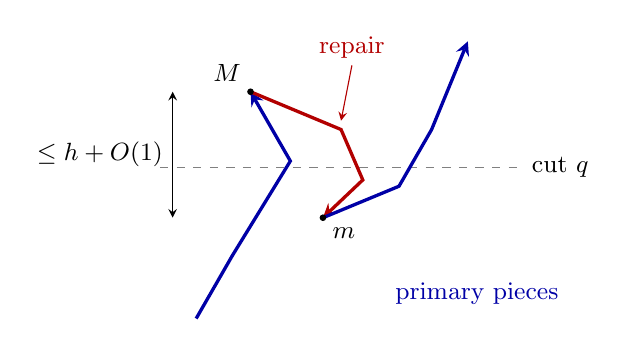
\begin{tikzpicture}[x=2.3cm,y=1.6cm,>=stealth,font=\small]
\draw[dashed,gray](-.2,1.2)--(1.8,1.2)
  node[right,black]{cut $q$};
\draw[very thick,blue!65!black,->]
  (0,0)--(.2,.5)--(.52,1.25)--(.3,1.8);
\draw[very thick,red!70!black,->]
  (.3,1.8)--(.8,1.5)--(.92,1.1)--(.7,.8);
\draw[very thick,blue!65!black,->]
  (.7,.8)--(1.12,1.05)--(1.3,1.5)--(1.5,2.2);
\fill(.3,1.8)circle(1.2pt) node[above left]{$M$};
\fill(.7,.8)circle(1.2pt) node[below right]{$m$};
\draw[<->](-.13,.8)--(-.13,1.8)
  node[midway,left]{$\le h+O(1)$};
\node[blue!65!black]at(1.55,.2){primary pieces};
\node[red!70!black]at(.86,2.15){repair};
\draw[red!70!black,thin,->](.86,2.01)--(.80,1.57);
\end{tikzpicture}
\caption{A repeated crossing of a transverse cut in an upward run.
The segment from the selected maximum $M$ to the following minimum $m$
is read downward; the neighboring pieces are read upward.  The drawing
is schematic and suppresses individual lattice edges.  The drawdown
bound controls the repair's height, while the separated cut levels keep
distinct repairs in ordered disjoint zones.}
\label{R:geo:repair-figure}
\end{figure}

Call the pieces in the original direction primary pieces.  Their spans
are between fixed positive multiples of $h$; repair spans are at most
$Ch$.  After the local port changes, test every turn with sufficiently
large smaller span.  If $P$ is the number of primary pieces, then
\begin{equation}\label{R:geo:primary-count}
                         c d/h\le P\le Cn/h.
\end{equation}
There are at most $P-1$ repairs, and the total modified length is at
most $n+CP$.

Apply Proposition~\ref{R:geo:chain} with $K=h^{3/4}$.  Write a
primary label as $\kappa_i=Kx_i$.  A repair of height scale $a\le Ch$
has $K_{\rm rep}=a^{3/4}$; put
$t=K_{\rm rep}/K$ and $y=\kappa_{\rm rep}/K\le t$.
Fixed comparability constants can be absorbed into all bounds below,
so the normalized labels are at most one.  For a single-crossing cut
without a repair use the formal values $a=K_{\rm rep}=\kappa_{\rm rep}=1$.
This virtual node has unit mass and no avoidance test; its algebraic
node and seam factors are also one, since every actual $\kappa_i\ge1$.

At either kind of cut, smooth the height of the preceding primary
piece.  Its endpoint lies within $O(a)$ of the cut, where the cut level
is specified relative to the run's starting height by the discrete cut
pattern.  We claim that this supplies the factor
\begin{equation}\label{R:geo:repair-smoothing}
                      C\min(1,(t/x_i)^{4/3}).
\end{equation}
Bounded-count nodes use the bounded-factor height estimate in
Proposition~\ref{R:geo:chain}.  At the other nodes, use this constraint
only when $a\kappa_i^{-4/3}<1$, and fix all coordinates outside the
selected reserved groups.  Their height sums
have a joint atom bound equal to the product of their individual bounds
$C\kappa_i^{-4/3}$ from Proposition~\ref{R:geo:chain}.  The allowed
height vectors can be counted in traversal order: once the earlier
selected sums in the run are given, the current endpoint constraint
allows at most $Ca$ values for the next sum.  The run's starting height
cancels from this relative constraint.  Thus the number of allowed
vectors is at most the product of these $Ca$ factors.  Multiplying by
the joint atom bound, and dropping the constraints at the unselected
nodes, proves the product of \eqref{R:geo:repair-smoothing}, since
$a\kappa_i^{-4/3}=(t/x_i)^{4/3}$.  Each primary receives at most one
factor.  This count already includes its possible endpoint heights.
The turn tests use only their separate history and rapid groups in
adjacent-port coordinates; none fixes the displacement of a selected
reserved group.

For completeness, the product calculation is as follows.  A direct
turn between primaries contributes $\max(x_i,x_{i+1})$ after the
primary factors have been collected.  A cut with a repair contributes
\[
 Q=\frac{\max(x_i,y)\max(x_{i+1},y)}{t}
                    \min(1,(t/x_i)^{4/3})
                 \le\max(x_{i+1},y).
\]
If $x_i\le t$, use $y\le t$; if $x_i>t$, the remaining factor is
$(t/x_i)^{1/3}\le1$.  This proves the inequality in both cases,
including the virtual-node convention.  The full product is bounded
by $Kx_1x_P$ times these factors and constant bases.  Every connecting
factor is bounded, and is $O(h^{-s})$ if all its incident labels are
less than $h^{-s}$.  The patterns of runs and cuts, repair scales,
count bins, and local records cost at most
$h^{C\eta(P+1)}$.

Take $s'=\epsilon/2$ and $s=9\epsilon/64$.  For small $\epsilon$
these choices satisfy $9s'/16>s$ and
\[
 \frac{n}{h^{4/3-s'}}=o\bigl(n^{3/4+\epsilon}/h\bigr).
\]
Set $l=h^{4/3-s'}$.  Since the total length is at most $n+CP$,
only $o(P)$ actual nodes have length greater than $l$.  Designate a
superset of these nodes; all possible designations cost at most
$2^{2P}$.  On every other actual node with normalized label at least
$h^{-s}$, the separate short-length group supplies
\[
 C e^{-c k_i q(l)}\le\exp(-h^{c_s}),
\]
for some $c_s>0$: indeed $k_i\ge K h^{-s}$ and
$K h^{-s}q(l)=h^{9s'/16-s+o(1)}$.  Virtual and bounded one-row
nodes have small labels.

If a positive fraction of labels are large, this gives stronger than
exponential decay in $P\log h$.  Otherwise a positive fraction of the
connections have all incident labels small.  Each large or designated
long node can spoil at most two such connections, so those connections
supply $h^{-s}$ each.  Choose $\eta$ sufficiently small after $s$.
After summing all the records and designations, the contribution with
$P$ primary pieces is at most $\exp(-cP\log h)$.  Equation
\eqref{R:geo:primary-count} gives the tall-bridge bound
\begin{equation}\label{R:geo:tall-bridge}
                  \exp(-c d\log h/h).
\end{equation}
All constants are uniform for $d$ in the stated range.

Finally take an unrestricted path of diameter at least $d$.  One of the
finitely many symmetry-related row normals has vertical span at least
$c d$.  In its extremum decomposition from
Proposition~\ref{R:geo:absolute-count}, an initial piece on one of
the two halves reaches the global maximum from the global minimum.
Omit that piece and its neighboring turn tests.  Its individual port
conversion has length at most $n+O(1)$ and height at least $c'd$;
its mass is bounded by \eqref{R:geo:tall-bridge}.  The remaining
pieces, including their choices and records, cost at most
$C_\delta e^{n^\delta}$ for every fixed $\delta>0$.
Choose $\delta$ smaller than the power gain in
$d/h\ge c n^{\epsilon+\gamma}$.  That cost is absorbed by
\eqref{R:geo:tall-bridge}.  This proves
\eqref{R:geo:fast-absolute}.  It also proves the uniform bound
\eqref{R:geo:fast-refined}, since $h\le n^{3/4}$ and the absorbed
exponent is a fixed fraction of $d\log h/h$.
\end{proof}

\section{From renewal pieces to the unrestricted thermal law}\label{R:sec:thermal}
We now prove the full-plane thermal assertion. The proof separates three tasks: identify the half-plane remainder, construct a recoverable family giving the plane denominator, and control paths whose endpoints have small vertical separation. The geometric estimate used in the last task is stated explicitly before the proof.

\subsection{Conventions and prior geometric estimates}
Let $N\ge2$, $z=\rho e^{-1/N}$, and write $w_z(\gamma)=z^{L(\gamma)}$ for vertex length. We count oriented plane walks modulo lattice translations and allow both initial vertex types. Reflection exchanges those types, so the normalized law agrees, after the appropriate reflection and translation, with the thermal law from any fixed vertex. In particular these identifications preserve length, diameter, endpoint distance and absolute endpoint-height difference. If $Z_N$ is this total vertex-weighted mass and $Z_N^{\mathrm{edge}}$ is the edge-weighted sum from one fixed vertex, then
\[
 Z_N=2z Z_N^{\mathrm{edge}}.
\]
This bounded common factor has no effect on the probability laws or moment exponents.

Fix a horizontal row normal. Height is measured in row units; Euclidean vertical distance is $d_0$ times height, where $d_0=\sqrt3/2$. Let $T,L,\Delta$ be the height, vertex length and diameter of an irreducible bridge. The critical probability law is $p$, and
\[
 q_N=1-\E_p e^{-L/N}.
\]
We use the following earlier conclusions of the geometric and irreducible analysis.
\begin{enumerate}
\item Let $B_h$ be the total \emph{critical} mass $\sum\rho^{L(\gamma)}$ of strict bridges from one bottom port at exact height $h$, with terminal port summed. Then
\begin{equation}\label{eq:strip-input}
 B_h\le C(1+h)^{-1/4},\qquad B_0=1,
 \qquad q_N=N^{-9/16+o(1)}.
\end{equation}
The error in the last exponent is an ordinary deterministic asymptotic. It is sufficient here; no bounded-factor length estimate is needed for this thermal transfer.
\item Write $a_m$ for total critical vertex-weighted mass of plane walks of vertex length $m$, in the translation convention just specified. For every $\delta>0$,
\begin{equation}\label{eq:count-input}
 a_m\le C_\delta\exp(m^\delta).
\end{equation}
For every sufficiently small fixed $\eta>0$, there are $c_\eta>0$ and $m_\eta$ such that
\begin{equation}\label{eq:fast-input}
 \sum_{\substack{L(\gamma)=m\\D(\gamma)>m^{3/4+\eta}}}
       \rho^m\le \exp(-m^{c_\eta})\qquad(m\ge m_\eta).
\end{equation}
This is an \emph{absolute critical mass} bound, before division by any probability denominator.
\item We use the two-bridge specialization of the preceding turning-chain estimate. Its exact content for this section is as follows. Consider two bridges with adjacent prescribed bottom ports which stay disjoint for a fixed positive fraction of the smaller height. Restrict each height to an interval $[cH_i,CH_i]$ and each irreducible count to a dyadic interval $[k_i,2k_i)$, for $i=1,2$, with fixed $c,C>0$. The two scales $H_1,H_2$ vary independently; they need not be comparable to each other. All heights and counts are at most a fixed multiple of $N^2$. Put
\[
 K_i=H_i^{3/4},\qquad \kappa_i=\min(k_i,K_i),\qquad
 F=\frac{\kappa_1^2\kappa_2^2}
          {K_1K_2\min(\kappa_1,\kappa_2)}.
\]
For every fixed $\varepsilon>0$, the critical mass in these bins, including the choices of the counts and the bounded endpoint modifications, is at most $C_\varepsilon N^\varepsilon F$. At each bridge with sufficiently large count, the proof reserves a group of irreducibles for a height-concentration test. At bounded counts the displayed height factor below is bounded below by a positive constant, so its inclusion only changes the overall constant. Suppose an interval of at most $C(1+r)$ allowed total heights on bridge $i$ is measurable with respect to the other bridge, the local records, any externally attached remainders fixed up to translation, and the increments of bridge $i$ outside this group. Imposing that interval changes the joint mass bound to
\begin{equation}\label{eq:two-node-input}
 C_\varepsilon N^\varepsilon F
       \min\{1,(1+r)\kappa_i^{-4/3}\}.
\end{equation}
The reserved group is unused by the avoidance and large-height estimates, and its horizontal displacement remains unconditioned and is summed over. The estimate is therefore a joint bound; it does not assert independence after conditioning a bridge on its total height. With a single nonempty bridge the corresponding factor is $\kappa_i^2/K_i$ and the same optional height factor is available. Bounded one-row pieces cost a constant and need no smoothing. There is no additional translation sum at a joining port.
\end{enumerate}
The third input is stronger than a product of unconditioned bridge masses. Its proof uses adjacent-prefix avoidance, height tails and a reserved height-concentration estimate. The bridge-mass and one-piece estimates in \eqref{eq:strip-input} follow from Theorem~\ref{R:renew:finite-input} and Proposition~\ref{R:renew:increments}, respectively. In this section we use it only for two ends created at one minimum. The turning-chain estimate of Proposition~\ref{R:geo:chain}, its two-end specialization in Corollary~\ref{R:geo:two-ends}, and Propositions~\ref{R:geo:absolute-count} and~\ref{R:geo:fast} provide this rule and the absolute count and fast-path bounds. Those arguments concern unnormalized masses and do not use the thermal conclusion. The later uniform-law transfer uses these estimates as well.

\subsection{The terminal remainder and an exact cancellation}
A \emph{half-plane end} begins at a prescribed bottom port, visits vertices strictly above its line and ends at an arbitrary vertex. Its last piece after the highest once-crossed positive row boundary is a half-plane end with no positive renewal boundary. If there is no such boundary, the whole end is the last piece. Let $U_N$ denote the sum of $z$-weights of these no-renewal ends, and let $H_N$ denote the sum over all half-plane ends. Both are finite by \eqref{eq:count-input}; also $U_N\ge z$, from the end consisting of its first vertex.

\begin{lemma}[Half-plane factorization]\label{lem:halfplane}\label{R:renew:halfplane}\label{R:thermal:remainder}
With the conventions above,
\[
 H_N=\frac{U_N}{q_N}.
\]
If a particular ordered tuple of irreducibles has total vertex length $\ell$, the probability under the normalized half-plane $z$-law that it is the initial tuple equals $z^\ell$.
\end{lemma}
\begin{proof}
Factor at all once-crossed positive row boundaries. The factors before the last remainder are strict irreducible bridges, and this factorization is unique. Conversely, adjoining any finite list of irreducibles and a no-renewal end gives a half-plane end. The interiors of successive pieces lie in disjoint height slabs, and the remainder lies above the last joining line. Thus weights multiply and no avoidance correction is needed. A list of $j$ unspecified irreducibles has $z$-mass $(1-q_N)^j$, whence
\[
 H_N=U_N\sum_{j\ge0}(1-q_N)^j=U_N/q_N.
\]
For a prescribed tuple, all possible later pieces together form an arbitrary half-plane end. Its numerator is $z^\ell H_N$, and division by $H_N$ gives the claimed probability.
\end{proof}
This is the same factorization that defines the infinite renewal law, with the honeycomb port convention supplying the adaptation of the finite-prefix argument in~\cite[Propositions~2.2--2.3]{Dyhr2011}. For a fixed tuple, $z^\ell\to\rho^\ell$. Moreover the number of complete irreducibles has the geometric law $q_N(1-q_N)^j$, so it tends to infinity in probability. Hence the fugacity prefix law converges to independent critical irreducibles. This cancellation does not involve a local estimate at any prescribed total length.
Theorem~\ref{R:cal:halfplane-laws} uses this cancellation to prove the half-plane thermal length, spatial and positive-moment laws.

\subsection{A recoverable lower bound for the plane partition function}
\begin{lemma}\label{lem:denominator}\label{R:thermal:denominator}
For all sufficiently large $N$,
\[
 Z_N\ge(q_N^{-1}-1)U_N^2\ge \frac{U_N^2}{2q_N}.
\]
\end{lemma}
\begin{proof}
Take a nonempty bridge from a fixed lower port to an arbitrary upper port. At the lower port attach the reverse of a no-renewal end in the lower exterior half-plane. At the upper port attach a no-renewal end in the upper exterior half-plane. The three pieces have disjoint vertex sets, their weights multiply, and the result is an oriented plane walk.

The construction is injective in the translation convention. In the resulting path, the lowest and highest horizontal row boundaries crossed exactly once are the two attachment lines. There are no single-crossing lines farther outward because both attached ends have no renewals. Recover those two lines from the output, cut at their crossing ports, and translate the lower port to the fixed anchor. This recovers the central bridge and both ends. Internal renewals of the central bridge do not affect this recovery.

The total $z$-mass of all nonempty bridges is
\[
 \sum_{j\ge1}(1-q_N)^j=q_N^{-1}-1.
\]
Multiplying by the two end masses proves the first bound. Since $q_N\to0$, the second follows.
\end{proof}
The factor $U_N$ may be large and is not estimated separately. Its appearance twice in this lower bound is what allows the next numerator estimate to be useful.

\subsection{Small endpoint displacement has small relative mass}
Let $V(\gamma)$ be the absolute difference of the endpoint heights in row units. Since $d_0V\le A\le D$, a lower bound for $V$ gives an endpoint-distance lower bound.

\begin{lemma}[Two-end estimate]\label{lem:twoends}\label{R:thermal:smallheight}
For every $\varepsilon>0$, all sufficiently large $N$ and every $1\le r\le N^2$,
\[
 \sum_{\substack{\gamma\ \mathrm{plane}\\L(\gamma)\le N^2, V(\gamma)\le r}}
       w_z(\gamma)
 \le C_\varepsilon N^\varepsilon(1+r)^{3/4}U_N^2.
\]
\end{lemma}
\begin{proof}
If either endpoint attains the minimum height, use that endpoint as the minimum, reversing orientation if necessary. Otherwise cut at the first internal vertex attaining the minimum. This gives either one half-plane end or two disjoint half-plane ends. The passage between vertex endpoints and ports uses bounded local modifications, with bounded inverse multiplicity and bounded weight factors, uniformly for $\rho/2\le z<\rho$.

Here is the local modification, illustrated in Figure~\ref{fig:minimum}. Write
\[
 u=(1,0),\quad v=(1/2,\sqrt3/2),\qquad
 P_{ij}=iu+jv,\quad R_{ij}=P_{ij}+(u+v)/3.
\]
The neighbors of $P_{ij}$ are $R_{ij},R_{i-1,j},R_{i,j-1}$. An internal lowest vertex must be of type $P$, because a vertex of type $R$ has only one ascending bond. Translate the minimum to $P_{00}$. Keep the branch toward $R_{-1,0}$ and move the start of the branch toward $R_{00}$ to $P_{10}$. If $P_{10}$ is absent, append its free bond to $R_{00}$. If it is present, it cannot be an endpoint, by our initial choice of case. Minimality then forces it to use both ascending bonds, so this branch already reaches it through $R_{00}$; trim that bounded initial segment. Attach the two incoming half-edges from below. The resulting ends start at adjacent ports and remain disjoint. The modification changes only boundedly many vertices, preserves their far endpoints and is undone from a bounded local record.

If a minimum is an endpoint of type $P$, its incoming bottom port gives the one-end representation directly. If it has type $R$ and the path is nontrivial, its first bond is the unique ascending bond; trim that bond and start at its midpoint. No internal vertex can be a lowest $R$. If the other endpoint is also a lowest $R$, trim its last descending bond as well. All remaining vertices then lie strictly above the new starting cut. A singleton walk is handled separately at bounded cost. These operations change the endpoint heights by at most a fixed constant.

\begin{figure}[ht]
\centering
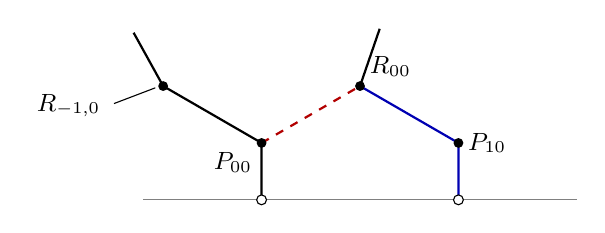
\begin{tikzpicture}[scale=2.5,font=\small]
\draw[gray](-.6,-.289)--(1.6,-.289);
\draw[thick](-.5,.289)--(0,0)--(0,-.289);
\draw[dashed,red!70!black,thick](0,0)--(.5,.289);
\draw[blue!70!black,thick](.5,.289)--(1,0)--(1,-.289);
\draw[thick](-.5,.289)--(-.65,.56);
\draw[thick](.5,.289)--(.6,.58);
\foreach \x/\y in {0/0,.5/.289,1/0,-.5/.289}{\fill(\x,\y)circle(.025);}
\foreach \x in {0,1}{\draw[fill=white](\x,-.289)circle(.025);}
\node[below left]at(0,0){$P_{00}$};
\node[above right]at(.5,.289){$R_{00}$};
\node[right]at(1,0){$P_{10}$};
\node[left]at(-.77,.19){$R_{-1,0}$};
\draw[thin](-.75,.20)--(-.54,.28);
\end{tikzpicture}
\caption{Separating the two branches at an internal minimum. When $P_{10}$ is absent, replace the dashed bond by the blue bond and start the second branch at the right port. When $P_{10}$ is already present, remove the two-bond initial segment through $R_{00}$ instead. The continuations drawn above are schematic.}\label{fig:minimum}
\end{figure}

First suppose there is one end. On the event $V\le r$, its last renewal is at height at most $C(1+r)$. After removing its no-renewal remainder and dropping the restriction on that remainder's final vertex, the mass is at most
\[
 C U_N\sum_{h\le C(1+r)}B_h
       \le C'(1+r)^{3/4}U_N
       \le C''(1+r)^{3/4}U_N^2,
\]
using \eqref{eq:strip-input} and $U_N\ge\rho/2$.

Now suppose there are two ends. Remove their no-renewal remainders and fix those remainders up to translation. Their $z$-weights will be summed at the end. Discard all avoidance constraints involving a remainder and the remaining total-length restriction, but retain the resulting $O(N^2)$ cap on bridge heights and piece counts. Drop the bridge damping factors $e^{-L_i/N}\le1$, so their weights are critical and the third input applies. The remaining two bridges have adjacent starts. If both are nonempty, they remain disjoint throughout the common height range. Put their heights and counts into dyadic bins and use the input's notation. If $a=\min(\kappa_1,\kappa_2)$ and $M=\max(\kappa_1,\kappa_2)$, then $K_i\ge\kappa_i$ gives
\[
 F=\frac{\kappa_1^2\kappa_2^2}{K_1K_2a}\le M.
\]
If $M$ is bounded by the fixed count threshold of Proposition~\ref{R:geo:chain}, the bound without a concentration test is already $O_\varepsilon(N^\varepsilon)$ and suffices. Otherwise choose a bridge $i$ attaining $M$, with a fixed tie rule; its count is large enough to supply the reserved group. In the integration for \eqref{eq:two-node-input}, fix the other bridge, the local records and the increments of bridge $i$ outside its reserved group; the two remainder shapes are already fixed. If $h_j$ is the other bridge's height, the endpoint-height condition restricts the total height of bridge $i$ to
\[
 [h_j+b-r-C_0,\ h_j+b+r+C_0],
\]
where $C_0$ bounds the endpoint-height changes and $b$ is determined by the two remainder endpoint heights and the fixed local records. Subtracting the fixed height of the other increments gives an interval of the same size for the reserved group's height. Its horizontal displacement is still summed over, so this is precisely the permitted concentration test. Thus \eqref{eq:two-node-input} bounds the mass in this pair of bins by
\[
 C_\varepsilon N^\varepsilon M
       \min\{1,(1+r)M^{-4/3}\}
       \le C_\varepsilon N^\varepsilon(1+r)^{3/4}.
\]
The last inequality follows by considering $M\le(1+r)^{3/4}$ and its complement. If only one bridge is nonempty, its factor $\kappa^2/K\le\kappa$ gives the same estimate: bounded $\kappa$ needs no concentration test, and larger $\kappa$ permits the calculation above. If neither is nonempty, the mass is at most one before the remainder weights are restored.

Because $L\le N^2$, there are only $O((\log N)^4)$ pairs of height/count bins. Choose the exponent slack in the geometric input smaller than the desired $\varepsilon$ and absorb this factor. Summing the two fixed remainder weights gives $U_N^2$. Their translations were determined by the bridge tips; no free placement factor is introduced. This proves the bound.
\end{proof}

\subsection{Length, spatial scale and moments}
\begin{samepage}
\begin{theorem}[Unrestricted thermal law]\label{thm:thermal}\label{R:thermal:law}
Choose an ordinary plane honeycomb walk from a fixed vertex with probability proportional to $(\rho e^{-1/N})^n$, where $n$ is its edge length. For every $\xi>0$, its vertex length $L$, endpoint distance $A$ and diameter $D$ satisfy
\[
 \Pp_N\{N^{1-\xi}\le L\le N^{1+\xi},\quad
 N^{3/4-\xi}\le A\le D\le N^{3/4+\xi}\}\longrightarrow1.
\]
For every fixed $p>0$,
\[
 \E_N L^p=N^{p+o(1)},\qquad
 \E_N A^p=N^{3p/4+o(1)},\qquad
 \E_N D^p=N^{3p/4+o(1)}.
\]
\end{theorem}
\end{samepage}
\begin{proof}
We use the equivalent vertex-weighted translation-class law. First record a consequence of \eqref{eq:count-input}. For each $\epsilon>0$, $p\ge0$ and $B>0$,
\begin{equation}\label{eq:damped-tail}
 \sum_{m>N^{1+\epsilon}}m^p a_m e^{-m/N}=O_{\epsilon,p,B}(N^{-B}).
\end{equation}
Indeed choose $0<\delta<\epsilon/(1+\epsilon)$. Uniformly for $m\ge N^{1+\epsilon}$, one has $m^\delta\le m/(2N)$ for all large $N$. The summands are then at most $C_\delta m^p e^{-m/(2N)}$, whose sum has faster than polynomial decay. In particular, paths with $L>N^2$ have negligible absolute mass and negligible mass after multiplication by any fixed length power. Since Lemma~\ref{lem:denominator} gives $Z_N\ge c/q_N$, this remains true after normalization.

Take $r=N^{3/4-\delta}$ with fixed $0<\delta<3/4$. Lemmas~\ref{lem:denominator} and~\ref{lem:twoends} give
\[
 \Pp_N\{V\le r,\ L\le N^2\}
       \le C_\varepsilon N^\varepsilon q_N(1+r)^{3/4}
       =N^{\varepsilon-3\delta/4+o(1)}.
\]
Choose $\varepsilon<3\delta/4$ and add the tail just discarded. It follows that $V\ge N^{3/4-\delta}$ with probability tending to one. After slightly decreasing the exponent tolerance to absorb $d_0$, the same lower bound holds for $A$.

We next obtain the upper spatial estimate from the absolute fast-path bound. Fix $\xi>0$. Choose small positive $\epsilon,\eta$ such that
\[
 (1+\epsilon)(3/4+\eta)<3/4+\xi.
\]
For lengths $m\le N^{1/2}$, the deterministic estimate $D\le Cm$ already gives the desired upper bound for large $N$. For $N^{1/2}<m\le N^{1+\epsilon}$, any violation of $D\le N^{3/4+\xi}$ implies $D>m^{3/4+\eta}$. Summing \eqref{eq:fast-input} over this range gives a faster than polynomially small absolute mass. Lengths above $N^{1+\epsilon}$ are handled by \eqref{eq:damped-tail}. Division by $Z_N$ proves the upper spatial assertion.

The same argument gives the lower length estimate, rather than assuming it from the discount scale. Fix $0<\xi<1$, choose $\eta,\delta>0$ so small that
\[
 (1-\xi)(3/4+\eta)<3/4-\delta,
 \qquad \delta<1/4.
\]
On the typical event $A\ge N^{3/4-\delta}$, a walk of length $m\le N^{1/2}$ is impossible for large $N$. If instead $N^{1/2}<m<N^{1-\xi}$, that endpoint event forces $D>m^{3/4+\eta}$, up to fixed unit factors absorbed by the strict inequality above. The summed exceptional mass is again negligible by \eqref{eq:fast-input}. Hence $L\ge N^{1-\xi}$ with high probability. The upper length bound follows from \eqref{eq:damped-tail}. Larger tolerances follow from smaller ones.

For moments, the lower probability estimates give the respective lower exponents. For the upper length moment, restrict to $L\le N^{1+\epsilon}$ and use \eqref{eq:damped-tail} on its complement:
\[
 \E_N L^p\le N^{p(1+\epsilon)}+o(1).
\]
For the spatial upper moments, repeat the fast-path split with the additional factor $D^p\le C_pL^p$. On the exceptional paths of polynomially large length, the factor is harmless in the sum of \eqref{eq:fast-input}; on the damped long-length tail use \eqref{eq:damped-tail} with this $p$. The remaining paths obey $D\le N^{3/4+\xi}$, apart from the deterministic short-length class. Thus
\[
 \E_N A^p\le\E_N D^p\le N^{p(3/4+\xi)}+o(1).
\]
Let the positive slacks decrease to zero. This completes the proof.
\end{proof}
The proof used the same irreducible law as exact-length conditioning, but a different denominator. It required no estimate of $U_N$, no local renewal mass at length $N$, and no inversion of a density-one statement. The part shared with exact conditioning is the renewal model and its increment estimates; the geometric recovery and two-end smoothing are the additional work needed for the unrestricted thermal law.

\section{Censored arms and absolute spatial estimates}\label{R:cal:geometry-section}
The density-one uniform law will require a bound on the number of ways to
undo an insertion into a walk. Two proposed cuts are valid only if the
exterior arms remain disjoint when one is reflected back toward the other. We estimate this
constraint using independent irreducible histories stopped just before
they reach a prescribed height. Lemma~\ref{R:cal:survival} gives their
survival probability; the kernel calculation in
Section~\ref{R:cal:kernels} transfers it to weighted bridge families.
These are the inputs to the insertion argument in
Section~\ref{R:cal:refolding}.

We use the finite calibrated estimates of Section~\ref{R:cal:section},
with $a=3/4$, $\vartheta=1/4$, $d_*=4/3$, and $\alpha=9/16$.
The same histories also give an independent proof of the absolute
spatial estimates proved in Section~\ref{R:geo:section}. We include that
proof to retain a route from the calibrated inputs alone. Throughout,
$\mu(\omega)=\rho^{|\omega|}$ counts visited centers, ports carry no
weight, and the source is fixed. All masses precede normalization.

\subsection{Finite inputs and the rapid-travel bound}\label{R:cal:fast-section}

The absolute estimate supplied by this route is the following. It will
control upper tails and positive moments after the probability
normalizers have been identified.
\begin{theorem}[Absolute suppression of rapid travel]\label{R:cal:fast}
For every fixed sufficiently small $\xi>0$ there are $c,C>0$ such that the unnormalized critical mass of all plane self-avoiding walks rooted at a fixed center obeys
\begin{equation}
 \sum_{R\le {\rm diam}\,\omega\le 2R,\ |\omega|\le R^{d_*-\xi}}\mu(\omega)
       \ \le\ C\exp(-R^c).                                                   \label{R:cal:fast-mass}
\end{equation}
\end{theorem}
Here $|\omega|$ counts centers; changing to edge count changes the weight by a fixed factor. The proof will follow the survival and kernel estimates below. We first record the finite geometric inputs and their concentration consequences.
We will only need sufficiently large length/distance parameters; all constants below may change by fixed geometric/unit factors.

Keep horizontal integral levels $y$. We use \(B_m\asymp (1+m)^{-\vartheta}\), the exponential diameter cutoff for strict bridges in strips, \(\Pr(D>r)\le C r^{-a}\), \(1-\mathbb E\exp(-tH)\asymp t^a\) and \(1-\mathbb E\exp(-tL)=t^{\alpha+o(1)}\). In particular \(\Pr(H\ge r)\asymp (1+r)^{-a}\). For the lower tail comparison, in \(\mathbb E\min(1,H/T)\gtrsim T^{-a}\) the contribution of \(H<\delta T\) is at most \(C\delta^{1-a}T^{-a}\) by the upper bound integrated in height; take \(\delta\) sufficiently small.

\paragraph{Angular growth and finite chord moments.}
The finite calibrated input also supplies angular growth
\cite[Section~11, Recoverable half-plane growth]{compL}.
For two signed lattice normals making angle $\pi/3$, fix a sufficiently
small relative transverse tolerance $\gamma>0$. There are positive constants
$r_\gamma,K_\gamma,c_\gamma,C_\gamma,C_{1,\gamma}$ such that, for
$r\ge r_\gamma$ and each admissible grid target $S\ge K_\gamma r$,
the construction starts with prefixes at scale $r$ from the fixed source
port on the first wall and continues them to the exact wall of the second
normal at distance $S$, with terminal port free. All centers stay in the first open half-plane and strictly
before the target wall; the mass is at least
$c_\gamma S^{-1/4}(S/r)^{-C_{1,\gamma}}$ and the diameter at most $C_\gamma S$.
During continuation the transverse distance from the second-normal ray
through the selected prefix endpoint is at most $\gamma u$, where $u$
is the second-normal level measured from the original source.
The joining cuts are recovered as the first qualifying singly crossed
walls. The finite flux identity applies on the simple polygonal domains
used below; its coefficient at an exit is the real part of
$\exp(i(3/8)\,\mathrm{turn})$, after a fixed common phase rotation if needed.

Finally, the finite visit identity and planar nesting bound give
\cite[Proposition~11.1]{compL}
\begin{equation}
 \sum_{\substack{\omega\text{ a boundary chord in }Q_R}}
       \rho^{L(\omega)}L(\omega)\le C R^{25/12},
 \label{R:cal:box-moment}
\end{equation}
where $Q_R$ is a convex lattice domain with boundedly many sides and
diameter $O(R)$, and both boundary
ports are summed. Averaging over order-$R$ translates of a fixed boundary
source gives the $CR^{13/12}$ bound used below for paths of diameter at
most $R$. Using a growing diameter cutoff may add logarithmic factors; it
does not produce an unrestricted bounded-factor first bridge moment.

\paragraph{Concentration of independent increments.}
\begin{lemma}[Height and planar displacement atoms]\label{R:cal:atoms}
For $k\ge1$ independent whole irreducibles, with atoms taken on the actual
support lattice,

\[
 \sup_j\Pr(S_H(k)=j)\le C k^{-1/a},\qquad
 \sup_w\Pr(S_{(H,X)}(k)=w)\le C k^{-2/a}. 
\]
\end{lemma}
\begin{proof}
We first obtain a lower tail in the transverse direction. The angular
growth input constructs a positive family of strict bridges of height $h$
whose transverse endpoint displacement has magnitude at least $ch$.
Here are the two stages of that construction.

Start from the bottom port with normals $n=y$ and $u$ making angle
$\pi/3$, at scale $c_*h$. Continue to each exact $u$-level in
$[(2-2\delta_*)h,(2-\delta_*)h]$. Choose the fixed $\delta_*>0$ small,
then $c_*$ and the relative transverse error much smaller than
$\delta_*$. The initial part has diameter $O(c_*h)$, and the
$u$-normal ray gains $y$-height at slope $1/2$. Thus every path remains
in $0<y<h$ and ends at transverse distance at least $ch$, with remaining
height between $\delta_*h/4$ and $2\delta_*h$. Each target has mass
at least $c h^{-\vartheta}$.

Keep only the prefix to the first qualifying single-crossing $u$-cut
in that target bin, testing the confinement and terminal-position
conditions just stated. The total discarded suffix mass is at most
$\sum_{j\le Ch}B_j\le Ch^a$. Summing first over the order-$h$ targets
therefore leaves a family of distinct prefixes of mass at least a
positive constant. From each such prefix, use the angular construction
with normals $u,n$ to reach $y=h$ exactly. This extension lies strictly
beyond the selected $u$-cut, has diameter $O(\delta_*h)$, and has mass
at least $c h^{-\vartheta}$. Its starting scale is a small fixed
fraction of the remaining height, so its diameter constant is independent
of $\delta_*$. For small enough $\delta_*$, the full path remains in
$y>0$ and retains transverse displacement at least $c'h$. The joining
cut is recoverable. Hence
\[
 B_h\{|X_{\rm total}|\ge c'h\}\ge c h^{-\vartheta}.
\]

To pass from this bridge family to one irreducible, use
$|X_{\rm total}|\le\sum_i|X_i|$. On the displayed event,
$\sum_i\min(1,|X_i|/h)$ is bounded below by a positive constant.
The marked-reward identity and the bridge-mass bound give
\[
\begin{aligned}
 c h^{-\vartheta}
 &\le C\sum_{j\le h}\mathbb E_p[\min(1,|X|/h);H=j]
                \sum_{b+d=h-j}B_bB_d\\
 &\le C h^{2a-1}\mathbb E_p\min(1,|X|/h).
\end{aligned}
\]
Thus $\mathbb E_p\min(1,|X|/h)\ge ch^{-a}$.

The off-axis construction and the height estimate must now be combined
uniformly over directions. Put $f_r(z)=\min(1,|z|/r)$. For a unit vector
$(v_1,v_2)$ let $W=v_1H+v_2X$. Reflection in the starting normal preserves
the irreducible law and changes $X$ to $-X$. Since
\[
 f_r(A+B)+f_r(A-B)\ge f_r(A),\qquad
 f_r(A+B)+f_r(A-B)\ge f_r(B),
\]
and at least one $|v_i|$ is at least $1/\sqrt2$, we obtain uniformly in
$(v_1,v_2)$
\[
 \mathbb E f_r(W)\ge c r^{-a},\qquad p(|W|>r)\le C r^{-a}.
\]
For the second bound use $|W|\le C D$ with the fixed coordinate units.
Apply the first bound at scale $\delta r$. Choose fixed $\delta>0$ small
enough that $c\delta^{-a}>2C$. The contribution of $|W|>r$ is then absorbed.
The contribution of $|W|<c'r$ is at most
$C\delta^{-1}(c')^{1-a}r^{-a}$, by the integrated upper tail. Choosing $c'$
sufficiently small after $\delta$ proves
\[
 p(c'r\le |W|\le r)\ge c''r^{-a}
\]
with constants independent of the direction.

Let $\phi(t)=\mathbb E e^{it\cdot(H,X)}$. For small $t\ne0$ use the last
annulus in direction $t/|t|$ with $r=1/|t|$, and symmetrize against an
independent copy of bounded diameter. The absolute phase difference is
between $c'/2$ and $2$ for sufficiently small $|t|$. Consequently
\[
 1-|\phi(t)|^2=\mathbb E[1-\cos(t\cdot((H,X)-(H',X')))]
       \ge c|t|^a.
\]
The random vector $(H,2X)$ lies in $\mathbb Z^2$. Its support differences
have rank two: otherwise a nonzero projection would be constant, contrary
to the directional annuli. A rank-two subgroup of $\mathbb Z^2$ has finite
index. Hence on the Fourier torus $|\phi|=1$ at finitely many points.
At each such point all support phases agree, so the modulus nearby is a
translate of the modulus at zero; on the compact complement it is uniformly
less than one. Fourier inversion thus bounds every atom by a constant times
\[
 \int_{\mathbb R^2}e^{-ck|t|^a}\,dt=C'k^{-2/a}.
\]
The one-dimensional argument for $H$, allowing its own finite set of peaks,
gives $Ck^{-1/a}$. No conditioning on the length of any irreducible has
been used.

\end{proof}

\begin{lemma}[Short bridges at a specified height]\label{R:cal:short}
For fixed small \(\delta>0\), some \(v_0,\sigma_0>0\) give uniformly for \(S^{1-v_0}/2\le m\le C S\),
\begin{equation}
 B_m\big(|\omega|\le S^{d_*-\delta}\big)\le C m^{-\vartheta} S^{-\sigma_0}.          \label{R:cal:short-height}
\end{equation}
\end{lemma}
\begin{proof}
Here and below $B_m(\cdot)$ denotes restricted bridge mass.
First sum over counts $k>m^{a-\theta}$. Exponential damping in length
bounds the short-length event by
\[
 p\{S_L(k)\le S^{d_*-\delta}\}
 \le \exp\{1-kq_L(S^{-d_*+\delta})\}.
\]
For $m\ge S^{1-v_0}/2$, choose $\theta,v_0>0$ sufficiently small
after $\delta$. The exponent is then at most $-S^c$ for some $c>0$.
There are at most $m$ counts.

For $k\le m^{a-\theta}$, put $t_0=m^{1-z}$ with $0<z\ll\theta$.
If all height jumps are at most $t_0$, positive exponential weighting
bounds the probability of attaining $m$ by
\[
 e^{-m/t_0}(1+C t_0^{-a})^k
 \le \exp\{-m^z+C m^{-\theta+az}\},
\]
which is smaller than every inverse power of $m$. Otherwise select a
jump exceeding $t_0$ and apply the height atom bound to the other
increments. Its cost is at most
$Ck m^{-a(1-z)}k^{-1/a}$; for $k=1$, the height tail gives the same
bound directly. Summing these terms yields
\[
 C m^{-a(1-z)}\sum_{k\le m^{a-\theta}}k^{1-1/a}
 \le C m^{a-1-\theta(2-1/a)+az}.
\]
Since $2-1/a>0$, choose $z$ so that the exponent has a fixed saving
below $a-1=-\vartheta$. The comparison $m\ge S^{1-v_0}/2$ turns
that saving into $S^{-\sigma_0}$, as required.

\end{proof}

\subsection{Two censored arms}\label{R:cal:censored}

\begin{lemma}[Censored two-arm survival]\label{R:cal:survival}
Start two independent sequences of irreducibles from the same bottom port \(p\) with first center \(v\). On each keep its history of completed pieces up to heights \textbf{strictly less} than \(g\), not including the first jump reaching or passing \(g\). Fix roles left, right. Impose the following constraints whenever \(0<d_1<d_2<g\) are cut heights in the left, right history respectively. The prefixes to them, apart from the shared start through \(v\), must go disjointly (leaving \(v\) on the two respective sides). At level \(d_1\) all crossings of the right prefix must be to the right of \(x_1\), the terminal horizontal coordinate of the left prefix. Write \(f(g)\) for the probability of these constraints. Then for each \(\eta>0\)
\begin{equation}
 f(g)\le C_\eta (1+g)^{-a+\eta}.                                             \label{R:cal:survival-bound}
\end{equation}

\end{lemma}

\begin{figure}[ht]
\centering
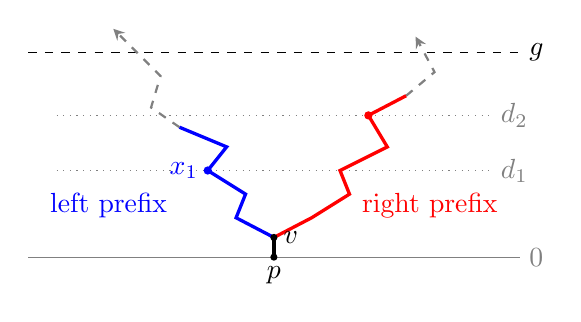
\begin{tikzpicture}[x=1.2cm,y=1cm,>=stealth]
 \draw[gray] (-2.6,0)--(2.6,0) node[right] {$0$};
 \draw[dashed] (-2.6,2.6)--(2.6,2.6) node[right] {$g$};
 \draw[gray,dotted] (-2.3,1.1)--(2.3,1.1) node[right] {$d_1$};
 \draw[gray,dotted] (-2.3,1.8)--(2.3,1.8) node[right] {$d_2$};
 \draw[very thick] (0,0)--(0,.25);
 \draw[very thick,blue] (0,.25)--(-.4,.5)--(-.3,.8)--(-.7,1.1)
    --(-.5,1.4)--(-1,1.65);
 \draw[very thick,red] (0,.25)--(.4,.5)--(.8,.8)--(.7,1.1)
    --(1.2,1.4)--(1,1.8)--(1.4,2.05);
 \draw[thick,gray,dashed,->] (-1,1.65)--(-1.3,1.9)--(-1.2,2.3)--(-1.7,2.9);
 \draw[thick,gray,dashed,->] (1.4,2.05)--(1.7,2.35)--(1.5,2.8);
 \fill (0,0) circle(1.3pt) node[below] {$p$};
 \fill (0,.25) circle(1.3pt) node[right] {$v$};
 \fill[blue] (-.7,1.1) circle(1.5pt) node[left] {$x_1$};
 \fill[red] (1,1.8) circle(1.5pt);
 \node[blue] at (-1.75,.65) {left prefix};
 \node[red] at (1.65,.65) {right prefix};
\end{tikzpicture}
\caption{The two histories share their first center $v$. Only complete
irreducibles ending strictly below $g$ are retained; the dashed continuations
are the omitted crossing pieces. At a tested left renewal level $d_1$, all
crossings of the right prefix ending at a higher tested level $d_2$ must lie
right of $x_1$. The paths are schematic, rather than lattice embeddings.}
\label{R:cal:censor-figure}
\end{figure}

\begin{proof}
There are two estimates to combine. A test with substantial transverse
clearance is rare by a positive flux comparison. After any candidate for
the last such test, each later test costs a power through either a large
height increment or a small transverse interval. Those later costs use
fresh coordinate blocks.

\paragraph{Test scales.}
Put $s=g$ large. Fix constants $0<\ell\ll\lambda\ll b\ll\kappa_0\ll1$, in particular
$b>2\lambda$, $\lambda\ge\ell$, and
$\kappa_0>b+2\lambda+a\ell$. These inequalities ensure that the normal
heights are separated, all tests lie below $g$, and each proximity test has
the saving used below. Use \(r_j=s^{\kappa_0+j\ell}\), \(0\le j\le J=\lfloor(1-2\kappa_0)/\ell\rfloor\). Test at piece indices sampled independently, uniform over integers \([A_{i,j}^a,2A_{i,j}^a]\) on the two uncensored sequences, where \(A_{1,j}=r_j,\ A_{2,j}=r_j s^b\) respectively. These index ranges are increasing and separated for large \(s\). Write \(d_i\) at a test for its cumulative heights; call them normal if each is in \([A_{i,j}s^{-\lambda}, A_{i,j}s^\lambda]\), implying \(1\ll d_1\ll d_2<g\). The chance of falling below such a range at any test is superpolynomially small by height damping. At normal heights we may also require both prefix diameters at most \(d_i\log^2 s\), except at superpolynomially small cost (sum the exponential strip diameter tail at the possible exact heights; a prefix at the given index has precisely its irreducible-product mass).

\paragraph{Separated tests and positive flux.}
Call a test separated if these normality, diameter and two-prefix constraints hold and the horizontal clearance between \(x_1\) and the leftmost right-prefix crossing at \(d_1\) is at least \(\chi d_2\), where \(\chi=s^{-\kappa_0}\). Unconditionally, its probability is at most
\begin{equation}
 C r_j^{-a}s^{\kappa_0+a\lambda}(1+\log s)^C.                               \label{R:cal:separated-test}
\end{equation}
Here are the gluing details. Sort \(d_2\) into dyadic bins \(d_2\asymp H\). Translate both paths together so the line at \(d_1\) becomes \(y=0\), and a lattice corner chosen strictly in the clearance gap becomes the origin; this allows at least \(c\chi H\) placements per input. The top line is now \(y=\Delta=d_2-d_1\asymp H\). Work inside a parallelogram of triangles with this top, bottom at \(-C H\) (rounded outward), and slant side walls allowing all paths by width \(O(H\log^2 s)\) with ample margin. Slit it along \(y=0\) from its left wall to the origin (split the corresponding ports into two boundary copies). Joining the prefixes at \(v\), removing the common initial half-edge, gives a simple chordal arc from a top wall port to the lower lip of the slit. It has no other boundary contact. To mark the choice of \(v\) among deepest vertices, use the hexagonal face centered at the bottom-left corner of \(v\)'s triangle. Its only vertices at height \(\ge y(v)\) are \(v\), a second minimum-height candidate at its left, and their common higher neighbor. The edge from \(v\) to that neighbor is used; if the second candidate is visited it must also use its edge to the same neighbor (minimum height and not an endpoint). Thus exactly a contiguous one- or two-edge arc of the face is present. Replace by the complementary face arc, giving a unique deepest vertex and hence identifying the face. This lies far from the domain boundaries. The change and joining have bounded weight costs. Inverse multiplicity is bounded since we can undo at that face and recover both original prefixes by translating \(v\) back (and the slit placement is determined).

Figure~\ref{R:cal:slit-figure} shows the resulting domain and the clipping operation used in the flux comparison.

\begin{figure}[ht]
\centering
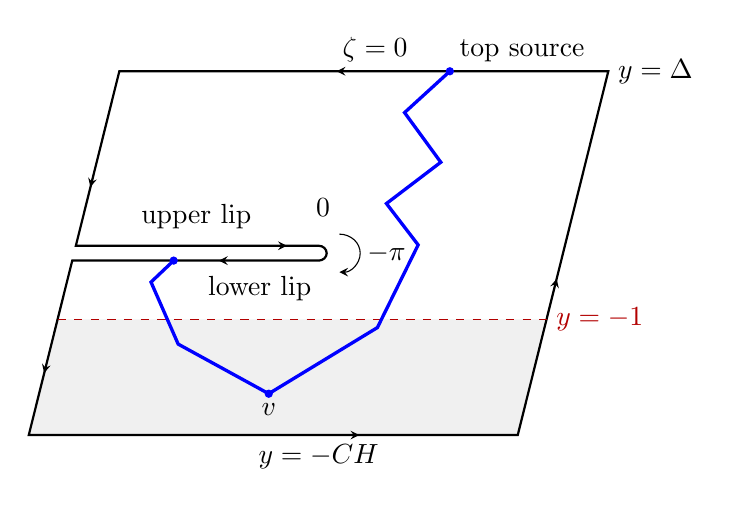
\begin{tikzpicture}[x=1.15cm,y=1.05cm,>=stealth]
 \fill[gray!12] (-2.882,-.8)--(2.518,-.8)--(2.2,-2.2)--(-3.2,-2.2)--cycle;
 \draw[thick] (1.45,2.2)--(-2.2,2.2)--(-2.68,.09)--(0,.09)
   arc[start angle=90,end angle=-90,radius=.09]
   --(-2.72,-.09)--(-3.2,-2.2)--(2.2,-2.2)--(3.2,2.2)--cycle;
 \draw[->] (1.05,2.2)--(.2,2.2) node[midway,above] {$\zeta=0$};
 \draw[->] (-2.35,1.54)--(-2.52,.8);
 \draw[->] (-1.1,.09)--(-.35,.09);
 \draw[->] (-.35,-.09)--(-1.1,-.09);
 \draw[->] (-2.84,-.61)--(-3.03,-1.45);
 \draw[->] (-.45,-2.2)--(.45,-2.2);
 \draw[->] (2.43,-1.18)--(2.63,-.31);
 \draw[->] (.23,.23) arc[start angle=90,end angle=-90,radius=.23];
 \node at (.75,0) {$-\pi$};
 \node[above] at (-1.35,.18) {upper lip};
 \node[below] at (-.65,-.16) {lower lip};
 \node[above] at (.05,.32) {$0$};
 \draw[red!70!black,dashed] (-2.882,-.8)--(2.518,-.8)
   node[right] {$y=-1$};
 \draw[very thick,blue] (1.45,2.2)--(.95,1.7)--(1.35,1.1)
   --(.75,.6)--(1.1,.1)--(.65,-.9)--(-.55,-1.7)
   --(-1.55,-1.1)--(-1.85,-.35)--(-1.6,-.09);
 \fill[blue] (1.45,2.2) circle(1.5pt) node[above right,black] {top source};
 \fill[blue] (-1.6,-.09) circle(1.5pt);
 \fill[blue] (-.55,-1.7) circle(1.5pt) node[below,black] {$v$};
 \node[right] at (3.2,2.2) {$y=\Delta$};
 \node[below] at (0,-2.2) {$y=-CH$};
\end{tikzpicture}
\caption{The slit domain for a separated test, before the bounded modification at the deepest face. The joined prefixes form the blue arc from the top source to the lower lip; their original common minimum $v$ lies below the clipping line. Boundary arrows specify the counterclockwise traversal, including its clockwise half-turn at the slit tip. The slit is drawn with positive thickness, and the vertical spacing is not to scale. The lifted-angle calculation in the proof supplies positivity of the flux coefficients.}
\label{R:cal:slit-figure}
\end{figure}

From each fixed top source, the mass in this slit domain of arcs as produced is \(\le C H^{-\vartheta}\). Indeed they are lost on clipping to \(y\ge-1\). The boundary extension identity from that source has uniformly positive real coefficients before and after clipping, unchanged to retained exit ports. Traversing counterclockwise starting west on the top, the lifted tangent travels down the left side, east along the upper lip, turns clockwise by \(\pi\) to west along the lower lip, continues down the left wall then around via the bottom, right wall and top. All lifted boundary tangent angles $\zeta$ relative to the start lie in
$[0,2\pi]$. Closing an arc along that boundary gives its turn as
$\zeta-\pi$: the two endpoint half-edge corners each add $\pi/2$.
Consequently its real flux coefficient is
$\cos((3/8)(\zeta-\pi))\ge\cos(3\pi/8)>0$, which supplies the required
uniform positivity.

More explicitly, the finite extension identity sums with the slit adjacencies forbidden (detour reversals valid since the source on the top is approached from outside any such cycle); slit ends of half-edges are boundary terms. For the simple arc turn calculation one can thicken the slit by an arbitrarily narrow indentation, trimming terminal half-edges at lip ports slightly if needed: other arc edges stay off the slit, including its corners, and the lifts at source and exit are as stated. Thus this also follows by closing in a simple boundary polygon.

Positive lost mass is bounded by the new exits' mass, and those exits are a subset of strict downward bridges of height \(\Delta+1\). This proves the claim. Summing over \(O(H\log^2 s)\) top ports and \(O(H)\) choices of \(\Delta\), and dividing by placements, gives \(O(\chi^{-1}H^a\log^2 s)\) cumulative input mass. The probability of each prefix pair at the test has, besides its bridge mass, index factors at most \(C r_j^{-a}(r_j s^b)^{-a}\) by uniform sampling (piece counts uniquely specified). Since \(H\le C r_j s^{b+\lambda}\), this gives \eqref{R:cal:separated-test}.

\paragraph{Fresh blocks after a candidate last separated test.}
Choose an index $p_0$ and require only that its test is separated.
Condition on all sampled indices and on both sequences through the test
at $p_0$. We do not condition on its being the last separated test.
For $p_0=-1$, expose no increments. We bound the event that the
survival constraints hold and that no later test is separated.

At every $j>p_0$, either a cumulative height exceeds
$A_{i,j}s^\lambda$, or the test has normal heights and its left endpoint
lies within $\chi d_2$ to the left of the minimum right-prefix crossing
at level $d_1$. The small-height and excessive-diameter cases were
already discarded. In the large-height case, some fresh index block
$q$, with $p_0<q\le j$, has gained at least $c_J A_{i,j}s^\lambda$.
The exposed height at $p_0$ is negligible compared with this threshold.
Assign such a side and block to the test; there are only a bounded
number of assignments, since $J$ is fixed. If several tests select one
block, keep its requirement for the largest $j$.

A block on side $i$ has at most $2A_{i,q}^a$ increments. The height-sum
tail therefore bounds its assigned event by
\[
 C_J s^{-a((j-q)\ell+\lambda)}
 \le C_J s^{-a\ell(j-q+1)}.
\]
Thus this one block pays for every test in the index interval $[q,j]$.
For each index outside the union of these intervals we use the
transverse proximity condition instead.

To estimate a proximity test, fix the entire relevant right sequence
and all earlier left blocks. The last left block contains order
$r_j^a$ fresh increments, so its joint endpoint atom is at most
$Cr_j^{-2}$ by Lemma~\ref{R:cal:atoms}. There are at most
$Cr_js^\lambda$ allowed left heights. At each one, the right sequence
specifies a transverse interval of length at most
$s^{-\kappa_0}r_js^{b+\lambda}$, which is at least one and hence also
bounds the number of lattice sites up to a constant. This gives the
uniform conditional bound
\[
 C r_j^{-2}(r_js^\lambda)
                (s^{-\kappa_0}r_js^{b+\lambda})
 = C s^{b+2\lambda-\kappa_0}
 \le C s^{-a\ell}.
\]
The left blocks used here are distinct and have not been assigned
large-height events. Their bounds multiply after the right sequence
has been fixed. The required large-height estimates for the right
blocks then multiply by their independence. Integrating left blocks
in reverse order gives the same conclusion for assigned left blocks
and proximity tests together. If $\mathcal C$ is the union of assigned
index intervals, the resulting cost is at most
\[
 C_J s^{-a\ell|\mathcal C|}
       s^{-a\ell(J-p_0-|\mathcal C|)}
 = C_J s^{-a\ell(J-p_0)}.
\]
Overlaps between assigned intervals only improve this upper bound.

\paragraph{Combining the two estimates.}
Every surviving pair has either a last separated test or none. For a
candidate $p_0\ge0$, multiply its unconditional bound
\eqref{R:cal:separated-test} by the uniform fresh-block bound just
proved. For no separated test use that bound with $p_0=-1$. Summing
over the finitely many candidates gives
\[
\begin{aligned}
 f(s)
 &\le C_J s^{-a\ell(J+1)}
   +C_J\sum_{p_0=0}^J
       r_{p_0}^{-a}s^{\kappa_0+a\lambda}(1+\log s)^C
       s^{-a\ell(J-p_0)}
   +s^{-M}\\
 &\le s^{-a+O(\kappa_0)+o(1)}.
\end{aligned}
\]
Here $M$ can be arbitrarily large, accounting for the discarded cases.
Choose $\kappa_0$ and then the smaller parameters so that the exponent
loss is less than the prescribed $\eta$. Enlarging the constant covers
bounded $s$ and proves \eqref{R:cal:survival-bound}.

\end{proof}

\subsection{Summing the cores between censored ends}\label{R:cal:kernels}

The preceding lemma is a probability estimate for two independent
histories. A bridge of prescribed height does not have independent ends.
We now express its positive weight relative to the independent history
laws, keeping a kernel for the pieces between them. Uniform bounds on
that kernel will justify using the survival estimate in weighted counts.

\paragraph{Endpoint conventions and the retained turn constraints.}
Decompose a walk into weak bridges with center endpoints, allowing ties
in height and cuts at singly crossed wall ports. Extend each piece to
exterior wall ports with an outward half-edge and, if necessary, one
additional center at each end. At a turn the common vertex is a height
extremum, with both used edges pointing toward the interior. The same
outward port can therefore be used for both virtual extensions. At a
lower turn they both begin $p\to v$ and then leave on opposite slants,
as in Lemma~\ref{R:cal:survival}. Their virtual starts are allowed to
coincide. Multiplying the strict-piece weights costs at most $C^k$ for
$O(k)$ pieces, accounting for duplicated or added centers. Recording the
local extensions and trimming choices also costs $C^k$ and recovers
the original anchored walk. Each span changes by a bounded amount.

At a turn use either the vacuous threshold $g=1$ or a threshold well
below both adjacent heights. Then the tested prefixes and their
continuations stay before the far endpoint modifications. They are
disjoint after $v$ because they come from disjoint arms of the original
walk. For the order condition, continue the left prefix to its first
hit of the higher tested level $d_2$. This is a strip crosscut meeting
its renewal level $d_1$ only once. The right arm leaves $v$ to its
right and cannot cross it, so all right-prefix crossings at $d_1$ lie
to the right of the left endpoint. Thus the survival constraints hold.
Reflection or reversal handles other turns, with at most a constant
choice of roles per turn.

\paragraph{The density relative to independent histories.}
Write $T(t)=p(H\ge t)$ and $p_j=p(H=j)$. If $\xi$ is a list of
complete irreducibles of total height $b<g$, its probability as the
history censored before $g$ is
\[
 \mathsf P_g(\xi)=\mu(\xi)T(g-b).
\]
The extra factor records that the next, omitted jump reaches or passes
$g$. In particular $T(g-b)\ge c g^{-a}$.

Consider a strict bridge of height $h$. Let $\xi_L,\xi_R$ be the
histories read inward from its two ends, with heights $b<g_L$ and
$d<g_R$. Put $T_L=T(g_L-b)$ and $T_R=T(g_R-d)$. We choose the
thresholds so that $h-b-d\asymp h$. Relative to
$\mathsf P_{g_L}\otimes\mathsf P_{g_R}$, the remaining mass is bounded
by the sum of two kernels:
\[
\begin{aligned}
 K_h^{\rm same}(\xi_L,\xi_R)
   &=\frac{p_{h-b-d}}{T_LT_R},\\
 K_h^{\rm distinct}(\xi_L,\xi_R)
   &=\mathbb E\!\left[
        B_{h-b-d-Y_L-Y_R}\,;\ h-b-d-Y_L-Y_R\ge0
        \ \middle|\ Y_L\ge g_L-b,\ Y_R\ge g_R-d
      \right].
\end{aligned}
\]
Here $Y_L,Y_R$ are independent copies of $H$. In the first case the
same irreducible crosses both thresholds; in the second, the two
crossing irreducibles are distinct and the bridge between them has
height $h-b-d-Y_L-Y_R$. A total-length upper bound on the original
piece may also be imposed on this middle bridge, replacing $B_m$ by
its restricted mass. All other restrictions can be dropped for an
upper bound.

These formulas follow by irreducible factorization. They keep the
survival-tail denominators supplied by the censored laws; those factors
cannot be omitted when passing from probabilities to weighted bridges.
No final transverse coordinate is prescribed. The terminal port is
fixed by translating the reversed suffix to the end of the middle
piece, so there is no additional placement factor.

\paragraph{Integration rule for a chain.}
For a chain of pieces take the product reference measure $\mathsf P$
of all its left and right censored-history laws. Retain only the chosen
turn indicators $\mathbf1_{E_v}$. Each indicator involves a disjoint
pair of end histories, aligned at their common turn. Choose their
thresholds from coarse data, independently of the fine height variables
still to be summed. With $K_i=K_i^{\rm same}+K_i^{\rm distinct}$, the
weighted chain sum is bounded, up to its recorded $C^k$ endpoint cost,
by
\[
 \int \left[\sum_{\boldsymbol h\in\mathcal A}
                  \prod_i K_i(h_i;\xi_{i,L},\xi_{i,R})\right]
          \prod_v\mathbf1_{E_v}(\boldsymbol\xi)
          \,d\mathsf P(\boldsymbol\xi),
\]
where $\mathcal A$ denotes the retained height constraints. If the
bracket is at most $C_*$ uniformly in the histories, this is at most
\[
 C_*\prod_v f(g_v).
\]
Thus the order is: fix the histories, sum the kernels over fine heights,
and only then integrate the independent turn indicators. The physical
weighted bridge family itself is not asserted to have independent ends.
Both the volume bound below and the insertion-label argument use this
rule; the latter needs only its one-ended version.

\begin{proposition}[Critical mass in a bounded region]\label{R:cal:volume}
Let \(V_R\) denote the mass of all center walks from a fixed center with diameter at most \(R\). We have for every \(\nu>0\)
\begin{equation}
 V_R\le \exp(C_\nu(1+R)^\nu).                                                \label{R:cal:volume-bound}
\end{equation}
\end{proposition}
\begin{proof}
Split at a lowest point (polynomial placement cost), then decompose each direction into weak bridges by repeatedly cutting at the last occurrence of the opposite extremum of the remaining path. On each chain spans are decreasing, strictly except possibly the second equal to the first. Group consecutive spans in dyads \([s,2s)\). In such a group of size \(k\), \(1\le k\le C s\), only impose shared-turn constraints \emph{within} the group. Strict heights \(h\asymp s\) there differ only boundedly from the weak spans. Assume \(s\) large (bounded small dyads cost a constant by the ordinary bridge bounds); take common threshold \(g=\max(1,\lfloor c_*s/k\rfloor)\asymp s/k\) for small fixed \(c_*\).

Call a piece exceptional in this sum if the threshold jumps coincide or are distinct with middle height \(m<g\). Its kernel summed over the height dyad costs at most \(C s^a k^{-2a}\). Indeed the coincident case uses the tail at \(h-b-d\gtrsim s\) summed at distinct heights, and the two \(T\) factors. In the other case one jump is of order \(s\), giving conditional probability \(\le C(g/s)^a\); sum also \(\sum_{m<g}B_m\le Cg^a\). For ordinary pieces (\(m\ge g\)) the kernel per fixed \(h\) costs \(\le C s^{-\vartheta}\): for \(m\asymp s\) this is direct, for \(m\) smaller use \(B_m\le C g^{-\vartheta}\) and the large jump factor \((g/s)^a\) again. For \(t=k-r\) ordinary pieces with \(r\) exceptional, we retain height ordering constraints among just the ordinary ones, giving at most \(C^k s^t/t!\) ordinary lists (original spans are ordered on the discrete grid, \(t\le Cs\), and bounded perturbations cost boundedly per piece). Exceptional heights sum without ordering. Multiply now by \(k-1\) pair factors \eqref{R:cal:survival-bound}. Uniformly from the fixed group start the total, absorbing subset choices, is at most
\[
 C_\eta^k s^{ak}\, k^{-2ar}(t!)^{-1}\,(s/k)^{(-a+\eta)(k-1)}
       \le s^a\big(C'_\eta s^\eta/k^\vartheta\big)^k ,
\]
with the last bound also covering the sum over types (\(1/t!\le \exp(k)/k^t,\ 2a>1\)). Summing \(k\) and multiplying over \(O(1+\log R)\) dyads on each chain proves \eqref{R:cal:volume-bound}, taking \(\eta\) sufficiently small depending on \(\nu\) (terms with \(k\) above a constant times \(s^{2\eta/\vartheta}\) already decay). We overcount freely between groups/chains.

\end{proof}

\subsection{Subdivision for fast crossings}\label{R:cal:subdivision}

\begin{proof}[Proof of Theorem~\ref{R:cal:fast}]
An input of \eqref{R:cal:fast-mass} contains a weak bridge between a minimum and maximum in some signed normal direction of span \(H\asymp R\), since the three lattice directions control diameter; take the sign so it is oriented from low to high. We call this coordinate \(y\) again. The exterior pieces cost at most \(V_{2R}^2\) up to constants; it suffices to estimate such weak bridges from their fixed first vertex. Pay \(O(R)\) for specifying the last height and normalize the first height by translation.

Take \(\delta=\xi/2\), small \(0<\sigma\ll\xi\), integer \(S\asymp R^{1-\sigma}\), so \(R^{d_*-\xi}=o(S^{d_*-\delta})\). First divide the bridge into swings with drawdown/up threshold \(s_0=S/10\). Track running maxima from the beginning; on first detecting a fall by at least \(s_0\) from one, mark the last corresponding peak before detection and switch to tracking running minima starting at detection, with next switch symmetrically after a rise, marking the trough, and so on. Use the marked extrema (not the detection points) and the two endpoints to cut. Every resulting swing is a weak bridge of span \(\ge s_0\), with adverse increments between any earlier and later point of that swing strictly less than \(s_0\). Indeed, e.g. on an upswing the initial trough-to-rise-detection part lies above the trough, and strictly within \(s_0\) above it before detection. From detection to the peak the running maximum rule gives the bounds; all heights stay above the trough and at most the peak on both parts. The reversed argument works going down, and the global endpoint extrema handle first/last swings (after detecting a fall there must still be a rise by threshold before or at the terminal maximum). Without any switch the span itself is \(H\).

Inside each swing use all absolute grid levels spaced by \(S\) (multiples of \(S\) in wall coordinates) with interior margin \(\ge 2s_0\) from both extrema. Here is the subdivision in upward orientation, symmetrically otherwise. For each such level \(l\), if there is just one crossing, cut there at the port. Otherwise take a highest vertex \(A_l\) before the last upward crossing of \(l\), and a lowest \(B_l\) after \(A_l\) in this swing. Then \(y(A_l)>l>y(B_l)\), both are between the first and last crossings (a return occurs after \(A_l\), all vertices after last crossing are above). The path between them is a descending weak bridge of span \(<s_0\); mark it as an inserted piece. These crossing zones for successive levels occur in order since a backtrack of size \(S\) is impossible. All intermediate pieces are upward weak bridges: e.g. from \(B_l\) to \(A_{l+S}\) all vertices respect those extremal bounds, with the analogous inequalities at single crossings and swing endpoints. These \textbf{main} pieces have spans between \(c S\) and \(C S\), by the margins, offsets \(<s_0\) and the minimum full swing span if no cut. Thus throughout the original bridge there are \(k\ge c H/S\) main pieces and at most \(k\) inserts.

Use strict virtual pieces with the bounded endpoint extensions described above. Specify their types/order, signs, and the following boundary data, at cost \(R^{O(1)}(C(1+\log R))^{C k}\) before any fine coordinates at turns:
\begin{itemize}
\item At a turn between swings, label the coarse height interval (grid of size \(S\)) and assign boundary scale \(D_j=S\).
\item At the two turns for an insert, label the grid level and a common dyad \(D_j\asymp 1+|y(A_l)-y(B_l)|\) (same at both). Each height has offset \(O(D_j)\) from that level.
\item At the single-cut ports label the grid level; take \(D_j=1\) there and at the prescribed endpoint heights.
\end{itemize}

Coarse coordinates cost boundedly many choices per piece from those before, since increments are \(O(S)\). We can include any finite endpoint/port adjustment types as labels. Thus each virtual boundary height \(w_j\) still to sum ranges over \(O(D_j)\) possibilities (already fixed at external endpoints and single cuts), and for fixed next \(w_{j+1}\) has bounded multiplicity per intervening strict-piece height \(h\), their signed difference. We restrict \(h\asymp P\), where \(P=S\) on main pieces, \(P=D_j=D_{j+1}\) on inserts; other fine height ordering restrictions will not be needed. Every strict piece length is \(\le S^{d_*-\delta}\) by the global input bound, including its bounded adjustments.

Use \eqref{R:cal:short-height}, and fix \(0<u\ll v\ll \min(v_0,\sigma_0)\). Call a boundary active if \(D_j\ge S^{1-v}\). At scale \(D'=D_j\) take the threshold
\[
 g(D')=\max(1,\lfloor c_*D'S^{-u\,{\bf1}_{\rm active}}\rfloor)
\]
for small fixed \(c_*\). Since each endpoint scale is \(O(P)\) this ensures \(h-b-d\asymp P\) at the censored kernel, and pair tests at turns are either vacuous or well below the adjacent far adjustments. Write \(F(D')=C_\eta g(D')^{-a+\eta}\) as a pair bound, or \(1\) at unpaired boundaries with \(D'=1\).

The subdivision has reduced rapid travel to many main pieces of scale $S$.
It remains to extract a power saving from each such piece without spending
the same independent end history twice.

We sum each kernel over its \emph{left} boundary height at fixed right height and histories from both ends (left/right here meaning first/last in traversal). Include in its numerical budget also the factor \(F(D_L)\) at the first boundary of that piece. We claim a bound \(S^{-c_1}\) for this product on main pieces and active-scale inserts, for some \(c_1>0\) uniformly at all sufficiently small \(\eta\); on inactive-scale inserts at most \(C_\eta S^{2\eta}\) suffices.

Indeed in the coincident-jump case the summed kernel is at most \(C g_L^a g_R^a P^{-a}\), using bounded multiplicity per height. With \(F(D_L)\) this leaves \(O_\eta(S^\eta (g_R/P)^a)\), giving the claim (on main pieces \(g_R/P\le C\max(S^{-v},S^{-u})\), and on active inserts \(\le CS^{-u}\)). In the distinct case sort \(1+m\) in dyads of scale \(M\). For fixed crossing increments each \(m\) can occur boundedly often as the left height varies, with \(O(D_L)\) possible heights total. Thus by \(B_m\le C M^{-\vartheta}\) we have kernel bound
\[
 C\min(D_L M^{-\vartheta},M^a)
   = C D_L^a\min((D_L/M)^\vartheta,(M/D_L)^a).
\]
Here \(D_L^a F(D_L)\le C_\eta S^\eta\) times \(S^{a u}\) if active. When \(M\ge S^{1-v_0}\) \eqref{R:cal:short-height} allows multiplying by \(S^{-\sigma_0}\), enough. For smaller \(M\) on a main piece or active insert, there must be a giant crossing jump \(y_i\ge cP\) on some side \(G\). Accordingly we can multiply the bound, after splitting into the two possible sides, by \(C (g_G/P)^a\) by its conditional tail. On a main piece this saves \(S^{-av}\) if \(G\) inactive, otherwise \(S^{-au}\); on an active insert (both sides active) also \(S^{-au}\). In the latter savings cases, if left itself is active and pays \(S^{au}\), the factor \((M/D_L)^a\le S^{-a(v_0-v)}\) supplies the gain. Inactive inserts just use the unconstrained dyad estimate with both boundary scales inactive. For clarity, all these cases have a common strictly positive saving before
the small $\eta$ loss:
\[
 \Lambda=\min\{au,\ a(v-u),\ a(v_0-v),\ \sigma_0-au\}>0.
\]
Every dyad on a main piece or active insert costs at most
$C_\eta S^{\eta-\Lambda}$. Choose $\eta$ sufficiently small, then sum
$O(\log S)$ dyads. This proves the claimed negative power; inactive inserts
cost at most $C_\eta S^{2\eta}$.

To combine, first hold all histories fixed and sum out the fine variables in sequence from first to last using the uniform summed-kernel bounds (the last height fixed). Applying the pair constraints \eqref{R:cal:survival-bound} in the product of censored-history probabilities contributes exactly the indicated upper costs allocated to the left boundaries. Taking \(\eta\) small, all labeling costs, inactive inserts, and endpoint weight factors are absorbed: the resulting weak-bridge sum is at most \(R^{O(1)}\sum_{k\ge cH/S} S^{-c_2 k}\) for some \(c_2>0\). This is stretched-exponentially small; \eqref{R:cal:volume-bound} at the two exterior pieces preserves this, proving \eqref{R:cal:fast-mass}.

\end{proof}


\section{Uniform endpoint-free laws and moments}\label{R:cal:uniform-section}
The absolute estimates of Section~\ref{R:cal:geometry-section} give upper
spatial tails under every law considered here. The remaining issue for a
uniform endpoint-free walk is a lower bound on its endpoint displacement.
In the half-plane we compare nearby lengths by adjoining a long initial
bridge. In the plane we insert that bridge at a minimum and count the
possible inverses. Both comparisons yield a lower law on a common set of
lengths of natural density one. We first record the moment consequences
of the absolute upper bound. For a walk $\gamma$ started at $\gamma_0$,
its maximum radius is $\max_j|\gamma_j-\gamma_0|$; it lies between
half the diameter and the diameter.

\subsection{Upper tails, moments, and the half-plane comparison}
\label{R:cal:consequences}
\begin{theorem}[Moment and half-plane consequences]\label{R:cal:halfplane-laws}
For the independent-irreducible infinite walk, and for uniform strict
bridges at every sufficiently large even center length $n$, both endpoint
distance and maximum radius have positive-moment powers $3p/4$: for either
variable $R_n$,
\[
 \mathbb E R_n^p=n^{3p/4+o(1)}\qquad(p>0\text{ fixed}).
\]
The same holds for the vertex-bridge conventions of
Section~\ref{R:cal:section}.

For endpoint-free uniform walks in the plane or half-plane, the probability
of maximum radius exceeding $n^{3/4+\epsilon}$ is smaller than every fixed
inverse power of $n$, for each fixed $\epsilon>0$. In the half-plane there
is one natural-density-one set of lengths along which endpoint distance and
maximum radius have exponent $3/4$ in probability and all the preceding
positive-moment exponents.

Under the half-plane law of free center length $n\ge1$ with weights
$\rho^n e^{-tn}$, length is $t^{-1+o(1)}$ and endpoint distance and maximum
radius are $t^{-3/4+o(1)}$ in probability as $t\downarrow0$; their positive
moments have the corresponding powers. At fixed bridge height $h$, the
critical bridge length is $h^{4/3+o(1)}$ both in probability and in first
mean.
\end{theorem}
\begin{proof}
\textit{Absolute upper tails and moment bounds.}
For the infinite walk, consider the first $n$ whole irreducibles; their
concatenation contains the first $n$ centers. Except with probability
$Cn^{1-aA}$, every one of these pieces has diameter at most $n^A$, where
$A$ is any sufficiently large fixed constant. The concatenation has
exactly its critical bridge weight as probability, by unique
factorization. Split it at its $n$th center. If this prefix reaches radius
$n^{1/d_*+\epsilon}$, summing its critical mass over diameter dyads costs
stretched-exponentially little by \eqref{R:cal:fast-mass}, with its slack
$\xi$ sufficiently small. The remaining suffix has diameter at most
$Cn^{A+1}$ and costs at most $CV_{Cn^{A+1}}$, including bounded endpoint
weight corrections. Choose the exponent $\nu$ in
\eqref{R:cal:volume-bound} sufficiently small after $A$; this suffix factor
is absorbed by the stretched-exponential bound. Since $A$ can be
arbitrarily large, the upper tail for the first $n$ centers is smaller
than every fixed inverse power of $n$.

The almost-sure lower exponent of Theorem~\ref{R:renew:infinite}, this
upper tail, and the deterministic linear distance bound give the stated
moments for endpoint distance and maximum radius. For uniform strict or
vertex bridges, divide the absolute fast-path bound by their previously
proved polynomial lower mass bound and use their typical lower cutoff.
The same argument gives the upper tail for uniform endpoint-free walks.
For plane walks the total edge-weighted mass is at least one, by the
connective constant and submultiplicativity. For half-plane walks it has
a polynomial lower bound by inclusion of strict bridges, with one outward
center appended when required by parity.

\paragraph{Long prefixes compare nearby half-plane lengths.}
Let $h_n$ be the total $\rho^n$-mass of the $n$-center half-plane paths
rooted at the prescribed inward center. Fix a small $\epsilon>0$ and a
dyad $N\le n<2N$. Put
\[
 k=\lfloor N^{\alpha-2\xi}\rfloor,\qquad
 L_0=\lfloor N^{1-\xi}\rfloor,\qquad \alpha=9/16,
\]
with $0<\xi<3\epsilon/16$. Call a tuple of the first $k$ independent
irreducibles good when its total length $l$ is at most $L_0$ and its
height exceeds $N^{3/4-\epsilon/2}$. Its probability $w_N$ tends to one:
the length failure is at most $Ckq_L(1/L_0)=o(1)$, and height damping
bounds the other failure by
$\exp\{1-cN^{3\epsilon/8-2\xi}\}$.

Adjoin to each good tuple an arbitrary nonempty half-plane continuation
above its final port. These events are disjoint for different tuples,
as in Theorem~\ref{R:renew:uniform}. Their combined probability in the
uniform length-$n$ law is therefore
\[
 p_n=w_N\,\mathbb E_{\rm good}[h_{n-l}/h_n]\le1.
\]
The distribution of $l$ in this expectation depends on $N$, not on $n$.
The volume upper bound and bridge lower bound give
$|\log h_j|\le C_\nu N^\nu$ throughout $N-L_0\le j\le2N$, for each
fixed $\nu>0$. Jensen's inequality and $1-p_n\le-\log p_n$ yield
\[
 \sum_{N\le n<2N}(1-p_n)
 \le -N\log w_N+
 \mathbb E_{\rm good}\sum_{N\le n<2N}(\log h_n-\log h_{n-l}).
\]
For each fixed shift $l$, the interior terms cancel. The remaining two
boundary intervals have total length at most $2L_0$, so their contribution
is $O_\nu(N^{1-\xi+\nu})=o(N)$ when $\nu<\xi$. Thus the average failure
probability tends to zero. On a good-tuple event, the endpoint stays above
the final tuple height and hence has distance at least
$n^{3/4-\epsilon}$ for large $N$.

Together with the all-length upper tail, this proves the claimed lower
and upper cutoffs outside a vanishing fraction of each dyad. Choose
exponent slacks and probability-error thresholds tending to zero
sufficiently slowly over successive dyads. The retained lengths form
one natural-density-one set on which the probability conclusion holds.
On this same set the lower cutoff and the superpolynomial upper tail,
with the linear deterministic bound, give every fixed positive moment.

\paragraph{Half-plane thermal and fixed-height consequences.}
For the half-plane Boltzmann law take $N=\lceil1/t\rceil$ and the same
good tuples. The suffix partition is exactly the original half-plane
partition, so the good-prefix probability is
$w_N\mathbb E_{\rm good}e^{-tl}\to1$. The volume bound makes lengths
larger than $N^{1+\delta}$ superpolynomially unlikely, even after
multiplication by any fixed length power. Below this cutoff, condition
on length and apply the uniform upper spatial tail. Lengths below
$N^{1/2}$ cannot violate the spatial upper cutoff by the linear bound,
and the good-prefix lower cutoff makes them atypical. Taking $\delta$
and the speed slack sufficiently small proves the spatial upper bound
and all positive spatial moments. The endpoint lower bound combined
with the speed bound also rules out every length lower power
$N^{1-\delta}$, giving the length statement and its moments.

At a fixed bridge height $h$, the short-length tail is negligible by
\eqref{R:cal:fast-mass}, since the diameter is at least a constant times
$h$ and the denominator is $B_h\asymp h^{-\vartheta}$. To bound the mean,
first restrict diameter to $r=Ch\log h$. The finite chord bound
\eqref{R:cal:box-moment}, applied in a common convex box to order-$r$
translates of the fixed source, bounds the first-length mass by
$r^{13/12+o(1)}$. For larger diameters, the exponential strip cutoff
and the deterministic area bound make the length-weighted tail
negligible when $C$ is large. Division by $B_h$ gives mean length at
most $h^{4/3+o(1)}$ and hence the typical upper cutoff; the short tail
gives the matching lower bound for the mean.

The same length-versus-scale conclusion holds for arches from a fixed
half-plane source with terminal gap in $[h,2h]$ on one side and diameter
at most $Ch$, for sufficiently large fixed $C$. The confined pointwise
arch lower bound gives denominator at least $ch^{-\vartheta}$, and the
same translated first-moment and fast-path estimates apply.
\end{proof}

\subsection{Unrestricted walks by insertion at a minimum}\label{R:cal:refolding}
A full-plane walk need not begin with a long bridge. We create one by
reflecting the part before a minimum and separating it from the part
after that minimum. An output can admit many such insertions in reverse.
We first bound this multiplicity, then compare masses at nearby lengths.

\begin{theorem}[Unrestricted spatial laws by refolding]\label{R:cal:plane-laws}
For full-plane uniform walks rooted at a fixed center, there is a set
$\mathcal N\subset\mathbb N$ of natural density one such that, as
$n\to\infty$ through $\mathcal N$, endpoint distance and maximum radius
are $n^{3/4+o(1)}$ in probability. For every fixed $p>0$ their $p$th
moments are $n^{3p/4+o(1)}$ on the same set.
Under the normalized full-plane law with edge weights $(\rho e^{-t})^n$,
as $t\downarrow0$ the length is $t^{-1+o(1)}$ and both spatial variables
are $t^{-3/4+o(1)}$ in probability, with corresponding positive-moment
powers. The thermal assertion holds without exceptions in $t$.
\end{theorem}

Write $c_m$ for the total critical mass $\sum\rho^m$ of $m$-edge walks
from a fixed center. Lattice symmetry identifies the two starting center
types. We have $c_m\ge1$ and, by \eqref{R:cal:volume-bound},
\[
 0\le\log c_m\le C_\nu(1+m)^\nu\qquad(\nu>0).
\]
Throughout this argument $d_*=4/3$, $a=3/4$, and $\vartheta=1-a$.

\paragraph{The insertion and its inverse.}
Fix one lattice normal. Walks whose endpoints realize its two global
height extrema, in either order, have total critical mass $o(1)$ at
length $m\to\infty$. Indeed their bounded endpoint extensions are strict
port bridges. Their exact-length masses $u_l$ tend to zero: each fixed
piece-count term tends to zero, and the remaining terms are dominated
by the summable envelope $k^{-1/\alpha+o(1)}$ from
\eqref{R:cal:length-atom}. Call the walks not omitted eligible.

Write $a_0,b_0$ for the input endpoints. Choose an internal global height
extremum of each eligible walk by a fixed deterministic rule. Choose the sign of the normal coordinate $y$
so it is a minimum $v$; the two signs will be counted separately. The
two used edges at $v$ are the rising slants. Let $P$ be the wall just
below $v$, with its port adjacent to $v$. All input vertices lie
strictly above $P$. Reflect the incoming arm, including $v$, across
$P$, insert a strict upward bridge from that port to a port on a wall
$Q$, and translate the outgoing arm, including $v$, by the bridge's
port increment. The three parts lie in disjoint open slabs and form a
self-avoiding walk. Translate it once more to a fixed output center of
the type produced by reflection; its mass $c_n$ agrees with the other
starting type by lattice symmetry.

Use bridges of center length $l$ satisfying
\[
 s\le Q-P\le2s,\qquad l\le C_0s^{d_*}.
\]
The resulting edge length is $n=m+l+1$: the minimum center has been
duplicated. Its weight is the input weight times $\rho^{l+1}$. Let
$A_l$ be the total critical mass of the allowed inserted bridges of
length $l$, and put $A=\sum_l A_l$. These masses do not depend on the
input. Proposition~\ref{R:cal:inputs} gives confined bridge mass
$\asymp s^{-\vartheta}$ and first-length mass at most $Cs^{13/12}$
at each height in the bin. Thus, for sufficiently large fixed $C_0$,
\[
 A\asymp s^a.
\]
Figure~\ref{R:cal:refolding-figure} shows the construction before the
common translation that fixes the output root.

\begin{figure}[ht]
\centering
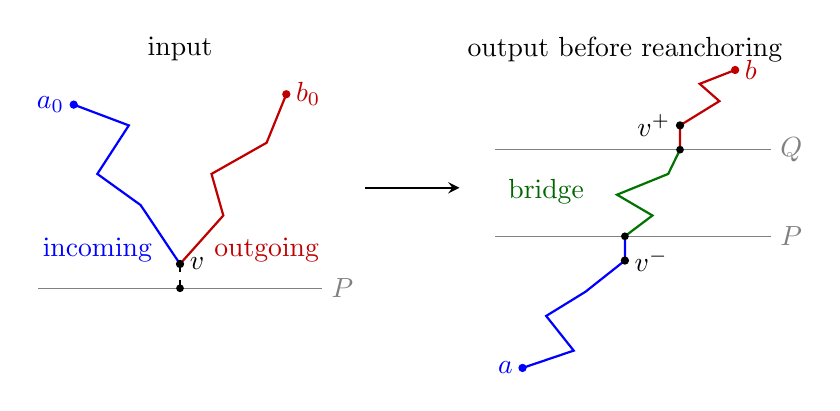
\begin{tikzpicture}[x=1cm,y=.88cm,>=stealth]
 \begin{scope}[xshift=-3.4cm]
  \node at (0,3.45) {input};
  \draw[gray] (-1.8,0)--(1.8,0) node[right] {$P$};
  \draw[thick,blue] (-1.35,2.65)--(-.65,2.35)--(-1.05,1.65)
    --(-.5,1.2)--(0,.35);
  \draw[thick,red!75!black] (0,.35)--(.55,1.05)--(.4,1.65)
    --(1.1,2.1)--(1.35,2.8);
  \draw[dashed] (0,0)--(0,.35);
  \fill (0,0) circle(1.4pt);
  \fill (0,.35) circle(1.5pt) node[right] {$v$};
  \fill[blue] (-1.35,2.65) circle(1.5pt) node[left] {$a_0$};
  \fill[red!75!black] (1.35,2.8) circle(1.5pt) node[right] {$b_0$};
  \node[blue] at (-1.05,.55) {incoming};
  \node[red!75!black] at (1.1,.55) {outgoing};
 \end{scope}
 \draw[->,thick] (-1.05,1.45)--(.15,1.45);
 \begin{scope}[xshift=2.25cm]
  \node at (0,3.45) {output before reanchoring};
  \draw[gray] (-1.65,.75)--(1.85,.75) node[right] {$P$};
  \draw[gray] (-1.65,2)--(1.85,2) node[right] {$Q$};
  \draw[thick,blue] (-1.3,-1.15)--(-.65,-.9)--(-1,-.4)
    --(-.5,-.05)--(0,.4)--(0,.75);
  \draw[thick,green!45!black] (0,.75)--(.35,1.05)
    --(-.1,1.35)--(.55,1.65)--(.7,2);
  \draw[thick,red!75!black] (.7,2)--(.7,2.35)--(1.2,2.7)
    --(.95,2.95)--(1.4,3.15);
  \fill (0,.75) circle(1.4pt);
  \fill (.7,2) circle(1.4pt);
  \fill (0,.4) circle(1.5pt) node[right] {$v^-$};
  \fill (.7,2.35) circle(1.5pt) node[left] {$v^+$};
  \fill[blue] (-1.3,-1.15) circle(1.5pt) node[left] {$a$};
  \fill[red!75!black] (1.4,3.15) circle(1.5pt) node[right] {$b$};
  \node[green!40!black] at (-1,1.4) {bridge};
 \end{scope}
\end{tikzpicture}
\caption{Insertion at an internal minimum, shown schematically rather
than as a lattice embedding. Reflect the blue incoming arm across $P$;
translate the red outgoing arm by the port increment of the green
bridge. The two copies $v^-,v^+$ of the minimum lie outside the inserted
slab. The walls $P,Q$ are global up-cuts of the output. Cutting there
and reversing these operations recovers the input. The final common
translation to fix the output root does not change
$P+Q-y(a)-y(b)$.}
\label{R:cal:refolding-figure}
\end{figure}

Both $P$ and $Q$ are global up-cuts of the output: each is crossed
exactly once, with all earlier vertices below and all later vertices
above. For fixed sign and cut levels, the inverse is unique. Cut at the
two ports, reflect the lower exterior back, translate the upper exterior
to align the ports, merge the two copies of $v$, and anchor the original
start. A pair is called \emph{valid} if this refolded walk is simple.
It need not satisfy the deterministic rule used to choose the input
minimum; counting all valid pairs only enlarges the inverse multiplicity.
If the input has absolute endpoint-height increment at most $r$, then
\begin{equation}
 |P+Q-y({\rm start})-y({\rm end})|\le r.
 \label{R:cal:refolding-displacement}
\end{equation}
Indeed before reanchoring the two output endpoint heights are
$2P-y(a_0)$ and $y(b_0)+Q-P$, and the expression is translation invariant.

\paragraph{Two bounds on the inverse labels.}
For ordered disjoint level intervals $I,J$, let $M_{I,J}(\omega)$ be
the number of valid pairs $(P,Q)$ of an output $\omega$ with
$P\in I$, $Q\in J$. The first bound below controls this count in one
pair of intervals. The second also bounds how many opposite interval
pairs can contain any cuts when \eqref{R:cal:refolding-displacement}
holds.

\begin{lemma}[Recoverable insertion labels]\label{R:cal:refolding-labels}
Fix $\eta>0$ and consider outputs of edge length at most $N^2$.
Each assertion below holds outside a family of total critical mass at
most $\exp(-N^c)$, for some $c>0$.
\begin{itemize}
\item If $I$ lies below $J$ and both have size at most $CH$, where
$1\le H\le CN^2$, then $M_{I,J}\le H^aN^\eta$.
\item Among valid pairs satisfying
\eqref{R:cal:refolding-displacement} and $s\le Q-P\le2s$, with
$1\le r\ll s\le CN^2$ and $s/r\to\infty$, there are at most
$Cs^a(r/s)^\vartheta N^{2\eta}$ pairs.
\end{itemize}
The exceptional-mass conclusion is preserved by polynomially many
choices of intervals, coordinates, and tests, and by any polynomial
multiplicity.
\end{lemma}
\begin{proof}
\textit{Valid pairs in fixed bins: the occurrence moment.}
Set $k=\lfloor N^\gamma\rfloor$, with $\gamma>0$ to be chosen small.
We bound the unnormalized occurrence moment
\[
 \sum_{\omega:\,|\omega|\le N^2}
       \rho^{|\omega|}M_{I,J}(\omega)^k,
\]
where $|\omega|$ is edge length and the output start is fixed. Expanding
the power selects an ordered tuple of $k$ valid pairs. Suppose it uses
$t$ distinct lower levels and $u$ distinct upper levels. Their incidence
pattern costs $\exp(O(k\log k))$. The lowest and highest levels have
polynomially many choices. The two exterior pieces cost at most
$CV_{CN^2}^2$: sum the first from the anchored source and the last freely
from its joining port. Every intervening segment is a strict bridge with
free transverse increment. The bridge between the last lower and first
upper cut has mass at most $\sup_h B_h\le C$.

The incidence graph has $t+u$ vertices and $k$ edges, hence at least
$t+u-k$ connected components. One edge from each component gives a
matching. Remove edges incident to the lowest lower or highest upper
level, leaving at least $t+u-k-2$ matches. For each retained match select
the gap immediately below its lower cut and the gap immediately above
its upper cut. All selected gaps are distinct. Bin the $t+u-2$
within-interval gap heights dyadically, at cost at most
$(C\log N)^{2k}$. An untested gap of scale $D$ costs
$\sum_{h\asymp D}B_h\le CD^a$.

\paragraph{Changing the measure on a selected gap.}
For matched gap scales $D_1,D_2$, choose
$g=\max(1,\lfloor\min(D_1,D_2)/4\rfloor)$ using the dyadic lower
ends. Read the lower gap backward from its upper cut and the upper gap
forward from its lower cut, reflecting to a common upward orientation.
Retain only complete irreducibles ending below $g$. For a relative
history $\xi$ of height $b<g$, write $\mu(\xi)=\rho^{L(\xi)}$.
Its censored-law probability is
\[
 P_g(\xi)=\mu(\xi)T(g-b),\qquad T(v)=p(H\ge v).
\]
Relative to this probability law, the summed weight of a gap of scale
$D$ has remaining kernel
\[
 K_D(\xi)=\mathbb E\left[
       \sum_{h\text{ in the gap bin}}B_{h-b-H}
       \,\middle|\,H\ge g-b\right]\le CD^a,
\]
with negative residual heights contributing zero. The crossing jump is
the first omitted irreducible. Renewal factorization proves the kernel
identity, and the bound is uniform in the retained history: for each
crossing jump the residual heights range over an interval of size
$O(D)$, whose bridge masses sum to at most $CD^a$.

Validity forces the two aligned histories to satisfy
\eqref{R:cal:survival-bound}, for one of the two assignments of roles.
They emanate from the same port and center and then follow disjoint
arms of the refolded walk. For a lower tested left cut $d_1$ and a
higher right cut $d_2<g$, continue the left arm to $d_2$, still inside
its selected gap. This is a strip crosscut with a unique crossing at
$d_1$, so every right-prefix crossing there lies to its right.

We now sum fine gap heights at fixed relative histories. The central
bridge was bounded uniformly, so these heights can be summed freely.
There is no transverse matching factor: translation to the next port
determines each placement, and the pair constraints use aligned relative
histories. Thus the occurrence sum is bounded by an integral under
independent censored reference laws, with kernels bounded by $CD_i^a$.
It does not require independence under the law of an output conditioned
on its labels. Distinct matches use disjoint gaps, so the survival costs
multiply. Each match contributes at most
\[
 C_\theta D_1^aD_2^a g^{-a+\theta}
       \le C'_\theta H^aN^{3\theta}.
\]
There are $t+u-2$ gaps and at least $t+u-k-2$ such savings. Including
untested gaps and all classifications therefore gives
\[
 \sum_{\omega:\,|\omega|\le N^2}
       \rho^{|\omega|}M_{I,J}(\omega)^k
 \le N^{O(1)}V_{CN^2}^2 H^{ak}N^{3\theta k}
       \exp\{O_\theta(k\log(k\log N))\}.
\]
Choose $\theta$, then $\gamma$, sufficiently small relative to $\eta$,
and use \eqref{R:cal:volume-bound} with $2\nu<\gamma$. Markov's
inequality at $H^aN^\eta$ proves the first exceptional-mass bound.

\paragraph{How many opposite bins contain cuts?}
Fix the output terminal height at polynomial cost and put
$T=y({\rm start})+y({\rm end})$. Under the displacement constraint,
$P$ ranges over an interval of size $O(s)$ below $T/2$ by at least
$(s-r)/2$. Partition this range into intervals $I_i$ of width $r$.
The possible partners lie in $J_i=T-I_i+[-r,r]$, above all the lower
bins for large $s/r$. There are $L'\le Cs/r$ bins. The first part of
the lemma bounds valid pairs in each $(I_i,J_i)$ by $Cr^aN^\eta$.
It remains to count occupied bins, meaning bins with some global
up-cut in each interval, without requiring that the pair be valid.

Separate the indices into a fixed number of residue classes, say
modulo ten. Test $k$ increasing occupied indices in one class. The
upper intervals occur in reverse order, and a gap of $d$ indices
corresponds to height separation comparable to $dr$ on both sides.
Fix the outermost two cut levels at polynomial cost. From each end
of the bridge between them, stop successively at the first renewal
hit in the next required interval. A hit in an interval of width
$O(r)$ at distance comparable to $dr$ has probability at most
$Cd^{-\vartheta}$. Indeed, after its first hit the expected number
of renewals in the next $r$ levels is
$\sum_{j\le r}B_j\gtrsim r^a$, while the unconditional expected number
in the enlarged interval is at most $Cr(dr)^{-\vartheta}$.

These costs multiply over successive first hits. The two prefixes
stop at separated levels; their remaining joining bridge costs at
most $C$. The reverse prefix at the upper end is placed by translation,
with its outer transverse port free. Hence the two sides together
cost $Cd^{-2\vartheta}$ per index gap. Summing the gaps gives
\[
 \sum_{d\le L'}Cd^{-2\vartheta}\le C(s/r)^{1-2\vartheta}.
\]
If $Y$ counts occupied bins in this residue class, its weighted
binomial moment is consequently at most
\[
 \sum_{\omega:\,|\omega|\le N^2}\rho^{|\omega|}\binom{Y(\omega)}k
 \le N^{O(1)}V_{CN^2}^2
        \bigl(C(s/r)^{1-2\vartheta}\bigr)^k.
\]
Take $k=\lfloor N^\gamma\rfloor$ with $\gamma$ sufficiently small
relative to $\eta$. The binomial Markov estimate, including its factor
$k^k$, bounds $Y$ by $C(s/r)^{1-2\vartheta}N^\eta$ outside a
stretched-exponential exceptional mass. Multiply this by the first
bound per bin. Since $a=1-\vartheta$, the result is
\[
 Cr^a(s/r)^{1-2\vartheta}N^{2\eta}
       =Cs^a(r/s)^\vartheta N^{2\eta},
\]
which proves the second bound. All coordinates and labels have
polynomial ranges for outputs of length at most $N^2$, so the stated
unions and multiplicities preserve both exception estimates.
\end{proof}

\begin{proof}[Proof of Theorem~\ref{R:cal:plane-laws}]
\textit{Comparing short-displacement and total masses.}
Fix a small $\epsilon>0$ and a dyad $[N,2N)$. Choose fixed positive
$\zeta,\eta$ sufficiently small relative to $\epsilon$, and put
\[
 r=N^{3/4-\epsilon/2},\qquad
 s=N^{3/4-\zeta},\qquad R=N^{3/4+\zeta}.
\]
Let $b_j$ be the critical mass of eligible $j$-edge inputs whose absolute
endpoint-height increment is at most $r$. Choose $l$ with probability
$A_l/A$, independently of $n$, and set $j=n-l-1$. The insertion outputs
at length $n$, counted with multiplicity, have mass
$\rho\sum_l A_l b_j$. The second label bound and $A\asymp s^a$ give
\[
 \mathbb E_l[b_j/c_n]\le C(r/s)^\vartheta N^{2\eta}.
\]
The exceptional outputs contribute negligibly: their absolute mass is
stretched-exponentially small, their multiplicity is polynomial, and
$c_n\ge1$.

For comparison, restrict all eligible inputs to diameter at most $R$.
They retain $(1-o(1))c_j$ mass uniformly in the relevant lengths, by
the fast-path bound and the $o(1)$ omitted mass. Their lower cut $P$
lies within $CR$ of the output starting height. Cover this range by
$O(1+R/s)$ intervals of size at most $s/10$; each has an associated
higher interval of size $O(s)$ for $Q$. The first label bound gives
multiplicity at most $C(1+R/s)s^aN^\eta$. After dividing by $A$,
\[
 \mathbb E_l[c_j/c_n]\le CN^{2\zeta+\eta}.
\]

\paragraph{The logarithmic comparison and its boundary error.}
Put $\kappa=\vartheta/8$. Jensen's inequality applied to the sum of
the two mass ratios gives
\begin{align*}
 &\mathbb E_l\log(1+N^{\kappa\epsilon}b_j/c_j)
       +\mathbb E_l\log(c_j/c_n)\\
 &\hspace{1cm}\le
       \log\mathbb E_l[(c_j+N^{\kappa\epsilon}b_j)/c_n]
       \le(2\zeta+\eta+o(1))\log N.
\end{align*}
For the last inequality it suffices, for example, to choose
$\vartheta\zeta+2\eta<3\vartheta\epsilon/8$; the scaled short-displacement
term then even tends to zero. We have obtained
\[
 \mathbb E_l\log(1+N^{\kappa\epsilon}b_j/c_j)
 \le(2\zeta+\eta+o(1))\log N
       +\log c_n-\mathbb E_l\log c_j.
\]
The maximal shift is
\[
 D_N:=\max(l+1)=O(s^{d_*})=O(N^{1-4\zeta/3})=o(N).
\]
For each fixed shift, summing the last difference over $N\le n<2N$
cancels all interior terms. The volume bound leaves boundary error
\[
 O_\nu(D_NN^\nu)=o(N),\qquad 0<\nu<4\zeta/3.
\]
The left summand is between zero and $O(\log N)$ because $b_j\le c_j$.
Reindexing it from $j=n-l-1$ to the exact dyad therefore costs at most
$O(D_N\log N)=o(N)$. For each fixed $\lambda>0$, it follows that
\[
 \limsup_{N\to\infty}\frac1N
 \#\{N\le n<2N:b_n/c_n>\lambda\}
 \le\frac{2\zeta+\eta}{\kappa\epsilon}.
\]
Here $b_n$ depends on $N,\epsilon$, but not on $\zeta,\eta$. Keep all
parameters fixed while taking this limit, and then let $\zeta,\eta$
tend to zero. The upper fraction is zero.

\paragraph{One set of lengths for probability and moments.}
Adding back the omitted walks changes the probability by $o(1)$,
since $c_n\ge1$. Thus the lower cutoff $n^{3/4-\epsilon}$ holds for
absolute normal displacement outside a vanishing fraction of each
dyad. As in the half-plane argument, let the slacks and probability-error
thresholds decrease sufficiently slowly over dyads. The retained lengths
have natural density one. Intersecting with the half-plane set retains
natural density one and gives a common set for both laws. Endpoint
distance dominates normal displacement,
and the all-length upper tail already controls maximum radius. This
proves both probability exponents. The same lower cutoff and the
superpolynomial upper tail, with the deterministic linear bound, give
the moments for every fixed $p>0$ on that one set.

\paragraph{An alternative full-plane thermal proof.}
The same insertion gives the thermal conclusion by the calibrated and
censored estimates, independently of the reserved-height comparison in
Section~\ref{R:sec:thermal}. Take $N=\lceil1/t\rceil$ and the same
$r,s$. The partition sum $Z(t)=\sum_m c_me^{-tm}$ is at least $cN$.
The volume bound makes lengths $m>N^{1+\delta}$ superpolynomially
unlikely, also with any fixed length power, for each fixed small
$\delta>0$. Insert into eligible short-displacement inputs below this
cutoff. Outputs have length at most $N^2$, and
$e^{-t(l+1)}=1-o(1)$ uniformly since $l+1=o(N)$. The second label
bound, now summed with thermal weights, gives
\[
 \sum_{m\le N^{1+\delta}}b_me^{-tm}
 \le C(r/s)^\vartheta N^{2\eta}Z(t).
\]
The omitted walks have $o(1)$ mass at each large exact length, so their
thermal mass is $o(N)$. This proves the endpoint lower cutoff at every
large discount scale. The uniform speed bound, conditioned on lengths
between $N^{1/2}$ and $N^{1+\delta}$, gives the spatial upper cutoff
and its moments. Smaller lengths are atypical by the endpoint lower
cutoff. Finally the same lower cutoff and speed bound give the typical
length lower power; the volume bound gives its upper tail and all
positive length moments.
\end{proof}

\subsection{An independent count of favorable exact lengths}
\label{R:cal:good-lengths}
The density-one theorem is stronger than a power-cardinality conclusion,
but uses censored survival and refolding. We record a separate consequence
of the thermal route under its weaker length precision: the deficit
$1-\mathbb E e^{-L/N}=N^{-\alpha+o(1)}$, the absolute mass and upper
spatial estimates, and the turning-chain bound with a reserved independent
group. No insertion-label bound is needed. The additional ingredient is a
length atom estimate on that reserved group.

\begin{proposition}[Power-cardinality of favorable lengths]
\label{R:cal:good-cardinality}
Fix $0<\epsilon<1$. For unrestricted uniform honeycomb walks rooted at a
fixed center, the number of integers $m\in[R^{1-\epsilon},R]$ for which
\[
 \Pr_m\{m^{3/4-\epsilon}\le |\omega_m-\omega_0|
       \le\operatorname{diam}(\omega)\le m^{3/4+\epsilon}\}
       \ge1-\epsilon
\]
is $R^{1+o(1)}$ as $R\to\infty$. In particular, the limsup of each positive
moment exponent of endpoint distance or diameter is $3/4$ times its moment
order. If the corresponding spatial exponent in probability exists at all
exact lengths, it equals $3/4$.
\end{proposition}
\begin{proof}
Write $\alpha=9/16$. We first record the length atom estimate under the
exponent-precision hypotheses of the turning-chain route. If the length
$L$ of one irreducible satisfies
$1-\mathbb E e^{-L/r}=r^{-\alpha+o(1)}$, then independent sums satisfy
\begin{equation}
 \sup_m p(S_L(j)=m)\le j^{-1/\alpha+o(1)}.
 \label{R:cal:exponent-length-atom}
\end{equation}
Here is a direct verification, without logarithmic precision. Fix a small
$\zeta>0$ and put $z=r^{1-\zeta/2}$. The Laplace estimate implies
$p(L>s)\le s^{-\alpha+o(1)}$ and
$\mathbb E[L;L\le s]\le s^{1-\alpha+o(1)}$. Hence the contributions of
$L<r^{1-\zeta}$ and $L>r/10$ to
$\mathbb E(1-e^{-L/z})$ are negligible compared with $z^{-\alpha+o(1)}$.
The intermediate interval therefore has probability at least
$r^{-(1-\zeta/2)\alpha+o(1)}$. Subtracting an independent bounded-length
copy in the characteristic-function symmetrization gives phases between
$c r^{-\zeta}$ and a fixed constant below $\pi$ at frequency $1/r$.
Thus the squared characteristic-function modulus is at most
$1-c r^{-\alpha-O(\zeta)+o(1)}$. On the actual length lattice all
modulus-one characters form a finite set and translate the same bound.
Fourier inversion, followed by $\zeta\downarrow0$, proves
\eqref{R:cal:exponent-length-atom}.

Now take the full-plane thermal law with edge weights
$(\rho e^{-1/N})^m$ and its deterministic minimum-split decomposition.
Use the notation of the two-end estimate in
Corollary~\ref{R:geo:two-ends}: for a height scale $H_i$ and count scale
$k_i$, let $K_i=H_i^{3/4}$ and $\kappa_i=\min(k_i,K_i)$. Put
$M=\max_i\kappa_i$ on the nonempty bridges, and $M=1$ if there are none.
The endpoint-minimum case is included using its one-end decomposition.
Restrict to length at most $N^2$, whose complement has negligible thermal
probability by the absolute critical mass bound.

The turning-chain estimate without smoothing bounds the critical mass of
each dyadic family, including count choices, by $MN^{o(1)}$. The two
no-renewal ends cost at most a constant times $U_N^2$. Lemma~\ref{R:thermal:denominator} bounds the plane
normalization below by
$(q_N^{-1}-1)U_N^2$, where $q_N=N^{-\alpha+o(1)}$. Consequently all
families with $M<N^{\alpha-\eta}$ have vanishing normalized mass, for every
fixed $\eta>0$.

In the remaining families fix the end shapes, all witness labels, and all
pieces except the unused batch belonging to an index attaining $M$.
Proposition~\ref{R:geo:chain} reserves this batch independently of the
avoidance tests and the large-height and short-length tests. Exact total
length is therefore one scalar equality in that batch. Applying
\eqref{R:cal:exponent-length-atom} costs an additional
$M^{-1/\alpha+o(1)}$, uniformly in the fixed outside data. The bounded
endpoint length corrections merely change the target integer. Damping may
be dropped on these bridges before using the critical estimate. After
normalization, for every integer $m$ the mass of length $m$ in the retained
families is at most
\[
 N^{-\alpha+o(1)}M^{1-1/\alpha}
 \le N^{-1+(1/\alpha-1)\eta+o(1)}.
\]
No independence between the length and height of an individual irreducible
is used: its entire batch remains unexposed until this scalar test.

Theorem~\ref{R:thermal:law} gives probability tending to one
to $N^{1-s}\le m\le N^{1+s}$ and to the corresponding spatial exponent
window with fixed slack $s>0$. Conditional on $m$, the thermal law is the
uniform law. Taking $s$ sufficiently small relative to $\epsilon$ and
using Markov's inequality on the conditional failure probability, the
lengths satisfying the proposition carry probability tending to one.
Their intersection with the retained families still does so. The uniform
atom bound forces their number to be at least
$N^{1-O(\eta)+o(1)}$.

Set $N=R^{1/(1+2s)}$. For small enough $s$ the resulting length interval
lies in $[R^{1-\epsilon},R]$. Since $s$ and $\eta$ are arbitrarily small,
the count is at least $R^{1-o(1)}$, and the trivial bound by $R$ proves the
claim. The limsup assertions combine these favorable lengths with the
all-length upper spatial tail. This argument gives power-cardinality;
the separate refolding argument establishes the density-one conclusion.
\end{proof}

\section{Correlation lengths, pulling, and prescribed spatial endpoints}
\label{R:resp:section}

There are two further ways to change the thermal law. One may reward displacement by an exponential factor, or prescribe the terminal vertex. The first change tests convergence of a generating function. The second asks for one coefficient in two spatial coordinates. We first determine the exponential threshold and the associated force response. We then prove the spatial local estimate needed to normalize a prescribed endpoint.

In this section lengths $\ell$ count edges of ordinary walks from a fixed vertex $o$. Put $z_t=\rho e^{-t}$, $t>0$, and define
\[
 G_t(b)=\sum_{\gamma:o\to b}z_t^{\ell(\gamma)},\qquad
 \chi(t)=\sum_bG_t(b).
\]
The empty walk is included. For a unit vector $e$, let
\begin{align}
 m_e(t)&=\sup\left\{s\ge0:\sum_b e^{s e\cdot(b-o)}G_t(b)<\infty\right\},
 \label{R:resp:directional-mass}\\
 m_{\mathrm{rad}}(t)&=\sup\left\{s\ge0:\sum_b e^{s|b-o|}G_t(b)<\infty\right\}.
 \label{R:resp:radial-mass}
\end{align}
Both convergence sets are intervals containing zero. For the directional sum this follows by separating nonnegative and negative projections; the latter contribution is bounded by $\chi(t)$. All constants below allow the fixed conversion between Euclidean units and row spacing.

Directional decay and endpoint tilts have long been studied through renewal methods. Ioffe proved all-direction Ornstein--Zernike asymptotics for self-avoiding walk on $\mathbb Z^d$ in the strictly subcritical fugacity regime~\cite{Ioffe1998}. Borgs, Chayes, King and Madras studied directional masses for anisotropic walks and linear displacement of the most likely endpoint under asymmetric positive step weights~\cite{BorgsChayesKingMadras2000}. Ioffe and Velenik proved ballistic local limit results for self-interacting walks under fixed forces in the ballistic regime~\cite{IoffeVelenik2008}. Our estimates concern the approach to zero force and critical fugacity on the honeycomb lattice. We derive the required uniform powers from the quantitative bridge estimates above.

\begin{theorem}[Exponential thresholds and force]\label{R:resp:force}
Uniformly over unit vectors $e$, as $t\downarrow0$,
\[
 m_e(t)=t^{3/4+o(1)},\qquad m_{\mathrm{rad}}(t)=t^{3/4+o(1)}.
\]
More precisely, for every $\varepsilon>0$ and all sufficiently small $t$,
\[
 t^{3/4+\varepsilon}\le m_{\mathrm{rad}}(t)\le m_e(t)\le C t^{3/4},
\]
where $C$ is independent of $e$. For each unit vector $e$ and $s\ge0$, the limit
\[
 f_e(s)=\lim_{j\to\infty}\frac1j\log
 \sum_{\ell(\gamma)=j}\rho^j e^{s e\cdot(\gamma_j-o)}
\]
exists. It satisfies $f_e(0)=0$ and
\[
 f_e(s)=s^{4/3+o(1)}\qquad(s\downarrow0),
\]
uniformly in $e$.
\end{theorem}

The proof uses two consequences of the absolute count and fast-path bounds in Propositions~\ref{R:geo:absolute-count} and~\ref{R:geo:fast}. For every fixed sufficiently small $\xi>0$,
\begin{equation}
 \sum_{\substack{R\le D(\gamma)\le2R\\ L(\gamma)\le R^{4/3-\xi}}}
       \rho^{L(\gamma)}\le C_\xi e^{-R^{c_\xi}},
 \qquad
 U_R:=\sum_{D(\gamma)\le R}\rho^{L(\gamma)}
       \le e^{C_\nu(1+R)^\nu}\quad(\nu>0).
 \label{R:resp:critical-inputs}
\end{equation}
These sums start at a specified vertex and count vertices in $L$. For the first bound, paths of diameter at least $R$ have length at least $cR$. Choose $\eta>0$ so small that $(4/3-\xi)(3/4+\eta)<1$. At each remaining length $n\le R^{4/3-\xi}$, the refined fast-path estimate applies and gives mass at most
\[
 \exp(-c_\eta R/n^{3/4})\le\exp(-c_\eta R^{3\xi/4}).
\]
Summing the polynomial number of lengths gives the first bound. For the second, a self-avoiding trace of diameter at most $R$ visits at most $C(1+R)^2$ lattice vertices. Apply the absolute count bound with exponent smaller than $\nu/2$ and sum over these lengths. Changing either sum to edge weights costs one constant factor.

For the divergence estimate we need a positive mass of bridges whose thermal discount is bounded below. Theorem~\ref{R:renew:finite-input} gives $B_h\ge ch^{-1/4}$ and $M_h\le Ch^{13/12}$. Hence
\[
 B_h\{L>C_0h^{4/3}\}\le \frac{M_h}{C_0h^{4/3}}
       \le \frac C{C_0}h^{-1/4}.
\]
Choosing the fixed $C_0$ large enough retains a positive fraction of $B_h$ with $L\le C_0h^{4/3}$. This uses the finite first-length mass before any exact-length conditioning.

\begin{proof}[Proof of Theorem~\ref{R:resp:force}]
Fix $\varepsilon>0$ and put $R=t^{-3/4-\varepsilon}$. Stop a walk on its first visit to distance at least $R$ from its starting vertex. Its endpoint lies at distance at most $R+a_{\mathrm{lat}}$, where $a_{\mathrm{lat}}$ is the lattice edge length, and its diameter lies between $R$ and $2R+a_{\mathrm{lat}}$. Let $W(t,R)$ be the total $z_t$-weight of these stopped prefixes. The prefixes with at most $R^{4/3-\xi}$ vertices have mass tending to zero by the first estimate in~\eqref{R:resp:critical-inputs}, with harmless fixed adjustments of the radii. The remaining prefixes have total mass at most
\[
 C U_{3R}\exp(-tR^{4/3-\xi}).
\]
Choose $\xi>0$ so small that
\[
 4/3-\xi-\frac1{3/4+\varepsilon}>0,
\]
and then choose $\nu$ smaller than this difference in the bound for $U_{3R}$. It follows that $W(t,R)=o(1)$.

Now split any complete walk greedily into such stopped prefixes, restarting the rule at the endpoint of each prefix, followed by one remainder whose displacement is less than $R$. Edge weights multiply. Dropping avoidance between different pieces gives, at $s=1/R$,
\[
 \sum_\gamma z_t^{\ell(\gamma)}e^{sA(\gamma)}
 \le e\chi(t)\sum_{k\ge0}
       \bigl(e^{1+a_{\mathrm{lat}}/R}\max_{\text{vertex types}}W(t,R)\bigr)^k<\infty
\]
for all sufficiently small $t$. The estimates hold at both vertex types by lattice symmetry. Thus $m_{\mathrm{rad}}(t)\ge t^{3/4+\varepsilon}$, and $m_e(t)\ge m_{\mathrm{rad}}(t)$.

To prove divergence, take an integer height $H\asymp t^{-3/4}$. Choose one of the three inward port normals at $o$ whose scalar product with $e$ is at least $1/2$. Consider bridges in that direction with height $h\in[H,2H]$, length at most $C_1H^{4/3}$, and horizontal displacement of the sign favorable to $e$. Reflection in the normal preserves length and critical weight, so the total mass at every such height is at least $cH^{-1/4}$. Every retained displacement has projection on $e$ at least $c_0H$, where $c_0>0$ is independent of $e$.

From each retained bridge extract the prefix ending at its first renewal cut whose relative height lies in $[H,2H]$ and whose prefix has the stated sign and length properties. Such a cut exists because the terminal cut qualifies. A fixed extracted prefix may have suffixes to several heights in $[H,2H]$; their total critical mass is at most
\[
 \sum_{0\le j\le H}B_j\le CH^{3/4}.
\]
Since the original bridges summed over heights have mass at least $cH^{3/4}$, the distinct extracted prefixes have total critical mass at least a fixed $c_1>0$. Their lengths are at most $C_1H^{4/3}$, so their $e^{-tL}$-discounted mass is also bounded below by a fixed positive constant.

Concatenate any number of these prefixes in the chosen direction. The pieces lie in successive disjoint open slabs. Their joins are recoverable by the same first-qualifying-cut rule, relative to the current initial port. Later pieces cannot change an earlier cut or its prefix tests. Hence different ordered lists give different port paths. Trimming the initial and final half-edges gives ordinary plane walks from $o$; the length and endpoint-weight corrections are bounded independently of the number of pieces. Consequently the directionally tilted plane sum diverges when
\[
 c_2e^{s c_0H}>1.
\]
This proves $m_e(t)\le C/H\le Ct^{3/4}$, uniformly in $e$.

It remains to pass from convergence thresholds to the fixed-length free energy. Write
\[
 a_j(s,e)=\sum_{\ell(\gamma)=j}\rho^j
             e^{s e\cdot(\gamma_j-o)}.
\]
After an even number of steps the terminal vertex has the same lattice type as $o$. Splitting there and dropping avoidance therefore gives
$a_{2j+2k}\le a_{2j}a_{2k}$. Fekete's lemma gives a limit for $(2j)^{-1}\log a_{2j}$. Single-edge truncation gives
\[
 a_{j+1}\le 3\rho e^{s a_{\mathrm{lat}}}a_j.
\]
Applying this twice places each odd-length logarithm between the adjacent even-length logarithms up to a constant. Thus the limit defining $f_e(s)$ exists at all lengths. It is finite. The connective-constant identity gives $f_e(0)=0$.

The directional susceptibility is $\sum_j e^{-tj}a_j(s,e)$. The root test shows that it converges if $t>f_e(s)$ and diverges if $t<f_e(s)$. In particular, $s<m_e(t)$ implies $f_e(s)\le t$, and $s>m_e(t)$ implies $f_e(s)\ge t$. Applying the threshold bounds with $t=s^{1/(3/4+\delta)}$ and $t=s^{1/(3/4-\delta)}$, with an arbitrarily small fixed $\delta>0$ and harmless constant adjustments, proves $f_e(s)=s^{4/3+o(1)}$. All threshold constants used here are uniform in $e$.
\end{proof}

\begin{corollary}[One-sided force response]\label{R:resp:force-derivatives}
For $s>0$ the convex function $f_e$ has one-sided derivatives, and
\[
 f'_{e,-}(s)=s^{1/3+o(1)},\qquad f'_{e,+}(s)=s^{1/3+o(1)}
 \qquad(s\downarrow0).
\]
At a point where $f_e$ is differentiable, the mean displacement in direction $e$, divided by length, under the force-weighted $j$-edge law tends to $f'_e(s)$ as $j\to\infty$.
\end{corollary}
\begin{proof}
Each $j^{-1}\log a_j(s,e)$ is convex, and its pointwise limit is convex. Since $f_e(0)=0$, convexity gives
\[
 \frac{f_e(s)}s\le f'_{e,-}(s)\le f'_{e,+}(s)
       \le\frac{f_e(2s)-f_e(s)}s\le\frac{f_e(2s)}s.
\]
Here $f_e(s)\ge0$: rotation by $120$ degrees about $o$ makes the mean endpoint of the unforced fixed-length law zero, so Jensen's inequality gives $a_j(s,e)\ge a_j(0,e)$. Theorem~\ref{R:resp:force} now proves the derivative exponents. Finally the derivative of $j^{-1}\log a_j$ is the stated normalized mean. Its lower and upper difference quotients converge to those of $f_e$; letting their increments tend to zero proves the claim at differentiability points. No differentiability assertion is needed for the one-sided result.
\end{proof}

The exponent $1/3$ agrees with Pincus's force-extension scaling relation $1/\nu-1$ at $\nu=3/4$~\cite[Eq.~(I.4)]{Pincus1976}; here it follows from the threshold bounds and convexity. This small-force relation is distinct from fixed-force ballistic asymptotics; see also~\cite[Section~4.2.3]{IoffeVelenik2010}.

For prescribed endpoints we will use the same geometric estimates before summing over lengths. In edge-count notation, the absolute critical count bound in Proposition~\ref{R:geo:absolute-count} is
$c_j\rho^j\le\exp(C_\nu j^\nu)$ for every $\nu>0$, where $c_j$ counts rooted $j$-edge walks. The refined fast-path bound in Proposition~\ref{R:geo:fast} is
\begin{equation}
 \sum_{\substack{\ell(\gamma)=j\\D(\gamma)\ge d}}\rho^j
       \le\exp\bigl(-c_\eta d/j^{3/4}\bigr),
 \qquad d\ge j^{3/4+\eta},
 \label{R:resp:refined-fast}
\end{equation}
for fixed $\eta>0$ and sufficiently large $j$. The conversion from vertex count to edge count changes length by one and weight by a fixed factor; decreasing the slack and the exponential constant absorbs both changes. Both bounds concern unnormalized masses, so they remain available before a prescribed endpoint has been normalized.

\begin{remark}[A second route to the radial threshold]\label{R:resp:radial-alternative}
The turning-chain estimates give a useful alternative which requires no first-length estimate at a single chosen height. Write $p$ for the critical irreducible law, $T$ for its height and $L$ for its vertex length. By Lemma~\ref{R:geo:increment-tails} and the length deficit in Proposition~\ref{R:renew:increments},
\[
 p(e^{-L/N};T>R)\ge cR^{-3/4}-q_N,
 \qquad q_N:=p(1-e^{-L/N})=N^{-9/16+o(1)}.
\]
At $R=N^{3/4-\delta}$ the right side is at least $c'R^{-3/4}$. A pull $s=N^{-3/4+2\delta}$ in a fixed positive multiple of the height therefore makes the total tilted irreducible weight exceed one. Free concatenation then forces divergence of the radially tilted plane sum, after the bounded endpoint conversion.

For convergence put $s=N^{-3/4-\delta}$ and choose an even block length $j\asymp N^{1+\eta}$ with $\eta$ sufficiently small after $\delta$. On $D\le j^{3/4+\eta}$ the pull is bounded, while $e^{-j/N}$ beats the critical count bound. On successive larger diameter ranges, \eqref{R:resp:refined-fast} beats the pull because $s\ll j^{-3/4}$. The tilted mass of this block is less than one at both vertex types. Splitting paths into such blocks, with one bounded-length remainder, proves convergence. This recovers $m_{\mathrm{rad}}(1/N)=N^{-3/4+o(1)}$ by an argument directly adapted to the absolute turning-chain bounds.
\end{remark}

\subsection{A spatial local limit with lattice compatibility}
The exponential threshold alone gives no lower bound for $G_t(b)$ at a specified vertex. We now prove that a sum of order $H^{3/4}$ irreducible bridges can reach every admissible target of height $H$ at the expected two-dimensional lattice scale. The proof does not assume convergence to a unique stable law.

Let $Y=(T,X)$ be the displacement of one $p$-distributed irreducible, with $T$ measured in row spacings and $X$ in units of the spacing between ports on one cut. The ports on row $h$ are shifted horizontally by $h/2$ modulo this spacing. Thus their relative-displacement lattice is
\[
 \Gamma=\{(h,m+h/2):h,m\in\mathbb Z\}.
\]
The two elementary two-vertex bridges have displacements $(1,1/2)$ and $(1,-1/2)$. They are irreducible and generate $\Gamma$, so $\Gamma$ is also the lattice generated by all possible increments. Let $\Delta$ be the Euclidean diameter of an irreducible and $L$ its vertex length. Put $\beta=3/4$ and $K=H^\beta$.

For Fourier inversion the relevant subgroup is $\Gamma_1$, generated by differences of possible increments. Lemma~\ref{R:geo:atoms} proves that $\Gamma_1$ has rank two and hence finite index in $\Gamma$. All increments have one common class $a_*+\Gamma_1$; that class generates $\Gamma/\Gamma_1$. We call $k$ compatible with $y\in\Gamma$ when $ka_*-y\in\Gamma_1$.

\begin{proposition}[Prescribed displacement with controlled length and diameter]
\label{R:resp:point-local}
For each $C<\infty$ and $\eta>0$ there are $c>0$, $M_0<\infty$ and $H_0<\infty$ such that, for every integer $H\ge H_0$ and relative-port target $y=(H,x)\in\Gamma$ with $|x|\le CH$,
\begin{equation}
 \sum_{\lceil K\rceil\le k\le\lfloor2K\rfloor}
 p^{\otimes k}\left\{
 \sum_{i=1}^kY_i=y,\quad
 \sum_{i=1}^kL_i\le H^{4/3+\eta},\quad
 \sum_{i=1}^k\Delta_i\le M_0H
 \right\}
 \ge c K H^{-2}=cH^{-5/4}.
 \label{R:resp:point-bound}
\end{equation}
Incompatible counts contribute zero. In particular the paths counted here remain within distance $M_0H$ of their initial port.
\end{proposition}

\begin{proof}
We first establish the estimate without the length and diameter restrictions. Although subsequential laws of the rescaled sums may differ, each has full forward support and a strictly positive density in the open forward half-plane. Fourier inversion will then give a uniform lattice lower bound. Finally we mark individual increments to impose the two restrictions.

\emph{Subsequential jump limits.} Lemma~\ref{R:geo:increment-tails} gives
\begin{equation}
 p(|Y|>r)\le Cr^{-\beta},\qquad
 p(|Y|;|Y|\le r)\le Cr^{1-\beta}.
 \label{R:resp:jump-bounds}
\end{equation}
Consider any sequence $H\to\infty$. On a subsequence the measures
\[
 \mu_H=H^\beta p(Y/H\in\cdot)
\]
converge vaguely on $\mathbb R^2\setminus\{0\}$ to a measure $\mu$. This follows by compactness on each closed annulus and a diagonal extraction. The bounds
\[
 \mu_H(|y|>r)\le Cr^{-\beta},\qquad
 \int_{|y|\le r}|y|\,d\mu_H(y)\le Cr^{1-\beta}
\]
give the corresponding bounds for $\mu$, by approximation away from zero. In particular $\int(1\wedge|y|)\,d\mu(y)<\infty$. The measure is supported in $\{T\ge0\}$.

If $k/H^\beta\to u>0$, expansion of one characteristic function gives
\begin{equation}
 \mathbb E\exp\left(is\cdot H^{-1}\sum_{i=1}^kY_i\right)
 \longrightarrow
 F_u(s):=\exp\left(u\int(e^{is\cdot y}-1)\,d\mu(y)\right).
 \label{R:resp:poisson-transform}
\end{equation}
For completeness, truncate the integral to $\delta\le|y|\le M$. Vague convergence gives the limit there at continuity radii. The small-jump error is at most $C|s|\delta^{1-\beta}$; the large-jump error is at most $CM^{-\beta}$. Send first $H$ to infinity, then $\delta$ to zero and $M$ to infinity. The one-factor error is $O(H^{-\beta})$, so its squared term disappears after multiplication by $k$.

The right side is a characteristic function. Construct independent Poisson point collections on disjoint annuli, with intensity $u\mu$, and sum their points. There are finitely many points outside the unit disk, and the sum of the norms inside it has finite expectation. Thus the small-jump series converges absolutely almost surely. This is the finite-variation form of the Poisson construction of a pure-jump infinitely divisible law; see Schilling~\cite[Chapter~7]{Schilling2016} for the general construction. Tightness of the rescaled sums also follows directly from~\eqref{R:resp:jump-bounds}: remove jumps above $M$, and use the truncated first moment for the others. Fourier uniqueness therefore proves weak convergence to the constructed law. We prove the support and uniform lattice lower bound needed here next.

\emph{Full forward support.} For any $u>0$ the support of the limiting law is the closed additive semigroup generated by the support of $\mu$, including zero, and is independent of $u$. One inclusion follows by truncating the Poisson sum. Conversely, a specified finite list of jumps can be approximated with positive probability, excluding every other jump above a small cutoff. The remaining small jumps have arbitrarily small total norm with positive probability, by their first-moment bound. Hence each finite sum of support points belongs to the support.

This semigroup contains the entire open forward half-plane. To prove it, fix an open ball $B$ whose closure lies in $\{T>0\}$ and then a smaller closed ball $B'$ in $B$. The free-terminal guide estimate in Section~\ref{R:geo:finite-inputs}, applied over a fixed positive interval of target heights, gives
\begin{equation}
 \sum_{k\ge0}p^{*k}(HB')\ge c_B H^\beta.
 \label{R:resp:bridge-ball}
\end{equation}
Indeed a narrow straight guide places the terminal port in $HB'$, uniformly over order $H$ heights, and contributes $cH^{-1/4}$ at each height. Counts $k\le\xi H^\beta$ have total contribution at most $C_B\xi^2H^\beta$: to reach $HB'$ their height sum must exceed $c_BH$, and the truncated-sum bound from~\eqref{R:resp:jump-bounds} gives probability at most $C_B kH^{-\beta}$. Counts $k\ge S H^\beta$ contribute at most $C_BH^\beta e^{-c_BS}$, because
\[
 p\left(\sum_{i=1}^kT_i\le C_BH\right)
 \le e^{C_B}\bigl(p(e^{-T/H})\bigr)^k
 \le C_Be^{-c_B k/H^\beta}.
\]
Choose $\xi$ small and $S$ large. The remaining mass in~\eqref{R:resp:bridge-ball} is at least $c'_BH^\beta$, spread over at most $SH^\beta+1$ counts. Thus for some $k_H\in[\xi H^\beta,SH^\beta]$, the probability of $H^{-1}\sum_{i\le k_H}Y_i\in B'$ is bounded below independently of $H$. On a further subsequence $k_H/H^\beta\to u\in[\xi,S]$. Weak convergence and the closedness of $B'$ show that the limiting law gives positive mass to $B'$. Because all positive $u$ have the same support, every such ball meets the support of every limiting law.

\emph{Fourier inversion on the displacement lattice.} We have obtained full support in the open forward half-plane. To turn this into a positive lattice lower bound, we need a density and Fourier domination. Write $\varphi(\theta)=p(e^{i\theta\cdot Y})$ for the increment characteristic function. Lemma~\ref{R:geo:atoms} gives, near each of its modulus-one characters, the uniform estimate
\begin{equation}
 |\varphi(\theta)|\le 1-c\operatorname{dist}(\theta,\mathcal P)^\beta,
 \label{R:resp:fourier-decay}
\end{equation}
where $\mathcal P$ is the finite character group annihilating $\Gamma_1$ on the dual torus of $\Gamma$. Away from fixed neighborhoods of $\mathcal P$ the modulus is at most a constant strictly smaller than one. Passing to the limit near zero in~\eqref{R:resp:fourier-decay} gives $|F_u(s)|\le e^{-cu|s|^\beta}$. Thus the limiting law has a continuous density $g_u$.

In fact $g_u(v)>0$ whenever the first coordinate of $v$ is positive. The convolution identity $g_u=g_{u/2}*g_{u/2}$ follows from~\eqref{R:resp:poisson-transform}. Choose a small ball of heights strictly between zero and the first coordinate of $v$. Full support and continuity provide a point in that ball where $g_{u/2}>0$, and a smaller ball on which it is bounded below. The reflected difference ball about $v$ remains in the forward half-plane and has positive mass under the other half-time law. The convolution is therefore positive at $v$.

Take compatible $k$ and $y$ with $k/H^\beta\to u\in[1,2]$ and $y/H\to v$. Fourier inversion on $\Gamma$ yields
\begin{equation}
 H^2p^{*k}(y)\longrightarrow c_\Gamma g_u(v),
 \qquad c_\Gamma>0.
 \label{R:resp:lattice-limit}
\end{equation}
Here $c_\Gamma$ is the covolume of $\Gamma_1$ in the chosen coordinates. To check the periodicity factor, for $\theta_0\in\mathcal P$ all increments have the same phase $e^{i\theta_0\cdot a_*}$, so
$\varphi(\theta_0+\theta)=e^{i\theta_0\cdot a_*}\varphi(\theta)$. Compatibility makes the phase in the inversion integrand equal to one. Thus all the finitely many neighborhoods contribute identically. In each neighborhood rescale $\theta$ by $H^{-1}$ and dominate by $e^{-c'|s|^\beta}$ using~\eqref{R:resp:fourier-decay}; the complement is exponentially small in $k$. This proves~\eqref{R:resp:lattice-limit} with its stated constant.

The same subsequence argument proves a uniform positive lower bound when $|x|/H\le C$ and $k/H^\beta\in[1,2]$ is compatible. If it failed, choose offending targets and counts, extract $x/H\to v_2$, $k/H^\beta\to u$, and then a vague limit $\mu$ as above. Equation~\eqref{R:resp:lattice-limit} would contradict $g_u(1,v_2)>0$. A fixed positive fraction of the integers in $[K,2K]$ are compatible with each $y\in\Gamma$, because $\Gamma/\Gamma_1$ is finite cyclic. Consequently
\begin{equation}
 \sum_{K\le k\le2K}p^{*k}(y)\ge c_CKH^{-2}.
 \label{R:resp:unrestricted-point}
\end{equation}

\emph{Length and diameter restrictions.} We now remove paths whose length or total increment diameter is too large. If $\sum_iL_i>M$, then
\[
 \sum_i(1-e^{-L_i/M})\ge1-e^{-\sum_iL_i/M}\ge1-e^{-1}.
\]
Mark one increment by $1-e^{-L/M}$. Its total marked mass is $q_M:=p(1-e^{-L/M})$. The other $k-1$ increments match the remaining displacement with probability at most $C(k-1)^{-8/3}\le CH^{-2}$ by Lemma~\ref{R:geo:atoms}, independently of the value of the marked increment. Summing the mark and then the count gives the excluded mass bound
\[
 C K^2H^{-2}q_M.
\]
For $M=H^{4/3+\eta}$, the weak deficit bound $q_M=M^{-9/16+o(1)}$ makes this $o(KH^{-2})$.

The same argument controls spatial excursions without a new independence assumption. If $\sum_i\Delta_i>BH$, then $\sum_i\min(1,\Delta_i/(BH))\ge1$. The diameter tail implies
\[
 p\bigl(\min(1,\Delta/(BH))\bigr)\le C(BH)^{-\beta}.
\]
Marking by this function excludes mass at most $CB^{-\beta}KH^{-2}$. Choose a fixed $B=M_0$ large enough to leave at least half the lower bound in~\eqref{R:resp:unrestricted-point}, and then take $H$ large enough for the length exclusion. The entire concatenated path is within its sum of increment diameters of its first port. This proves~\eqref{R:resp:point-bound}.
\end{proof}

\subsection{Thermal walks ending at a specified vertex}
We now use the local estimate to construct actual paths in a corridor between two prescribed vertices. This supplies a lower denominator before any conditional tail estimate is used.

\begin{theorem}[Prescribed spatial offsets]\label{R:resp:prescribed}
At each fixed $N>0$ put $t=1/N$. Define
\[
 \underline m(N)=\liminf_{|b-o|\to\infty}
        \frac{-\log G_{1/N}(b)}{|b-o|},\qquad
 \overline m(N)=\limsup_{|b-o|\to\infty}
        \frac{-\log G_{1/N}(b)}{|b-o|},
\]
where both limits range over all lattice vertices and directions. Then
\[
 \underline m(N)=N^{-3/4+o(1)},\qquad
 \overline m(N)=N^{-3/4+o(1)}\qquad(N\to\infty).
\]
If a sequence of terminal vertices satisfies $|b_N-o|=N^{3/4+o(1)}$, the probability law
\[
 \mathbb P_{N,b_N}(\gamma)=
       \frac{(\rho e^{-1/N})^{\ell(\gamma)}}{G_{1/N}(b_N)},
       \qquad \gamma:o\to b_N,
\]
satisfies $\ell=N^{1+o(1)}$ and $D=N^{3/4+o(1)}$ in probability. For each fixed $r>0$ it also satisfies
\[
 \mathbb E_{N,b_N}\ell^r=N^{r+o(1)},\qquad
 \mathbb E_{N,b_N}D^r=N^{3r/4+o(1)}.
\]
\end{theorem}

\begin{proof}
Fix a small $\delta>0$, and put $H=\lfloor N^{3/4-\delta}\rfloor$. Choose one of the three inward port normals at $o$ whose projection of $b-o$ is at least $c|b-o|$. Call the vertex type of $o$ type $P$, and the other type $R$. Start the port path on the cut immediately below $o$. If $b$ has type $R$, end at its incident port on the cut immediately above $b$; delete the initial and terminal half-edges to obtain the ordinary walk. If $b$ has type $P$, end at its incident port immediately below $b$; delete the initial half-edge and append the final half-edge from that port to $b$. The appended vertex lies beyond the final open slab and is therefore unvisited. If the port path has $L$ internal vertices, the resulting edge count is $L-1$ in the first case and $L$ in the second. These operations are recoverable from the fixed orientation and terminal vertex. The associated port displacement differs from $b-o$ by a bounded amount, has positive height comparable to $|b-o|$, and has horizontal component at most a constant times that height.

When $|b-o|\gg H$, divide this displacement along its straight guide into $q=O(|b-o|/H)$ exact port displacements, each with integer height between $H$ and $2H$ and bounded horizontal-to-height ratio. Round intermediate positions to ports on the chosen cuts; this changes each horizontal displacement by a bounded amount and leaves the final port exact. Proposition~\ref{R:resp:point-local}, with a fixed length slack $\eta>0$ sufficiently small after $\delta$, gives critical mass at least $cH^{-5/4}$ for every segment, using only lengths at most $(2H)^{4/3+\eta}$ and diameter at most $C H$. Since
\[
 H^{4/3+\eta}=o(N),
\]
the thermal discount on each segment is bounded below by a fixed positive constant.

Concatenate the segments in their consecutive slabs. They cannot share vertices across slabs. The predetermined intermediate cuts are each crossed once, so the pieces are recoverable from their concatenation. They remain in a corridor of width $CH$ about the straight guide. After the bounded endpoint conversion, we obtain
\begin{equation}
 G_{1/N}(b)\ge
       \exp\left[-C_\delta\left(1+\frac{|b-o|}{H}\right)\log N\right]
 \qquad(|b-o|\gg H).
 \label{R:resp:denominator}
\end{equation}

For fixed $N$ and $s<m_{\mathrm{rad}}(1/N)$,
\[
 G_{1/N}(b)\le
 \left(\sum_v e^{s|v-o|}G_{1/N}(v)\right)e^{-s|b-o|}.
\]
The parenthesized quantity is finite and independent of $b$. Hence the lower spatial rate is at least $m_{\mathrm{rad}}(1/N)$, which is at least $N^{-3/4-\varepsilon}$ for every fixed $\varepsilon>0$ and sufficiently large $N$. On the other hand~\eqref{R:resp:denominator} gives the upper spatial rate at most $C_\delta H^{-1}\log N$. Letting the fixed exponent slacks tend to zero proves both asserted rate scales. No equality or existence of a single directional spatial limit is required.

Now suppose $|b_N-o|=N^{3/4+o(1)}$. For every fixed $\zeta>0$, choose $\delta<\zeta/3$ in~\eqref{R:resp:denominator}. For all sufficiently large $N$ this gives
\begin{equation}
 G_{1/N}(b_N)\ge e^{-N^\zeta}.
 \label{R:resp:subexponential-denominator}
\end{equation}
The choice of $\zeta$ will be made after the desired tail slack, and stays fixed as $N$ tends to infinity.

Let $c_j\rho^j$ be the total critical mass at edge length $j$. Proposition~\ref{R:geo:absolute-count} gives $c_j\rho^j\le\exp(C_\nu j^\nu)$ for every $\nu>0$. Thus, for every $\varepsilon>0$, the absolute thermal mass on $j>N^{1+\varepsilon}$, even multiplied by $j^r$ for any fixed $r$, is at most $\exp(-cN^\varepsilon)$ after decreasing $\nu$. Dividing by~\eqref{R:resp:subexponential-denominator} proves the length upper tail and its moment version.

For the spatial upper tail choose a small $\varepsilon'>0$ relative to $\varepsilon$. On lengths $j\le N^{1+\varepsilon'}$, the event $D>N^{3/4+\varepsilon}$ is covered by~\eqref{R:resp:refined-fast}, with a sufficiently small fixed $\eta$ there. Its absolute mass is at most $\exp(-N^c)$ for some $c>0$, after summing the polynomial number of lengths. The lengths above this cutoff have just been treated. Choose $\zeta<c$ in~\eqref{R:resp:subexponential-denominator}. This proves the spatial upper tail. The same proof, using $D\le a_{\mathrm{lat}}j$ and the weighted length tail, gives its positive-moment version.

Finally every path to $b_N$ has $D\ge|b_N-o|$. If $j<N^{1-\varepsilon}$, this required displacement is at least $N^{3/4-o(1)}$, so~\eqref{R:resp:refined-fast} again bounds the absolute mass by $\exp(-N^{c'})$ for some $c'>0$; lengths smaller than the graph distance contribute nothing. Division by~\eqref{R:resp:subexponential-denominator} proves the length lower tail. The diameter lower bound is deterministic. Integrating the proved weighted upper tails and using these lower bounds gives both moment exponents.
\end{proof}

\begin{corollary}[Length responses at a prescribed endpoint]\label{R:resp:thermal-derivatives}
For each fixed vertex $b$ and $t>0$, $G_t(b)$ can be differentiated term by term any fixed number of times. If $|b_N-o|=N^{3/4+o(1)}$, then for each positive integer $j$,
\[
 \left.\frac{(-1)^j\partial_t^jG_t(b_N)}{G_t(b_N)}\right|_{t=1/N}
       =N^{j+o(1)},\qquad
 -\left.\partial_t\log G_t(b_N)\right|_{t=1/N}=N^{1+o(1)}.
\]
The terminal vertex is held fixed while taking each derivative.
\end{corollary}
\begin{proof}
On a compact subinterval of $t>0$, every differentiated series is dominated by a constant times the untilted susceptibility at a smaller positive value of $t$. Hence
$(-1)^j\partial_t^jG_t(b)/G_t(b)$ is exactly the $j$th edge-length moment under the normalized endpoint law. Apply Theorem~\ref{R:resp:prescribed}. The logarithmic derivative is the first moment. Higher logarithmic derivatives are cumulants and are not identified by this argument.
\end{proof}

\section{Confined renewal rewards}
\label{R:alt:section}

The length tail of one irreducible does not specify where its expected
length is accumulated. We now retain that length in two kinds of spatial
region. The polynomial vacuum estimates give an irreducible reward in a
logarithmically enlarged box and an expected number of completed vertices
before exit. The disk representation gives the expected completed-prefix
mass inside a ball whose radius is a fixed multiple of the height scale.
These conclusions use the common renewal identities and their own finite
inputs, stated below; the weaker hypotheses in the first argument do not
require the sharp length deficit of Section~\ref{R:sec:renewal}.

\subsection{Length rewards with logarithmic confinement}
\label{R:alt:pv}

We use the honeycomb lattice dual to a triangular tiling of side one.
Successive horizontal cuts are at Euclidean distance $\sqrt3/2$; their
integer separation is the height.  As before, a port has no weight, and a
path visiting $L$ vertices has weight $\rho^L$.  Write $b_h$ for the critical
mass of bridges from a fixed bottom port to all top ports at height $h$,
$b_0=1$, and $m_h$ for the same mass with an insertion of $L$, $m_0=0$.
The polynomial vacuum representation gives the following finite inputs
\cite[Theorem~1.1, Proposition~1.3 and Lemma~8.2]{RenewalVacuumCompanion}:
\begin{equation}\label{R:alt:pv:inputs}
 b_h=h^{-1/4+o(1)},\qquad m_h=h^{13/12+o(1)}.
\end{equation}
For a fixed-height bridge let $S$ be its largest absolute horizontal
displacement from its source.  There are absolute positive $c,C$ such that
\begin{equation}\label{R:alt:pv:lateral}
 \sum_{\gamma:\,H(\gamma)=h,\ S(\gamma)>t}\rho^{L(\gamma)}
 \le C e^{-ct/(h+1)}.
\end{equation}
The same bound holds on the subclass of irreducibles.  The mixed exit law in
the strip has total first length mass at most $h^{13/12+o(1)}$; the mass of
half-plane arches not contained in that strip is $O(b_h)$.
For the latter assertion, let $A_h$ be the strip return-arch mass and
$c_0=\cos(3\pi/8)$.  The strip flux identity in
\cite[Section~2]{RenewalVacuumCompanion} is $b_h+c_0A_h=1$.
Since $b_h\to0$, monotone exhaustion gives $c_0A_\infty=1$ and
$A_\infty-A_h=b_h/c_0$.  All these are fixed-source, unnormalized masses.  The logarithmic confinement in
\eqref{R:alt:pv:lateral} will be used explicitly below.

Let $p$ be the irreducible probability from
Proposition~\ref{R:renew:factorization}.  Its normalization proof only
uses the concatenation identity and divergence of $\sum_hb_h$, so
\eqref{R:alt:pv:inputs} suffices for this application.  Under $p$, write
$H,L,D$ for height,
vertex length and diameter, and $S$ for largest horizontal displacement.
Put $\beta=3/4$ and $d=4/3$.  The following reward estimate is also useful
when the terminal port is subsequently prescribed.

\begin{proposition}[Truncated and discounted irreducible rewards]
\label{R:alt:pv:reward}
For this irreducible law,
\begin{align}
 p(H>r)&=r^{-\beta+o(1)},&
 \mathbb E_p[L;H\le r]&=r^{d-\beta+o(1)},
 \label{R:alt:pv:truncated}\\
 \mathbb E_p[Le^{-H/r}]&=r^{d-\beta+o(1)}.
 \label{R:alt:pv:discounted}
\end{align}
The lower bound in \eqref{R:alt:pv:discounted} is retained after imposing
$H\le r\log^2r$ and $S\le r\log^4r$.  Furthermore,
\begin{equation}\label{R:alt:pv:tails}
 p(L>n)\le n^{-9/16+o(1)},\qquad
 p(D>r)\le r^{-3/4+o(1)},\qquad
 1-\mathbb E_p e^{-L/n}\ge n^{-17/24-o(1)}.
\end{equation}
\end{proposition}
\begin{proof}
For $s>0$, the renewal and reward identities give
\[
 B(s):=\sum_{h\ge0}b_he^{-sh}=\frac1{1-\mathbb E_p e^{-sH}},\qquad
 \sum_{h\ge0}m_he^{-sh}=B(s)^2\mathbb E_p[Le^{-sH}].
\]
Positive coefficient summation of \eqref{R:alt:pv:inputs} yields
$B(1/r)=r^{\beta+o(1)}$ and
$\sum m_he^{-h/r}=r^{d+\beta+o(1)}$.  This proves
\eqref{R:alt:pv:discounted}.  The height deficit is
$r^{-\beta+o(1)}$, so $p(H>r)\le r^{-\beta+o(1)}$ and
$\mathbb E[H;H\le r]\le r^{1-\beta+o(1)}$.
To obtain the reverse height-tail bound, fix $\delta>0$ and use the deficit
at scale $r^{1+\delta}$.  Heights at most $r$ contribute at most
$r^{-\beta-\delta+o(1)}$, whereas that deficit is
$r^{-\beta(1+\delta)+o(1)}$.  The former is negligible because $\beta<1$.
Thus $p(H>r)\ge r^{-\beta(1+\delta)-o(1)}$; let $\delta$ decrease to zero.

Write $j_h=\mathbb E_p[L;H=h]$.  Coefficientwise the reward identity is
$m=b*j*b$.  At height $3r$, the convolution multiplier of each $j_h$ with
$h\le r$ is
\[
 (b*b)_{3r-h}\ge r^{2\beta-1-o(1)},
\]
because order $r$ terms have both indices comparable to $r$.
Since $m_{3r}\le r^{d+\beta-1+o(1)}$, this proves the upper bound in
\eqref{R:alt:pv:truncated}.  Splitting $p(L>n)$ according as
$H>n^{1/d}$ or not gives the first bound in \eqref{R:alt:pv:tails}.

We verify that the discounted reward is spatially retained.  The elementary
packing bound for a self-avoiding path in a strip is
$L\le C h(1+S)$ at height $h\ge1$.
Integrating \eqref{R:alt:pv:lateral} therefore gives, after decreasing $c$,
\[
 \mathbb E_p[L;H=h,S>t]
 \le C h(1+t+h)e^{-ct/(h+1)}.
\]
For $h>r\log^2r$, use $j_h\le m_h$ and the factor $e^{-h/r}$;
the resulting tail is smaller than every inverse power of $r$.
For $h\le r\log^2r$ and $S>r\log^4r$, the last display has the same
property after summing over $h$.  Thus removing these two tails retains
$r^{d-\beta+o(1)}$.  Evaluating this conclusion at $r=h^{1-\delta}$
gives $\sum_{j\le h}j_j\ge h^{d-\beta-o(1)}$ after letting
$\delta\downarrow0$.  This proves the other half of
\eqref{R:alt:pv:truncated}.

On the retained set $L=O(r^2\log^6r)$.  Take
$r=n^{1/2-\delta}$, so eventually $L\le n$ on that set.  Since
$1-e^{-L/n}\ge(1-e^{-1})L/n$ for $L\le n$, its retained reward gives
\[
 1-\mathbb E_p e^{-L/n}
 \ge n^{-1}r^{7/12-o(1)}
 =n^{-17/24-(7/12)\delta-o(1)}.
\]
Let $\delta\downarrow0$.  Finally, split the event $D>r$ at
$H=r/\log^2r$.  The height tail costs $r^{-\beta+o(1)}$; on the
complement, diameter greater than $r$ forces $S\ge c_0r$.
Summing \eqref{R:alt:pv:lateral} over the remaining heights is
superpolynomially small.  This proves the diameter bound.
\end{proof}

To distinguish a completed prefix from the part retained before an exit,
write $\eta_k$ for the $k$th irreducible, $H_k=H(\eta_k)$, $L_k=L(\eta_k)$,
$S_H(k)=\sum_{i\le k}H_i$, and $\Gamma_k=\eta_1\circ\cdots\circ\eta_k$.
For $h,w>0$ put
\[
 V_h=\sum_{k\ge1}L_k\mathbf1_{\{S_H(k)\le h\}},\qquad
 V_h^{(w)}=\sum_{k\ge1}L_k
   \mathbf1_{\{S_H(k)\le h,\ S(\Gamma_k)\le w\}}.
\]
Thus $V_h^{(w)}$ counts a block only when its entire past, through that
block's endpoint, remains in the lateral interval $[-w,w]$. Later blocks
do not change whether an earlier block is counted.

\begin{corollary}[Consequences under the weaker finite inputs]
\label{R:alt:pv:laws}
Let $\gamma_0$ be the source port, $\gamma_n$ the $n$th visited vertex
of the infinite concatenation, and $Y_n$ its forward height from the source.
Almost surely,
\[
 Y_n\ge n^{3/4-o(1)},\qquad
 |\gamma_n-\gamma_0|\le n^{17/18+o(1)}.
\]
For the normalized finite bridge law summed over heights with weight
$\rho^Le^{-L/n}$, its height is at least $n^{3/4-\varepsilon}$ with
probability tending to one, for every $\varepsilon>0$.
The unnormalized mass of half-plane arches of length greater than $n$
is at most $n^{-3/16+o(1)}$.
The completed-vertex rewards just defined satisfy, for some fixed $C>0$,
\begin{equation}\label{R:alt:pv:prefix}
 \mathbb E V_h=h^{4/3+o(1)},\qquad
 \mathbb E V_h^{(C h\log^2h)}=h^{4/3+o(1)}.
\end{equation}
Consequently the expected number of vertices before first exit from a disk
of radius $R$ is at least $R^{4/3-o(1)}$.
\end{corollary}
\begin{proof}
We give the estimates that distinguish these conclusions from the sharp
spatial law.  At a dyadic vertex time $n$, let
$m=\lfloor n^{9/16-\varepsilon}\rfloor$.
The length tail in \eqref{R:alt:pv:tails}, a union bound above $n$, and
Markov's inequality for lengths truncated at $n$ imply
\[
 p\Bigl(\sum_{i\le m}L_i>n\Bigr)\le n^{-\varepsilon+o(1)}.
\]
The probability that all of those $m$ heights are below
$n^{3/4-2\varepsilon/\beta}$ is stretched exponentially small, by the
matching height tail.  Once these pieces have been completed, every later
vertex is above their slabs.  Borel--Cantelli on dyadics, followed by
monotonicity between dyadics, proves the asserted height lower bound.

Conversely take $m=\lceil n^{17/24+\varepsilon}\rceil$.
The last estimate in \eqref{R:alt:pv:tails} and exponential Markov give
\[
 p\Bigl(\sum_{i\le m}L_i\le n\Bigr)
 \le e\bigl(\mathbb E_p e^{-L/n}\bigr)^m
 \le \exp(-n^{\varepsilon/2})
\]
for large $n$.  The diameter-tail bound, a union bound and truncated first
moments show that $\sum_{i\le m}D_i\le m^{1/\beta+\varepsilon}$ except
with a power-decaying probability.  These bounds are summable on dyadics,
and the union of the first $m$ blocks contains every vertex up to time $n$.
Sending $\varepsilon$ to zero gives $(17/24)/\beta=17/18$.

Including the empty bridge, the height-summed tilted law has normalizer
\[
 Z_n=(1-\mathbb E_pe^{-L/n})^{-1}\ge n^{9/16-o(1)}.
\]
The bound uses the upper length tail.  Excluding the empty bridge replaces $Z_n$
by $Z_n-1$ and does not change the conclusion.  Its part of height at most $h$ is bounded by
$\sum_{j\le h}b_j=h^{\beta+o(1)}$.
Take $h=n^{3/4-\varepsilon}$.  For arches, split at height
$h=n^{3/4}$: the part leaving that strip has mass $O(b_h)$;
the remaining long arches have mass at most
$n^{-1}h^{13/12+o(1)}$.  Both contributions have exponent $-3/16$.

For the completed prefix, put $j_h=\mathbb E_p[L;H=h]$ and mark the
start height $l$ of each counted block.  The expected count is exactly
\[
 \mathbb E V_h=\sum_{l+j\le h}b_l j_j.
\]
The cumulative bounds in Proposition~\ref{R:alt:pv:reward} prove the upper
bound.  For the lower restrict $l\le h/2$ and apply the retained reward
at scale $r=h^{1-\delta}$, so eventually $j\le h/2$.
The prefix masses with $l\le h/2$ total $h^{\beta+o(1)}$.
Their contribution with lateral excursion greater than $h\log^2h$ is
superpolynomially small by \eqref{R:alt:pv:lateral}; the retained last
block has excursion at most $r\log^4r=o(h)$.
For each marked block, its preceding prefix stays within $h\log^2h$ of
the source and the marked block stays within $o(h)$ of its own start.
Hence the whole prefix through that block is confined to
$[-C h\log^2h,C h\log^2h]$ for one fixed $C$. These are precisely
contributions to $V_h^{(C h\log^2h)}$, of expected total mass at least
$h^{\beta+o(1)}r^{d-\beta-o(1)}$. Let $\delta\downarrow0$ and use
$V_h^{(w)}\le V_h$ to obtain both parts of \eqref{R:alt:pv:prefix}.
Taking $h$ a sufficiently small multiple of $R/\log^3R$ puts every retained
prefix inside the disk. All its counted vertices occur before first exit,
which proves the last assertion.
\end{proof}

\subsection{Completed-prefix mass in a fixed-proportion ball}
\label{R:alt:pd}

The disk transfer representation supplies a stronger confinement input
\cite[Theorem~1.1]{RenewalDiskCompanion}.  In its unit-edge embedding a layer has height
$3/2$, and its height-$h$ bridge masses satisfy
\begin{equation}\label{R:alt:pd:input}
 b_h\asymp(1+h)^{-1/4},\qquad m_h=h^{13/12+o(1)}.
\end{equation}
For every sufficiently large fixed $C$, the lower bound for $m_h$ remains
valid when the entire bridge has lateral wandering at most $Ch$.
Multiplying the preceding triangular-side-one coordinates by $\sqrt3$
gives this unit-edge embedding: the layer distance becomes $3/2$.
Vertex counts and critical weights are unchanged.  We keep layer height integral
in each embedding.

\begin{proposition}[A fixed-ball completed-prefix expectation]
\label{R:alt:pd:prefix}
Under the irreducible law from \eqref{R:alt:pd:input}, let
$\mathcal V_R$ be the vertices through the last block ending at cumulative
layer height at most $R$, excluding the overshooting block, and let
$\mathcal V_\infty$ be the full infinite trace.  With the starting port as
origin,
\[
 \mathbb E|\mathcal V_R|=R^{4/3+o(1)},\qquad
 \mathbb E|\mathcal V_R\cap B(0,R)|=R^{4/3+o(1)},
\]
and almost surely
\[
 |\mathcal V_\infty\cap B(0,R)|\le R^{4/3+o(1)}.
\]
Changing the ball radius by any fixed positive factor preserves the
expectation exponent.
\end{proposition}
\begin{proof}
Again put $j_h=\mathbb E_p[L;H=h]$ and $\beta=3/4$.
The renewal and reward identities with \eqref{R:alt:pd:input} give
\[
 B(1/R)\asymp R^\beta,\quad
 \sum_hm_he^{-h/R}=R^{25/12+o(1)},\quad
 \sum_hj_he^{-h/R}=R^{7/12+o(1)}.
\]
They imply $\sum_{h\le R}j_h=R^{7/12+o(1)}$.
For the lower bound, evaluate at $R^{1-\varepsilon}$: the tail beyond $R$
is exponentially negligible because $j_h\le m_h$ has polynomial growth;
then let $\varepsilon\downarrow0$.
Consequently $\sum_{l+h\le R}b_lj_h=R^{4/3+o(1)}$, proving the first
expectation and the upper bound for the second.

The fixed-ball lower bound needs the confined bridge estimate, rather than
only these transforms.  Choose $c_0>0$ so small that each height-$m$ bridge
with $c_0R\le m\le2c_0R$ and lateral wandering at most $Cm$ lies in
$B(0,R)$ and has height at most $R$.  The sum of their length masses is
\begin{equation}\label{R:alt:pd:marked}
 \sum_{c_0R\le m\le2c_0R}
   \sum_{\substack{\gamma:H(\gamma)=m\\\gamma\subset B(0,R)}}
       L(\gamma)\rho^{L(\gamma)}
 \ge R^{25/12-o(1)}.
\end{equation}
Under the iid irreducible law, the left side counts visits in prefixes
ending at such renewal heights, with a visit repeated at later permissible
prefix endings.  For a vertex in a block ending at height $s\le R$, condition
on that block and its past.  Dropping every future confinement condition,
the expected number of repetitions at later renewal endings is at most
$\sum_{h\le R}b_h=O(R^\beta)$, by independence of the future pieces.
Every counted vertex belongs to $\mathcal V_R\cap B(0,R)$.
Tonelli's theorem therefore bounds the left side of
\eqref{R:alt:pd:marked} by
$CR^\beta\mathbb E|\mathcal V_R\cap B(0,R)|$.
Since $25/12-\beta=4/3$, this proves the lower bound.  The same choice of a
smaller $c_0$ handles any fixed positive multiple of the ball radius.

For the almost-sure statement, the bounded-factor height deficit gives
$p(H>R)\asymp R^{-\beta}$: its upper bound is immediate, and after using
that upper bound the contribution of $H\le\eta R$ to the deficit at $R$
is at most $C\eta^{1-\beta}R^{-\beta}$.  Choose a fixed small $\eta$;
the remaining contribution gives $p(H>\eta R)\ge cR^{-\beta}$.
Replacing $R$ by $R/\eta$ proves the lower bound at $R$.
Splitting according to height and using the cumulative reward gives
$p(L>t)\le t^{-9/16+o(1)}$.
The first $k=\lceil R^{\beta+\varepsilon}\rceil$ blocks reach a height
larger than the greatest layer meeting $B(0,R)$ except with probability
$\exp(-cR^\varepsilon)$.  Their total length is at most
$R^{4/3+3\varepsilon(4/3)/\beta}$ except with probability
$R^{-2\varepsilon+o(1)}$, by a union bound for a length above that threshold
and Markov's inequality for truncated lengths.  After those blocks, the
path remains above the ball.  The estimates are summable on dyadic radii;
monotonicity and $\varepsilon\downarrow0$ complete the proof.
\end{proof}

\section{The irreducible length tail from signed cylinder estimates}
\label{R:alt:j}

This section derives the irreducible length tail using only the signed
cylinder estimates stated below and the elementary renewal identities.
The main difficulty is a lower bound: large mean length for finite chords
must force a long irreducible piece, even after the chords are converted
into bridges. We control the second length moment by closing chords into
polygons, and control the multiplicity of the conversion by folding arches
around a fixed irreducible piece.

\subsection{Finite inputs and the proof strategy}

We use ports on the triangular tiling of side one, with height measured in
whole tessellation layers and length equal to visited vertex count.
The finite inputs come from the signed cylinder representation
\cite[Section~2, Propositions~9.1--9.2 and Theorems~1.1--1.2]{RenewalSignedCompanion}.
We state them here in the form used below.
Let $\vartheta=\pi/8$.  If $K(a,b)$ is the positive critical chord kernel in
a convex tessellation polygon, its signed boundary balance is
\[
 \sum_b e^{3iT(a,b)/8}K(a,b)=1,
\]
where $T(a,b)$ is the total tangent turn of a chord from the inward edge
at $a$ to the outward edge at $b$.  Convexity gives
$|T(a,b)|\le\pi$, so the real coefficients are uniformly positive.
The same local identity cancels the two orientations of a self-collision
whose incoming stem lies outside its loop.  In the upper half-plane put
$H_\partial(d)=K(0,d)$ for the kernel to the port $d$ lattice units to the
right, and let $W_R$ be the mass of arches from one port reaching distance
at least $R$.  The finite boundary theorem gives
\begin{equation}\label{R:alt:j:finite-boundary}
 2\sin\vartheta\sum_{d\ge1}H_\partial(d)=1,
 \qquad W_R=R^{-1/4+o(1)}.
\end{equation}
For a finite convex tessellation polygon $D$ and a honeycomb vertex $v$
not adjacent to a boundary port, the raw critical visit mass summed over
all ordered first-exit boundary chords of $D$ through $v$, with both
sources and terminals summed, is comparable with absolute positive
constants to the sum of the three nesting partitions at its incident
face centers. Each nesting partition counts disjoint enclosing polygons
in $D$, with weight $2\rho^{|\lambda|}$ per polygon.
Writing $G_M(g)$ here for the companion's $G_{M/2}(g)$, where the full
physical period $M$ belongs to $4\mathbb N$ and the two marked faces are
half a period apart, we have
\begin{equation}\label{R:alt:j:finite-cylinder}
 G_M(2)=M^{1/6+o(1)}.
\end{equation}
The visit and localization theorems give the following bounds in a regular
hexagon $D_R$ of side $R$: the mass of ordered chords visiting the middle
disk of radius $R/10$ is at most $R^{3/4+o(1)}$, and their first length
mass is at least $R^{25/12-o(1)}$. Indeed, every chord visiting the middle
disk belongs to the companion's macroscopic chord ensemble, which gives
the mass upper bound. Its uniform raw visit mass at each middle vertex is
$R^{1/12+o(1)}$. Summing over the order $R^2$ vertices in the disk gives
the first-length lower bound. Finally the marked-polygon theorem gives
\begin{equation}\label{R:alt:j:polygon-input}
 \sum_{\substack{\lambda\ \text{modulo translations}\\
                   \operatorname{diam}\lambda\le Q}}
       \rho^{|\lambda|}|\lambda|^2\le Q^{2/3+o(1)}.
\end{equation}
Polygons in this display are simple, unoriented and unrooted, with each
lattice-translation class counted once. Counting both orientations changes
only a factor of two; rooting at every vertex would change the moment
being estimated. These finite inputs precede the renewal argument.
For an infinite concatenation, let $\gamma_0$ denote its starting port.

\begin{theorem}[Length tail from boundary folding]
\label{R:alt:j:theorem}
Under the irreducible critical bridge law $p$, the finite estimates above
imply
\[
 p(L\ge n)=n^{-9/16+o(1)}.
\]
They also give $p(H>r)=r^{-3/4+o(1)}$ and
$p(D>r)\le r^{-3/4+o(1)}$.  Consequently the iid infinite bridge satisfies
$|\gamma_n-\gamma_0|=n^{3/4+o(1)}$ and has
$R^{4/3+o(1)}$ vertices in a radius-$R$ disk, almost surely.
At every integer strip height $h$, the critical fixed-source,
free-terminal bridge law has length $h^{4/3+o(1)}$ in probability and
mean length $h^{4/3+o(1)}$.  Under the bridge law summed over heights with
weight $\rho^Le^{-L/t}$, length is $t^{1+o(1)}$ and diameter is
$t^{3/4+o(1)}$ in probability.
\end{theorem}

All masses in the proof have the positive weight $\rho^{\mathsf L}$ unless a tilt is explicitly
specified. Turning phases occur only in the identities used to compare
these masses.

The decisive comparison can be stated before the geometric details.
Sum over $H\le R\le2H$ and over ordered chords of $D_R$ visiting its middle
disk, and let $M_j(H)$ be the resulting mass with insertion
$\mathsf L^j$. The inputs give
\[
 M_0(H)\le H^{7/4+o(1)},\qquad M_1(H)\ge H^{37/12-o(1)}.
\]
We shall prove
\[
 M_2(H)\le H^{53/12+o(1)}.
\]
Removing chords shorter than $H^{4/3-\delta}$ does not remove the first
moment, and Cauchy--Schwarz then leaves long-chord mass
$H^{7/4-o(1)}$. Depending on their endpoint sides, these chords give
long bridge mass $H^{3/4-o(1)}$ summed over a height interval, or long arch
mass $H^{-1/4-o(1)}$ from a fixed source. Folding an arch at its highest
point makes a bridge. The additional estimate needed for this operation
bounds its weighted multiplicity by $H^{1/2+o(1)}$, uniformly after one
irreducible piece is prescribed. These powers will give the lower
irreducible tail $p(L\ge H^{4/3-\eta})\ge H^{-3/4-o(1)}$.

The proof develops the estimates in their dependency order. Boundary
balances first give strip masses, strip moments and a slit bound.
A two-source identity then controls pairs of ordered renewal arms;
this proves the uniform folding estimate. Finally we close the finite
chords, extract the lower tail, and apply the renewal identities to the
three laws in Theorem~\ref{R:alt:j:theorem}.

\subsection{Boundary comparisons and strip moments}

Levels are horizontal tessellation lines, with heights in units of their
spacing. Distances along a line are in side units. Let $b_h$ be the mass
of strict bridges from a fixed bottom port to the top of the infinite
height-$h$ strip, and put $b_0=1$. Let $a_j$ be the fixed-source
half-plane arch mass with maximum in layer $j$, the region between levels
$j-1$ and $j$. Its highest visited triangle is down-pointing and has
center at height $j-1/3$: an up-pointing triangle in that layer has only
one branch leading down and cannot be an internal maximum.
Write
\[
 A(d)=\sum_{q\ge d}H_\partial(q).
\]

\begin{lemma}[Comparison with a half-plane cap]\label{R:signed:cap}
In any convex tessellation domain, finite or infinite, the mass of chords
from a fixed port which reach distance at least $S$ from that port is at
most $C W_{cS}$, for absolute positive constants $c,C$. Convex boundary
balances extend to half-planes, strips and wedges by exhaustion.
\end{lemma}
\begin{proof}
First exhaust a tangent half-plane by aligned tessellation hexagons.
Boundary saturation in \eqref{R:alt:j:finite-boundary} and positive real
parts show that the artificial exits tend to zero. Artificial exits in
any smaller convex domain are a subset of these exits, so they too vanish.
This justifies its limiting boundary balance.

For the quantitative assertion, cut the domain by a tessellation hexagon
about a nearby lattice vertex, whose inner and outer radii about the source
lie between $cS$ and $S/2$. Subtract the balances before and after the cut.
A chord valid in both domains has the same terminal phase and cancels;
all remaining old chords are precisely those lost on imposing the cut.
Every chord reaching distance $S$ is among these lost chords. The new
exits lie on the cap, and convex positivity compares their mass with the
lost mass in both directions, with absolute constants. Their paths are
also cap exits in the cut tangent half-plane. Applying the same subtraction
there bounds their mass by the lost half-plane arch mass, at most
$W_{cS}$. The exhaustion argument above applies if the original domain
is infinite.
\end{proof}

\begin{lemma}[Boundary tails and bridge mass]\label{R:signed:strip-mass}
One has
\begin{equation}\label{R:alt:j:eq-br1}
 A(h)=h^{-1/4+o(1)},\qquad b_h=h^{-1/4+o(1)}.
\end{equation}
For a wedge of angle $60^\circ$ or $120^\circ$, a source on one ray at
apex distance at most $CH$ has mass at least $H^{-1/4-o(1)}$ to the other
ray. This lower bound is retained within distance $H^{1+\epsilon}$ of
the source, for every fixed $\epsilon>0$.
\end{lemma}
\begin{proof}
Consider first the $60^\circ$ wedge between the positive horizontal ray
and the ray at angle $\pi/3$, with source at half-integer coordinate
$a>0$ on the horizontal ray. Relative to the full upper half-plane,
let $L_<(a)$ and $L_>(a)$ be the lost masses to the left and right of the
source, including endpoints beyond the apex. Let $D(a,b)$ be the lost
mass when both endpoint coordinates are positive. Reversal gives
$D(a,b)=D(b,a)$.

The phases of a left base exit, a right base exit and an exit on the
other ray are respectively $e^{3i\vartheta}$, $e^{-3i\vartheta}$ and
$e^{i\vartheta}$. If $K_{\rm w}(a)$ is the mass to the other ray,
subtraction of the balances gives
\[
 e^{3i\vartheta}L_<(a)+e^{-3i\vartheta}L_>(a)
       =e^{i\vartheta}K_{\rm w}(a).
\]
Multiplication by $e^{-i\vartheta}$ and imaginary parts yield
$L_<(a)=\sqrt2 L_>(a)$. Summing this relation over $a\le R$ and using
symmetry of $D$ gives
\[
 (\sqrt2-1)\sum_{0<a<b\le R}D(a,b)
 +\sqrt2\sum_{0<a\le R<b}D(a,b)
   =\sum_{0<a\le R}A(\lceil a\rceil).
\]
The total loss is at most $CW_{ca}$ by Lemma~\ref{R:signed:cap}. For a
lower bound, take also the reflected wedge with its apex on the other
side of the source. Their intersection is a triangle of diameter $O(a)$.
An arch escaping this triangle is lost in at least one wedge; reflection
makes their loss masses equal. Thus the total loss in either wedge is
at least $cW_{Ca}$, and has exponent $-1/4$.

Since $L_>(a)=\sum_{b>a}D(a,b)$, the preceding identity is bounded above
and below by fixed multiples of $\sum_{a\le R}L_>(a)$. Consequently
\[
 \sum_{a\le R} A(\lceil a\rceil)=R^{3/4+o(1)}.
\]
Monotonicity gives the upper bound for $A(R)$. For the lower bound,
subtract the cumulative sum at $R$ from that at $R^{1+\delta}$ and bound
the difference above by $R^{1+\delta}A(R)$. Letting $\delta\downarrow0$
proves the first assertion in \eqref{R:alt:j:eq-br1}.

Half-plane--strip subtraction gives the exact relation
\[
 b_h=\sin\vartheta\sum_{j>h}a_j.
\]
An arch in this sum reaches distance comparable to $h$, so the cap bound
gives $b_h\le h^{-1/4+o(1)}$. To obtain the reverse bound, let
$K_{\rm w}(a,v)$ be the other-ray wedge kernel. Reversal and reflection
make it symmetric in $a,v$, and the balance above shows
$\sum_vK_{\rm w}(a,v)=a^{-1/4+o(1)}$. Cut the wedge at height $h$.
All exits with $v>Ch$ are lost, and the new exits have mass at most
$b_h$ per source. By symmetry,
\[
 \sum_{a\le R}\sum_{v>Ch}K_{\rm w}(a,v)
 \ge R^{3/4-o(1)}-h^{3/4+o(1)}.
\]
The subtracted term bounds the sum with $v\le Ch$ by summing first over
$v$ and then over all $a$. Therefore
\[
 Rb_h\ge c\bigl(R^{3/4-o(1)}-h^{3/4+o(1)}\bigr).
\]
Set $R=h^{1+\epsilon}$ and let $\epsilon\downarrow0$.

For either stated wedge angle, the missing same-side endpoints beyond
the apex have mass at least $A(CH)=H^{-1/4+o(1)}$. Its boundary balance
compares the total same-side loss with the other-ray mass, with fixed
positive constants. Lemma~\ref{R:signed:cap} removes at most
$H^{-(1+\epsilon)/4+o(1)}$ outside the prescribed radius, which is
negligible. This proves the confined assertion.
\end{proof}

\begin{lemma}[Strip moments and fixed-width summability]
\label{R:signed:strip-moments}
Let $H_h(d)$ be the strip same-side kernel at separation $d$. Then
\[
 m_B(h):=\sum_{\text{bridges of height }h}\mathsf L\rho^{\mathsf L}
       \le h^{13/12+o(1)},
\]
and the same upper bound holds for the first-length mass of strip arches.
Moreover,
\begin{equation}\label{R:alt:j:eq-br2}
 \sum_{d>0}d H_h(d)\le h^{3/4+o(1)}.
\end{equation}
At each fixed strip height, the total critical mass and first-length mass
of all walks from a fixed vertex staying in that strip are finite.
\end{lemma}
\begin{proof}
The interior visit identity bounds the sum of positive chord visits to
any non-boundary-adjacent vertex by a constant times its three incident
$+2$ nesting partitions. Each such one-face partition in the full strip
has square at most $G_M(2)$, for a physical period $M\asymp Ch$ divisible
by four in a transverse $60^\circ$ direction. To see the square, translate
one strip and its marked face to each of the two cylinder marks. For
large fixed $C$, the vertical separation of the half-period translates
exceeds the strip width. The two strips are disjoint, their cycles embed
without intersections, and every cycle separates the marks. Their
independent union is therefore counted by $G_M(2)$.

It follows from \eqref{R:alt:j:finite-cylinder} that the raw visit mass
at each such vertex is at most $h^{1/12+o(1)}$. This bound applies first
in finite convex strip exhaustions and then, by positivity, to genuine
strip chords. For a fixed source, sum visits along a horizontal row.
Horizontal translation identifies this sum with the sum over the
corresponding boundary sources at one representative vertex of that row;
it is bounded by the raw all-source visit estimate. There are $O(h)$
rows. Visits in a port-adjacent row can be charged, with bounded
multiplicity, to slant neighbors on the path that are not adjacent to
the boundary, when $h\ge2$. This proves the first-length bounds. Smaller
heights have finite masses and moments as well: append a fixed bridge
to reach a larger height; for arches use monotonicity.

For \eqref{R:alt:j:eq-br2}, cut the strip on a transverse $60^\circ$
tessellation line. Compare balances in the strip and in one remaining
side of this cut, then sum over bottom sources on that side. Retain only
same-side chords whose endpoints are on opposite sides of the cut;
all are lost. A chord with endpoint separation $d$ has exactly $d$ such
source placements, up to a fixed lattice factor. The total lost mass thus bounds the left
side of \eqref{R:alt:j:eq-br2}. It is controlled by new cut exits.
Reversing these paths gives, at each cut port of height $y$, a mass of
bottom exits at most $O(1)$, and at most $CW_{cy}$ when $y$ is bounded
away from zero, by Lemma~\ref{R:signed:cap}. Summing over $0\le y\le h$
gives $h^{3/4+o(1)}$.

We finally record why arbitrary fixed-width walks, needed in the slit
exhaustion below, are summable. Split such a walk at a global highest
vertex. On each resulting chain, cut at the last occurrence of its
lowest level, then the last highest level in the remainder, and continue.
Vertex heights in thirds of a layer are integral and change at every
step. The positive spans of these extremal pieces decrease strictly,
except possibly for equality of the first two. Thus the number of pieces
is bounded in terms of the strip height. Each piece can be extended at
its extreme ends to horizontal ports by adding at most one new vertex
per end, giving a bridge with bounded multiplicity and bounded weight
change. Drop avoidance between different pieces and compensate for shared
endpoints. There are finitely many possible lists of spans. For each list,
the mass and its first-length insertion are bounded by products of finite
bridge masses and moments. There are only finitely many possible rows of
the split vertex; after fixing a representative in that row, the original
initial vertex determines at most one horizontal translation. This proves
both asserted finiteness statements.
\end{proof}

\subsection{Slit estimates and ordered pairs of renewal arms}

The next estimates will control how many arches can fold into a bridge
containing a prescribed irreducible. We first bound paths that go around
the tip of a slit. We then use the same bound for pairs of bridge prefixes
whose endpoints are far apart at the shorter height.

\begin{lemma}[A slit bound uniform in the lower depth]\label{R:signed:slit}
In the strip between levels $-s_0$ and $L$, where $s_0,L$ are positive
integers, cut the bonds at ports on a horizontal ray from a tessellation
vertex to the right at level zero. The cut has upper and lower shores.
For an upper-shore source at distance $a=1/2,3/2,\ldots$ from the tip,
entering upward, let $V(a)$ be the mass of exits on the bottom wall. Then
\begin{equation}\label{R:alt:j:eq-br3}
 \sum_a V(a)\le L^{3/4+o(1)},
\end{equation}
uniformly in $s_0$.
\end{lemma}
\begin{proof}
The slit is attached to the exterior. A stem from its boundary still
approaches a first self-collision from outside the new loop, so the same
local cancellation proves the signed balance. Figure~\ref{R:alt:j:slit-figure} shows the domain. The following table gives
the boundary-determined turns from an upward-entering source; a thin
opening of the slit makes the concave tip turn $-\pi$ explicit. Put
$\theta_0=3\pi/8$.
\[
\begin{array}{c|ccccc}
\text{exit}&\text{upper left}&\text{upper right}&\text{top}
       &\text{bottom}&\text{lower shore}\\ \hline
T&\pi&-\pi&0&\pi&2\pi\\
e^{3iT/8}&e^{i\theta_0}&e^{-i\theta_0}&1
       &e^{i\theta_0}&e^{2i\theta_0}
\end{array}
\]
Compare with the isolated upper strip of height $L$. Let $E_<(a)$ and
$E_>(a)$ be the nonnegative gains to other upper-shore ports on the left
and right of the source, and let $E_T(a)$ be the gain to the top. Let
$A_0(a)$ be the reference mass to same-side endpoints left of the tip,
which are missing from the slit shore. Project the balance difference by
\[
 \mathcal P(w)=-\frac{\Im(e^{-2i\theta_0}w)}{\sin\theta_0}.
\]
It kills every lower-shore term, including a return to the same cut
location. The other coefficients give
\[
 E_<+V+2\cos\theta_0\,E_T
   =A_0+\frac{\sin(\pi/8)}{\sin\theta_0}E_>.
\]

These identities may first be written in remote finite truncations.
Lemma~\ref{R:signed:strip-moments} makes their exit errors vanish and
allows absolute summation over sources. For the latter assertion, every
gained or bottom-exiting path goes around the tip. Translate to a fixed
source and ignore the slit: its possible offsets relative to the tip
are at most a constant times its length. The fixed-width first-length
sum therefore bounds the summed gains and bottom exits.

Reversal of an upper-shore gained chord gives
$\sum_a E_<(a)=\sum_a E_>(a)$. Since
$\sin(\pi/8)/\sin\theta_0=\sqrt2-1<1$, summation and positivity imply
\[
 \sum_aV(a)\le\sum_aA_0(a)=\sum_{d>0}dH_L(d).
\]
Lemma~\ref{R:signed:strip-moments} proves the desired bound. Its right
side depends only on the upper height $L$, which explains the uniformity
in $s_0$.
\end{proof}

\begin{figure}[ht]
\centering
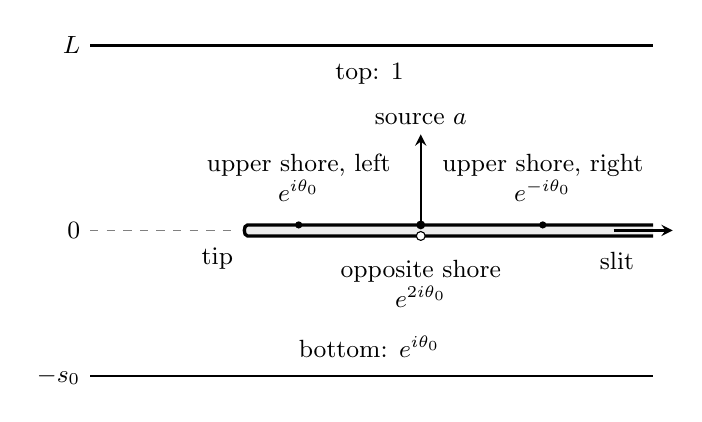
\begin{tikzpicture}[x=1cm,y=1cm,>=stealth,font=\small]
  \draw[thick] (-2,2.35)--(5.15,2.35);
  \draw[thick] (-2,-1.85)--(5.15,-1.85);
  \node[left] at (-2,2.35) {$L$};
  \node[left] at (-2,-1.85) {$-s_0$};
  \draw[dashed,gray] (-2,0)--(-.14,0);
  \node[left] at (-2,0) {$0$};
  \fill[gray!15] (0,.07)--(5.15,.07)--(5.15,-.07)--(0,-.07)
    to[out=180,in=180] (0,.07);
  \draw[very thick] (5.15,.07)--(0,.07)
    to[out=180,in=180] (0,-.07)--(5.15,-.07);
  \draw[->,thick] (4.65,0)--(5.4,0);
  \node[below left] at (-.06,-.1) {tip};
  \node[below right] at (4.35,-.15) {slit};
  \fill (2.2,.07) circle (1.6pt);
  \draw[fill=white] (2.2,-.07) circle (1.6pt);
  \draw[->,thick] (2.2,.12)--(2.2,1.22);
  \node[above] at (2.2,1.22) {source $a$};
  \fill (.65,.07) circle (1.3pt);
  \fill (3.75,.07) circle (1.3pt);
  \node[above,align=center] at (.65,.24)
    {upper shore, left\\$e^{i\theta_0}$};
  \node[above,align=center] at (3.75,.24)
    {upper shore, right\\$e^{-i\theta_0}$};
  \node[below,align=center] at (2.2,-.25)
    {opposite shore\\$e^{2i\theta_0}$};
  \node[below,align=center] at (1.55,2.24) {top: $1$};
  \node[above,align=center] at (1.55,-1.74)
    {bottom: $e^{i\theta_0}$};
\end{tikzpicture}
\caption{The slit domain and the exit phases for an upward-entering
source at distance $a$ from the tip, where $\theta_0=3\pi/8$.
The shores are separated in the drawing to distinguish the two ports
at each cut bond.  A chord to the opposite shore has total tangent turn
$2\pi$; its phase is therefore removed by projection perpendicular to
$e^{2i\theta_0}$.}
\label{R:alt:j:slit-figure}
\end{figure}

\begin{lemma}[Two sources and positive boundary kernels]
\label{R:signed:two-source}
Let $K$ be the positive chord kernel in a convex tessellation polygon.
For adjacent ports $a,b$ in counterclockwise order on a straight boundary
segment and another port $e$, with cyclic order $a<b<e$, let
$K_2(ac,bd)$ denote the mass of mutually vertex-disjoint chord pairs.
Put $r=e^{2i\vartheta}$ and $s=3/8$. Then
\begin{equation}\label{R:alt:j:eq-br4}
K(a,e)-rK(b,e)
 =\sum_{b<d<e}e^{isT(b,d)}K_2(ae,bd)
 -r\sum_{e<c<a}e^{isT(a,c)}K_2(ac,be).
\end{equation}
Consequently same-side kernels decrease as the terminal port moves away
from a fixed source. For every fixed small $\epsilon>0$, the half-plane
kernel confined within distance $H^{1+5\epsilon}$ of its source satisfies
\begin{equation}\label{R:alt:j:eq-br5}
K_{\rm conf}(c,b)\ge H^{-5/4-C\epsilon-o(1)}
\qquad(1\le |b-c|\le H^{1+3\epsilon}).
\end{equation}
\end{lemma}
\begin{proof}
Because $a,b$ lie on the same straight side, $T(a,e)=T(b,e)$; give both
trunks the common phase $e^{isT(a,e)}$ during the following exploration.
Fix a trunk from $a$ to $e$ and grow a turning-weighted stem from $b$,
stopping at its first trunk contact as well as at boundary exits. Compare
this with trunk $b$ to $e$ and stem from $a$. Self-collisions cancel by
the local rule. A contact term is an embedded Y tree with outward arms
in cyclic order $a,b,e$. At its junction, the turn from the $a$ arm onto
the $e$ arm is $+\pi/3$, whereas from the $b$ arm it is $-\pi/3$.
The other turns and all vertex weights agree, so the ratio of the two
contact phases is $e^{is(2\pi/3)}=r$. This also covers immediate contact.
After multiplying the second exploration by $r$, all contact terms cancel.
The remaining disjoint boundary exits have exactly the two cyclic ranges
in \eqref{R:alt:j:eq-br4}; division by the common trunk phase gives that
identity. In strip exhaustions, remote disjoint exits vanish by product
domination and the cap bound.

If $e$ lies beyond $b$ on the same base segment, multiply the identity
by $e^{3i\vartheta}$ and take imaginary parts. The first sum has zero
imaginary part. In the subtracted sum the sine phases are nonnegative,
since $5\vartheta+sT\in[2\vartheta,8\vartheta]$. As
$\sin3\vartheta=\sin5\vartheta>0$, this gives $K(a,e)\le K(b,e)$.
Reversal makes it outward decrease of the terminal from a fixed source;
a tessellation reflection gives the other direction.

To prove the confined lower bound, use a tangent half-hexagonal cap
whose radius is a small constant times $H^{1+5\epsilon}$. Along its base,
the sum of kernels to ports beyond distance $H^{1+4\epsilon}$ is at least
the half-plane tail $A(H^{1+4\epsilon})$ minus the lost mass
$CW_{cH^{1+5\epsilon}}$. By Lemmas~\ref{R:signed:cap}
and~\ref{R:signed:strip-mass}, the second term is negligible and the first
has exponent $-(1+4\epsilon)/4$. There are $O(H^{1+5\epsilon})$ ports
on the cap base. The outward monotonicity just proved bounds the kernel
to every nearer port below by this sum divided by that number. The cap
lies inside the required confinement radius, giving
\eqref{R:alt:j:eq-br5}.
\end{proof}

\begin{lemma}[Top endpoints of two bridges]\label{R:signed:bridge-pair}
Take adjacent bottom ports $a,b$, ordered left to right. Let $b_h(e)$ be
the height-$h$ top kernel from $a$, and put
$D_h(c,d)=K_2(ac,bd)$ for top ports $c<d$, in left-to-right order. Then
\[
 b_h(e)-b_h(e-1)=\sum_{d>e}D_h(e,d)-\sum_{c<e}D_h(c,e),
 \qquad b_h(e)=\sum_{c\le e<d}D_h(c,d),
\]
and
\begin{equation}\label{R:alt:j:eq-br6}
 \sum_{h\ge H}\sum_{c<d}D_h(c,d)\le H^{-1/4+o(1)}.
\end{equation}
\end{lemma}
\begin{proof}
Apply the imaginary-part projection in the preceding proof with $e$ on
the top wall. Bottom exits to the right of $b$ and to the left of $a$
vanish. The top coefficients agree because
$\sin3\vartheta=\sin5\vartheta$, giving the difference identity.
Summing it from the left end of the strip gives the second identity;
the kernel tends to zero at infinity by summability.

For the last bound, join the adjacent bottom ports below the strip by a
three-center arch. Together with the two bridges this gives a downward
half-plane arch from $c$ to $d$. Translate its first port to a fixed
source. The connector has a unique deepest vertex, so the output recovers
the connector, the translation and the original height. Thus the map is
injective over all $h$, with constant weight factor $\rho^3$. Its image
reaches distance at least a constant times $H$, and
\eqref{R:alt:j:finite-boundary} proves the bound.
\end{proof}

We now pass to irreducible pieces, still without any lower length-tail
estimate. Unique decomposition at once-crossed levels gives
\[
 B(z)=\sum_{h\ge0}b_hz^h=\frac1{1-I(z)},\qquad
 I(z)=\sum_{\gamma\in\mathcal I}\rho^{L(\gamma)}z^{H(\gamma)}.
\]
Lemma~\ref{R:signed:strip-mass} gives
$B(e^{-1/H})=H^{3/4+o(1)}$; letting $z\uparrow1$ proves $I(1)=1$.
Thus the critical irreducible weights define the same law $p$ as in
Proposition~\ref{R:renew:factorization}. Write
$\mathsf H,\mathsf X,\mathsf L$ for a block's height, signed horizontal
displacement and length, and let $S$ be its horizontal coordinate range.
Its diameter is at most $C(\mathsf H+S)$.

It will be convenient to name the normalized law of all finite bridges
with weight $\rho^{\mathsf L}z^{\mathsf H}$, including the empty bridge:
call it $\mathbb Q_z$. Under $\mathbb Q_z$, the number of pieces is
geometric with probabilities $(1-I(z))I(z)^k$, $k\ge0$, and, given this
number, their shapes are independent with law
\[
 p_z(d\gamma)=I(z)^{-1}z^{H(\gamma)}p(d\gamma).
\]
This statement concerns different pieces; no independence of the
coordinates within one piece is asserted.

\begin{lemma}[Increment estimates before the lower length bound]
\label{R:signed:increments}
Under $p$,
\begin{equation}\label{R:alt:j:eq-br7}
 \mathbb P_p(\mathsf H>t)=t^{-3/4+o(1)},\qquad
 \mathbb P_p(S>t)\le t^{-3/4+o(1)},\qquad
 \mathbb P_p(\mathsf L>n)\le n^{-9/16+o(1)}.
\end{equation}
In addition, $\mathbb P_p(|\mathsf X|>t)=t^{-3/4+o(1)}$.
\end{lemma}
\begin{proof}
The height deficit is
$\mathbb E_p(1-e^{-\mathsf H/t})=t^{-3/4+o(1)}$, giving the height upper
tail and $\mathbb E[\mathsf H;\mathsf H\le t]\le t^{1/4+o(1)}$.
Evaluate the deficit at $t^{1+\epsilon}$. Heights at most $t$ contribute
only $t^{-3/4-\epsilon+o(1)}$, which is smaller than the deficit
$t^{-3(1+\epsilon)/4+o(1)}$. This proves the lower tail as
$\epsilon\downarrow0$.

Call a block wide if $S>t$, and put
$u=\mathbb E_p[z^{\mathsf H};S>t]$. A bridge containing such a block is
itself wide, so at each height its mass is at most $CW_{ct}$ by the cap
bound. Under $\mathbb Q_z$, the probability of at least one wide block
is exactly
\[
 \frac{B(z)u}{1+B(z)u}.
\]
Take $z=e^{-1/H}$ with $H=t^{1-\epsilon}$. This probability is at most
$CHW_{ct}/B(z)=o(1)$, and hence
$u\le H^{-1/2+o(1)}t^{-1/4+o(1)}$. On $\mathsf H\le H$ the tilt is
bounded below. Add the height-tail bound on the complement and let
$\epsilon\downarrow0$ to obtain the span bound.

The marked-reward identity gives
\[
 \sum_hm_B(h)z^h=B(z)^2\mathbb E_p[\mathsf Lz^{\mathsf H}],
 \qquad \mathbb E_p[\mathsf L e^{-\mathsf H/H}]
       \le H^{7/12+o(1)}.
\]
Splitting according to $\mathsf H>n^{3/4}$ and applying Markov to the
remaining length gives the upper length tail in
\eqref{R:alt:j:eq-br7}.

It remains to prove that the signed displacement has a matching lower
tail. By Lemma~\ref{R:signed:bridge-pair}, bridge weights to any endpoint
windows of size $G$ per row, summed over $R\le h\le2R$, are at most
$C(G+1)R^{-1/4+o(1)}$. For $z=e^{-1/R}$, the whole height bin has
$\mathbb Q_z$-probability $R^{-o(1)}$, whereas the part with
$|\mathsf X_{\rm total}|\le R^{1-\epsilon}$ has probability at most
$R^{-\epsilon+o(1)}$. Thus displacement larger than this threshold has
at least subpower probability.

If every piece had displacement at most $t_*=R^{1-\delta}$, with
$\epsilon\ll\delta$, such a total displacement would be superpolynomially
unlikely. Here are the estimates. Reflection preserves height and
reverses displacement, so the truncated increments
$\mathsf X_{\rm trunc}=\mathsf X\mathbf1_{\{|\mathsf X|\le t_*\}}$
are centered under $p_z$. Their variance is at most $t_*^{5/4+o(1)}$ by the
span tail. The geometric number of pieces exceeds
$R^{3/4+c\delta}$ with superpolynomially small probability for small fixed
$c>0$. For $|v|\le1/t_*$,
\[
 \log\mathbb E_{p_z}e^{v\mathsf X_{\rm trunc}}
   \le C v^2\mathbb E_{p_z}\mathsf X_{\rm trunc}^2.
\]
Both the displacement threshold divided by $t_*$ and its square divided
by the resulting total variance grow as positive powers of $R$.
Exponential Markov therefore gives the claimed negligible probability.
A union bound, using the geometric mean $R^{3/4+o(1)}$, now forces
\[
 \mathbb E_p[z^{\mathsf H};|\mathsf X|>R^{1-\delta}]
       \ge R^{-3/4-o(1)}.
\]
Let $\delta\downarrow0$ and combine with the span upper tail.
\end{proof}

\begin{lemma}[Two ordered renewal arms]\label{R:signed:two-arms}
Start independent infinite $p$-sequences at adjacent bottom ports,
designated left and right. Let $P_m$ be the following event:
\begin{itemize}
\item the paths formed by the first $m$ pieces of the two arms are disjoint;
\item for each pair of positive renewal indices at most $m$, if their
heights are $n\le p$, every crossing of line $n$ by the height-$p$ prefix
lies strictly on its designated side of the other arm's endpoint at $n$.
When $n=p$, this means that the two endpoints are ordered.
\end{itemize}
Then
\begin{equation}\label{R:alt:j:eq-br8}
 p_m:=\mathbb P(P_m)\le m^{-1+o(1)}.
\end{equation}
\end{lemma}
\begin{proof}
Fix a small $\delta>0$, and set
\[
 L=\lceil m^{4/3+\delta}\rceil,\qquad G=m^{4/3-\delta}.
\]
We first show that, outside a superpolynomially small event, on each arm
at most $m/4$ renewal endpoints lie within horizontal distance $G$ of the
pertinent extreme crossing of the other full infinite path at that height.
The pertinent crossing is the leftmost on the right arm or the rightmost
on the left arm; it exists because the path reaches every height.

Condition on the other path. Divide the renewal indices into residue
classes modulo $m_0=\lfloor m^{1-c\delta}\rfloor$, with a small fixed
$c>0$. Successive sampled endpoints in one class are separated by a
fresh chunk of $m_0$ independent pieces. By the displacement lower tail
in Lemma~\ref{R:signed:increments}, such a chunk contains a positive
power of $m$ increments with magnitude greater than $2G$, except with
probability tending to zero. Conditional on all chunk heights and
absolute displacements, their nonzero signs are independent fair signs.
The target crossing position depends on the heights and the other path,
but not these signs.

If there are $k$ increments of magnitude greater than $2G$, their signed
sum lands in an interval of width $2G$ with probability at most
$C/\sqrt{k}$. Indeed, after fixing the other signs, the subsets of positive
large signs that yield a sum in that interval form an antichain: adding
one such sign changes the sum by more than $4G$. Counting maximal chains
bounds its size by the middle binomial coefficient. Thus the conditional
window probability at each sampled endpoint tends uniformly to zero.
Successive conditioning makes a positive fraction of hits in any residue
class exponentially unlikely in $m/m_0$. Union over the classes proves
the assertion about at most $m/4$ close endpoints; the initial incomplete
chunk costs at most $m_0=o(m)$ indices.

Suppose now that $P_m$ holds, both total heights are at most $L$, and the
exception above does not occur. There are at least $cm^2$ pairs of renewal
indices for which the two prefixes are disjoint and their gap at the
shorter height exceeds $G$. Crossings there by the longer prefix equal
those by its full path: later pieces lie strictly above its endpoint.
We claim that the expected number of all such height-bounded pairs is
\begin{equation}\label{R:signed:gap-pairs}
 O(1)+O(L^{7/4+o(1)}/G).
\end{equation}
Summing over renewal prefixes gives ordinary bridge weights. Equal-height
pairs have bounded total mass by \eqref{R:alt:j:eq-br6}. For unequal
heights, fix their difference $s_0=p-n>0$ and which arm is shorter.
Join their adjacent bottom starts by the three-center connector used in
Lemma~\ref{R:signed:bridge-pair}.

At row $n$, choose a tessellation vertex between the shorter endpoint and
the extreme crossing of the longer prefix. The gap gives at least $cG$
choices. From that tip cut the horizontal ray pointing away from the
longer path's crossings, through the shorter endpoint. The joined path
avoids the slit: the shorter bridge is strict below its endpoint, and
all crossings of the longer bridge at this row are on the other side.
It starts at the slit shore, goes toward the connector, and terminates
on the line of height $p$.

The map is illustrated in Figure~\ref{R:alt:j:pair-slit-figure}.
Send the tip $(t,n)$ to the origin. If the shorter endpoint is on the
right, use $(x',y')=(x-t,n-y)$; if it is on the left, use
$(x',y')=(t-x,n-y)$. These tessellation symmetries make the slit rightward
and the initial shore upper. The endpoint is on $y'=-s_0$, while the
unique highest vertex, on the connector, has $y'=n+2/3$. The path is
therefore counted by the slit estimate with upper wall $L+1$. Conversely,
its unique highest vertex recovers $n$, the connector and the original
translation, and hence both bridges and the chosen tip. For the fixed
assignment this map is injective, with a fixed weight factor. Summing
\eqref{R:alt:j:eq-br3} over the slit sources and dividing by the $cG$
tip choices bounds the pair mass, already summed over $n\le L$, by
$CL^{3/4+o(1)}/G$. Sum over the at most $L$ height differences to obtain
\eqref{R:signed:gap-pairs}.

Division by $cm^2$ now bounds $p_m$ in the restricted height range by
$m^{-1+C\delta+o(1)}$. To remove that restriction, set
$t=m^{4/3+\delta/2}$. Exponential Markov at $1/t$, together with
$\mathbb E[\mathsf H;\mathsf H\le t]\le t^{1/4+o(1)}$, shows that a
sum of $m$ heights exceeding $L$ with no increment above $t$ has
superpolynomially small probability. A height above $t$ at index $j$
on either arm is independent of $P_{j-1}$. Thus
\[
 p_m\le Cm^{-1+C'\delta+o(1)}
       +Cm^{-1-c'\delta}\sum_{j<m}p_j,
 \qquad p_0=1,
\]
for some $c'>0$. Induction gives $p_m=O_\eta(m^{-1+\eta})$ whenever
$\eta>C'\delta$: under this bound the second term is
$O(m^{-1+\eta-c'\delta})$. Choose $\delta$ arbitrarily small to obtain
\eqref{R:alt:j:eq-br8}.
\end{proof}

\begin{figure}[ht]
\centering
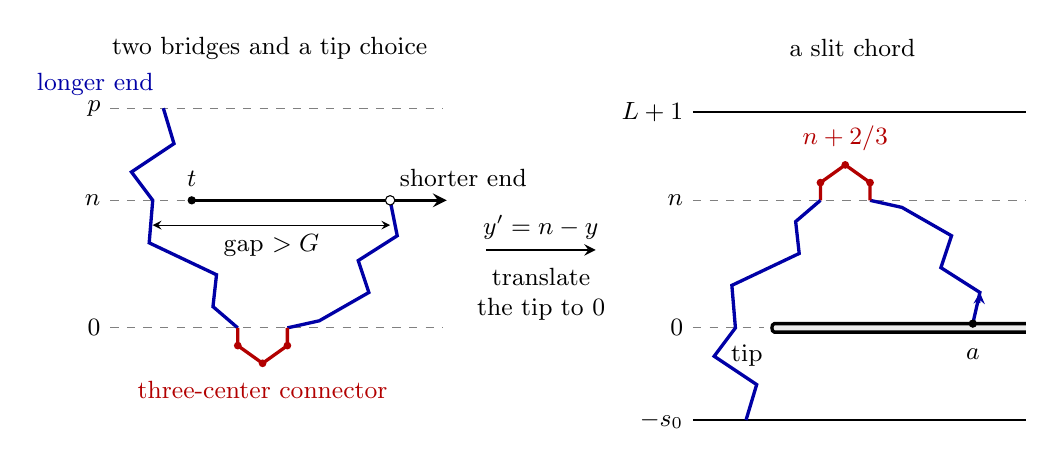
\begin{tikzpicture}[x=.9cm,y=.9cm,>=stealth,font=\small]
  \begin{scope}
    \node[align=center] at (1.1,3.95) {two bridges and a tip choice};
    \foreach \y/\lab in {0/{0},1.8/{n},3.1/{p}}
      {\draw[dashed,gray] (-1.15,\y)--(3.55,\y);
       \node[left] at (-1.15,\y) {$\lab$};}
    \draw[very thick,blue!65!black] (.65,0)--(.3,.3)--(.35,.75)
      --(-.6,1.2)--(-.55,1.8)--(-.85,2.2)--(-.25,2.6)--(-.4,3.1);
    \draw[very thick,blue!65!black] (1.35,0)--(1.8,.1)--(2.5,.5)
      --(2.35,.95)--(2.9,1.3)--(2.8,1.8);
    \draw[very thick,red!70!black] (.65,0)--(.65,-.25)
      --(1,-.5)--(1.35,-.25)--(1.35,0);
    \foreach \x/\y in {.65/-.25,1/-.5,1.35/-.25}
      {\fill[red!70!black] (\x,\y) circle (1.4pt);}
    \draw[very thick,->] (0,1.8)--(3.6,1.8);
    \fill (0,1.8) circle (1.5pt);
    \draw[fill=white] (2.8,1.8) circle (1.7pt);
    \node[above] at (0,1.86) {$t$};
    \node[above right] at (2.8,1.86) {shorter end};
    \node[below,red!70!black] at (1,-.62) {three-center connector};
    \draw[<->] (-.55,1.45)--(2.8,1.45)
      node[midway,below] {gap $>G$};
    \node[above left,blue!65!black] at (-.4,3.15) {longer end};
  \end{scope}
  \draw[->,thick] (4.15,1.1)--(5.7,1.1)
    node[midway,above,align=center] {$y'=n-y$};
  \node[below,align=center] at (4.93,.98) {translate\\the tip to $0$};
  \begin{scope}[xshift=7.4cm]
    \node[align=center] at (1.1,3.95) {a slit chord};
    \draw[thick] (-1.15,3.05)--(3.55,3.05);
    \draw[thick] (-1.15,-1.3)--(3.55,-1.3);
    \node[left] at (-1.15,3.05) {$L+1$};
    \node[left] at (-1.15,-1.3) {$-s_0$};
    \draw[dashed,gray] (-1.15,1.8)--(3.55,1.8);
    \node[left] at (-1.15,1.8) {$n$};
    \draw[dashed,gray] (-1.15,0)--(-.14,0);
    \node[left] at (-1.15,0) {$0$};
    \fill[gray!15] (0,.06)--(3.55,.06)--(3.55,-.06)--(0,-.06)
      to[out=180,in=180] (0,.06);
    \draw[very thick] (3.55,.06)--(0,.06)
      to[out=180,in=180] (0,-.06)--(3.55,-.06);
    \draw[very thick,blue!65!black] (2.8,.06)--(2.9,.5)--(2.35,.85)
      --(2.5,1.3)--(1.8,1.7)--(1.35,1.8);
    \draw[very thick,red!70!black] (1.35,1.8)--(1.35,2.05)
      --(1,2.3)--(.65,2.05)--(.65,1.8);
    \foreach \x/\y in {.65/2.05,1/2.3,1.35/2.05}
      {\fill[red!70!black] (\x,\y) circle (1.4pt);}
    \draw[very thick,blue!65!black] (.65,1.8)--(.3,1.5)--(.35,1.05)
      --(-.6,.6)--(-.55,0)--(-.85,-.4)--(-.25,-.8)--(-.4,-1.3);
    \fill (2.8,.06) circle (1.5pt);
    \draw[->,blue!65!black,thick] (2.89,.35)--(2.9,.5);
    \node[below] at (2.8,-.16) {$a$};
    \node[above,red!70!black] at (1,2.36) {$n+2/3$};
    \node[below left] at (-.03,-.1) {tip};
  \end{scope}
\end{tikzpicture}
\caption{The pair-to-slit map when the shorter arm is on the right.
Choose a tessellation vertex $t$ in the gap at height $n$, and direct
the slit through the shorter endpoint.  After reflection across that
level and translation of the tip, the shorter endpoint is an upper-shore
source and the longer endpoint is on the bottom line
$-s_0=-(p-n)$.  The unique maximum, at height $n+2/3$, identifies the
connector and recovers $n$.  If the shorter arm is on the left, a
half-turn about $t$ gives the same orientation.  Heights and paths are
schematic, and the two slit shores are separated only for display.}
\label{R:alt:j:pair-slit-figure}
\end{figure}

\subsection{Folding uniformly around a prescribed irreducible}

Fold a half-plane arch of exact maximum layer $k$ at its leftmost highest
down triangle. Split there, ending the first arm and starting the second
at the port above that triangle on line $k$, and reflect the second arm
across that line. The result is a height-$2k$ bridge, with a renewal at
$k$. The highest triangle was counted twice, so the folded weight is
$\rho$ times the arch weight. Unfolding at that middle renewal recovers
the arch, making this map injective.

Call a segment of an ordinary bridge \emph{valid} if its endpoints and
middle are renewal positions, at heights $c-k,c,c+k$, and it is the image
of this fold up to translation. Endpoints of the whole bridge are allowed.
Fix positive constants $c_1,C_1,C_2$ and a small $\epsilon>0$. Let $K$ count
valid segments whose half-height satisfies
\[
 c_1H\le k\le H^{1+C_1\epsilon}.
\]
The essential bound is uniform in the shape and length of a single fixed
irreducible; this is what will permit marking a long block later.

\begin{lemma}[Folding with a fixed irreducible]\label{R:signed:folding}
Fix an irreducible $\xi$ of height $d$. Place independent
$\mathbb Q_z$ bridges below and above it, translating $\xi$ to the joining
port, where $z=e^{-1/T}$ and $T=H^{1+C_2\epsilon}$. Write $\mathbb E^*_\xi$
for this law. Uniformly in $\xi$,
\begin{equation}\label{R:alt:j:eq-br9}
 \mathbb E^*_\xi K\le H^{1/2+O(\epsilon)+o(1)}.
\end{equation}
\end{lemma}
\begin{proof}
First count valid segments wholly outside $\xi$. Marking such a segment
in either exterior bridge gives two ordinary bridge factors and the folded
arch factor. One bridge normalization cancels, so this contribution is at
most
\[
 2\rho B(z)\sum_{k\text{ in range}}a_kz^{2k}
 \le 2\rho B(z)\sum_{k\ge c_1H}a_k
 \le H^{1/2+O(\epsilon)+o(1)}.
\]
The last inequality uses $B(z)=T^{3/4+o(1)}$ and the arch radius tail.

Every other valid segment contains the whole defect. Its middle renewal
cannot lie strictly inside an irreducible. Suppose first that this renewal
is $l\ge0$ levels below the start of $\xi$; the other case follows by
reversal and height reflection, which preserve the leftmost rule and
replace $\xi$ by a fixed transformed defect if necessary.

Here is the normalization cancellation for these segments. Cut at their
two endpoint renewals. The ordinary pieces outside the segment are free
and contribute $B(z)^2$, canceling the two exterior normalizations. Thus
for this orientation their contribution to $\mathbb E^*_\xi K$ is the sum,
over valid internal segments containing the fixed defect, of
\[
 \rho^{L(\text{segment})-L(\xi)}z^{2k-d}.
\]
There is no weight for the prescribed defect in this expression and no
sum over an independently chosen joining port. Unfolding the segment
at its middle gives two arms of height $k$: one ordinary bridge, and
one ordinary bridge of height $l$, followed by $\xi$, followed by an
ordinary bridge of height $k-l-d$. The pieces have total ordinary height
$2k-d$, as in the displayed weight. Reversed or reflected ordinary pieces
can be rooted at their first port by translation. Figure~\ref{R:alt:j:fold-figure}
shows these heights.

\begin{figure}[ht]
\centering
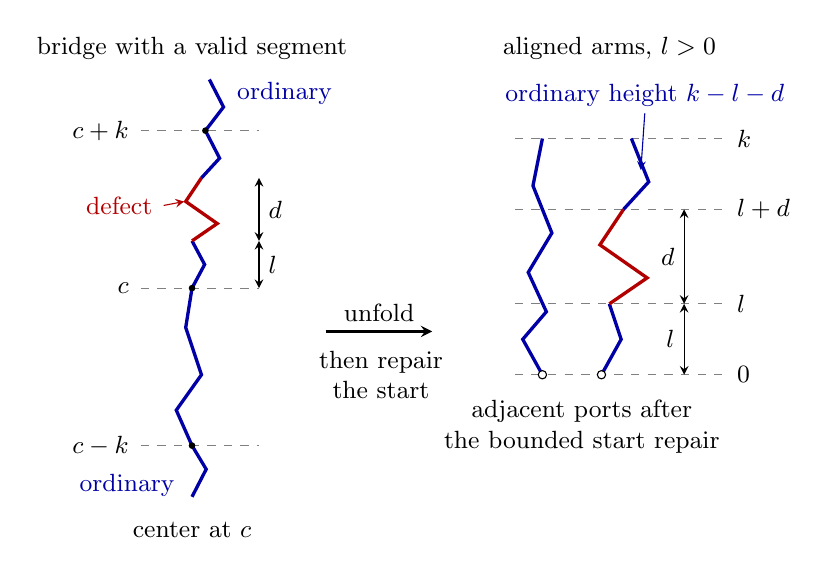
\begin{tikzpicture}[x=1cm,y=1cm,>=stealth,font=\small]
\begin{scope}[xshift=1.4cm]
\node[align=center]at(0,3.05){bridge with a valid segment};
\foreach \y/\lab in {-2/{c-k},0/{c},2/{c+k}}
 {\draw[dashed,gray](-.65,\y)--(.85,\y);
  \node[left]at(-.68,\y){$\lab$};}
\draw[very thick,blue!65!black] (0,-2.65)--(.18,-2.3)--(0,-2)
 --(-.2,-1.55)--(.12,-1.1)--(-.08,-.5)--(0,0)
 --(.16,.3)--(0,.6);
\draw[very thick,red!70!black] (0,.6)--(.32,.82)--(-.08,1.1)--(.12,1.4);
\draw[very thick,blue!65!black] (.12,1.4)--(.35,1.65)--(.17,2)
 --(.4,2.3)--(.22,2.65);
\foreach \x/\y in {0/-2,0/0,.17/2}{\fill(\x,\y)circle(1.2pt);}
\node[left,blue!65!black]at(-.1,-2.5){ordinary};
\node[right,blue!65!black]at(.45,2.48){ordinary};
\node[left,red!70!black]at(-.38,1.05){defect};
\draw[red!70!black,thin,->](-.36,1.05)--(-.10,1.10);
\draw[<->](.85,0)--(.85,.6)node[midway,right]{$l$};
\draw[<->](.85,.6)--(.85,1.4)node[midway,right]{$d$};
\node[below,align=center]at(0,-2.85){center at $c$};
\end{scope}
\draw[->,thick](3.1,-.55)--(4.45,-.55)
 node[midway,above,align=center]{unfold};
\node[align=center]at(3.8,-1.1){then repair\\the start};
\begin{scope}[xshift=5.5cm,yshift=-1.1cm]
\node[align=center]at(1.2,4.15){aligned arms, $l>0$};
\foreach \y/\lab in {0/{0},.9/{l},2.1/{l+d},3/{k}}
 {\draw[dashed,gray](.0,\y)--(2.65,\y);
  \node[right]at(2.7,\y){$\lab$};}
\draw[very thick,blue!65!black] (.35,0)--(.1,.45)--(.4,.8)
 --(.17,1.3)--(.47,1.8)--(.23,2.4)--(.35,3);
\draw[very thick,blue!65!black] (1.1,0)--(1.35,.45)--(1.2,.9);
\draw[very thick,red!70!black] (1.2,.9)--(1.68,1.23)--(1.08,1.65)--(1.38,2.1);
\draw[very thick,blue!65!black] (1.38,2.1)--(1.7,2.45)--(1.48,3);
\foreach \x in {.35,1.1}{\draw[fill=white](\x,0)circle(1.5pt);}
\draw[<->](2.15,0)--(2.15,.9)node[midway,left]{$l$};
\draw[<->](2.15,.9)--(2.15,2.1)node[midway,left]{$d$};
\node[align=left,blue!65!black]at(1.65,3.55){ordinary height $k-l-d$};
\draw[blue!65!black,thin,->](1.65,3.32)--(1.6,2.6);
\node[below,align=center]at(.85,-.2){adjacent ports after\\the bounded start repair};
\end{scope}
\end{tikzpicture}
\caption{Unfolding a valid segment containing a fixed irreducible defect, in the case $l>0$ and $l+d\le k$. The ordinary pieces outside the segment are omitted on the right. The red defect is unchanged; the bounded repair acts at the common start and produces the adjacent disjoint starts shown on the right. Heights are schematic and individual lattice edges are suppressed. The two exterior factors $B(z)$ cancel the normalizations by the cutting argument in the text, independently of this drawing.}
\label{R:alt:j:fold-figure}
\end{figure}

If $l=0$, dropping avoidance already bounds the aligned arm sum by
$T^{1/2+o(1)}$, using the squared-sum estimate below. Suppose $l>0$.
The unfolded arms initially meet only at their common port and first
down triangle, and take its distinct slant branches. They must be turned
into disjoint arms from adjacent ports before Lemma~\ref{R:signed:two-arms}
can be used.

Orient the unfolding downward and put its common port at $P=(0,0)$.
Write $h_0=\sqrt3/2$. The first down center is $D=(0,-h_0/3)$;
the left branch next visits $U=(-1/2,-2h_0/3)$. Replace the initial
portion $P,D,U$ of this branch by
\[
 P_-=(-1,0),\qquad D_-=(-1,-h_0/3),\qquad U.
\]
These are actual neighboring ports and centers, as shown in
Figure~\ref{R:alt:j:start-repair}. The center $D_-$ is unused by both
arms, because $D$ was chosen as the leftmost visited highest down
triangle of the arch. From $U$ the next edge cannot return to $D$ or
visit $D_-$, so it continues downward. The replacement therefore preserves
self-avoidance and makes the two arms disjoint. It substitutes one vertex
for one vertex, preserving each length and weight. All changed edges lie
at depths less than one; every positive integral-depth crossing and its
order is unchanged. Since $l\ge1$, the fixed defect is untouched.

The inverse restores the left initial portion using the unchanged right
port and first center. Keep the finitely many choices of arm and symmetry
as separate assignments. After reanchoring the adjacent starts at fixed
ports, the unchanged far endpoint and the original anchor determine the
translation back. This gives bounded inverse multiplicity with no
height-dependent factor.

\begin{figure}[ht]
\centering
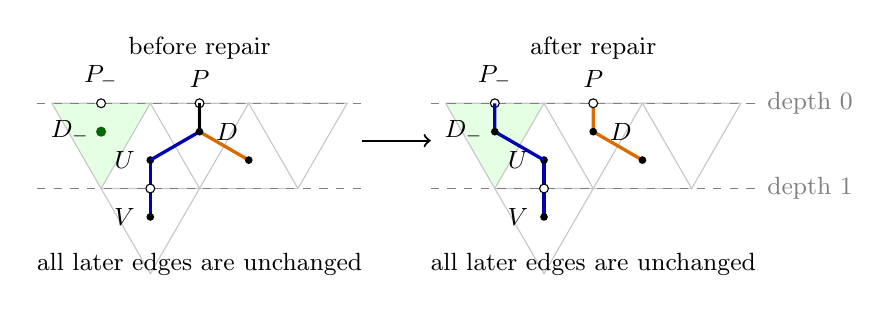
\begin{tikzpicture}[x=1.25cm,y=1.25cm,font=\small,
  lattice/.style={gray!45,thin},
  leftarm/.style={blue!70!black,very thick},
  rightarm/.style={orange!85!black,very thick}]
\pgfmathsetmacro{\hh}{sqrt(3)/2}
\foreach \shift/\panel in {0/{before repair},5/{after repair}} {
  \begin{scope}[xshift=\shift cm]
    \fill[green!10] (-1.5,0)--(-.5,0)--(-1,-\hh)--cycle;
    \foreach \xx in {-1,0,1} {
      \draw[lattice] ({\xx-.5},0)--({\xx+.5},0)
        --(\xx,-\hh)--cycle;
    }
    \draw[lattice] (-1,-\hh)--(1,-\hh);
    \draw[lattice] (-1,-\hh)--(0,-\hh)
      --(-.5,{-2*\hh})--cycle;
    \draw[gray,dashed] (-1.65,0)--(1.65,0);
    \draw[gray,dashed] (-1.65,-\hh)--(1.65,-\hh);
    \node[above] at (0,.35) {\panel};
    \node[above] at (0,.06) {$P$};
    \node[above] at (-1,.06) {$P_-$};
    \node[left] at (-1.02,{-\hh/3}) {$D_-$};
    \node[right] at (.07,{-\hh/3}) {$D$};
    \node[left] at (-.56,{-2*\hh/3}) {$U$};
    \node[left] at (-.56,{-4*\hh/3}) {$V$};
    \draw[rightarm] (0,0)--(0,{-\hh/3})
      --(.5,{-2*\hh/3});
    \draw[leftarm] (-.5,{-2*\hh/3})--(-.5,{-4*\hh/3});
    \fill (.5,{-2*\hh/3}) circle (1.4pt);
    \fill (-.5,{-2*\hh/3}) circle (1.4pt);
    \fill (-.5,{-4*\hh/3}) circle (1.4pt);
    \draw[fill=white] (0,0) circle (1.6pt);
    \draw[fill=white] (-1,0) circle (1.6pt);
    \draw[fill=white] (-.5,-\hh) circle (1.6pt);
    \node[below,align=center] at (0,{-1.65*\hh})
      {all later edges are unchanged};
  \end{scope}
}
\begin{scope}
  \draw[leftarm] (0,{-\hh/3})--(-.5,{-2*\hh/3});
  \draw[very thick] (0,0)--(0,{-\hh/3});
  \fill (0,{-\hh/3}) circle (1.4pt);
  \draw[fill=white,green!40!black] (-1,{-\hh/3}) circle (1.6pt);
\end{scope}
\begin{scope}[xshift=5cm]
  \draw[leftarm] (-1,0)--(-1,{-\hh/3})--(-.5,{-2*\hh/3});
  \fill (-1,{-\hh/3}) circle (1.4pt);
  \fill (0,{-\hh/3}) circle (1.4pt);
  \node[right,gray] at (1.67,0) {depth $0$};
  \node[right,gray] at (1.67,-\hh) {depth $1$};
\end{scope}
\draw[->,thick] (1.65,-.38)--(2.35,-.38);
\end{tikzpicture}
\caption{The exact local start repair in the downward unfolding
orientation. Put $h_0=\sqrt3/2$. The relevant centers are
$D=(0,-h_0/3)$, $D_-=(-1,-h_0/3)$,
$U=(-1/2,-2h_0/3)$ and $V=(-1/2,-4h_0/3)$;
the ports are $P=(0,0)$ and $P_-=(-1,0)$.
The two arms originally share $P$ and $D$; the green triangle contains
$D_-$, which is unused before the repair.
Replace $P,D,U$ on the left branch by $P_-,D_-,U$.
The picture takes $k\ge2$, as holds in the defect case $l>0$;
for a height-one arm the displayed continuation stops at the
port $(-1/2,-h_0)$ before $V$.
Only the displayed local path is specified; no continuation choice
is asserted beyond the displayed endpoints.}
\label{R:alt:j:start-repair}
\end{figure}

A simple strip crosscut meeting a level just once separates its two
horizontal rays. Consequently, whenever either repaired full bridge
renews, all crossings of the other at that level lie on the prescribed
side of its endpoint; the endpoints on the two exterior lines are ordered
as well. This supplies the ordering condition used next.

Let the ordinary prefix on the defect arm contain $m$ blocks and end at
height $l$. Expose the other arm through its first renewal at height
$p\ge l$. Sum the remaining ordinary portions, discarding their avoidance
constraints. Cauchy--Schwarz applied to the shifted sequence
$(b_jz^j)_{j\ge0}$ bounds the alignment cost uniformly in $l,p,d$ by
\[
 \sum_{k\ge\max(p,l+d)} b_{k-p}b_{k-l-d}
          z^{(k-p)+(k-l-d)}
 \le\sum_{j\ge0}b_j^2z^{2j}\le T^{1/2+o(1)}.
\]

After this summation the exposed portions can be counted as independent
$p$-sequences: the first $m$ blocks on the defect arm and the other arm
stopped at its first renewal at or above $l$. Their necessary disjointness
and ordering conditions imply $P_m$. If at least $m$ blocks of the other
arm have been exposed, restrict to its first $m$. If fewer have been
exposed, extend that arm by ordinary blocks: they stay beyond $p\ge l$
and neither meet the defect arm's ordinary prefix nor alter crossings at
its renewal levels. Thus every such extension has the required conditions
for the first $m$ blocks of both arms. This explains why a probability
bound for two equally indexed prefixes applies to the unequal stopping
rule.

Retain the tilt $z^l$ on the $m$ ordinary blocks of the defect arm, and
drop the other exposed tilt factors. For
$m\le T^{3/4+\delta'}$, Lemma~\ref{R:signed:two-arms} bounds the sum of
exposed-prefix weights by
\[
 \sum_{m\le T^{3/4+\delta'}}p_m=T^{o(1)}.
\]
For larger $m$, discard ordering instead and use $I(z)^m$; since
$1-I(z)=T^{-3/4+o(1)}$, that tail is negligible for each fixed
$\delta'>0$. Multiplying by the alignment bound proves
\eqref{R:alt:j:eq-br9} for segments containing the defect, and hence for
all valid segments.
\end{proof}

\subsection{Recoverable cuts and the second moment of finite chords}

We have obtained the folding estimate needed to transfer a long finite
path to a long irreducible. We now prove that there are enough long finite
paths. The remaining moment bound comes from closing a chord into an
unrooted polygon. To keep its inverse multiplicity small, we must first
control how many levels can serve as recoverable cuts of that polygon.

\begin{lemma}[The number of recoverable cuts]\label{R:signed:cut-counts}
For every fixed $\epsilon>0$, polygons of diameter at most $Q$, counted
once per translation class, have the following properties outside a set
whose total critical weight is smaller than every inverse power of $Q$:
\begin{itemize}
\item in each tessellation direction, at most $Q^{1/2+\epsilon}$ levels
are crossed exactly twice;
\item for each such two-crossing level and either polygon arc that it
cuts off, at most $Q^{3/4+\epsilon}$ levels in either other direction
are crossed exactly once by that arc.
\end{itemize}
The second bound also holds for the single crossings of a fixed-source
half-plane arch of diameter at most $Q$ in a direction nonparallel to its
boundary, with the same exceptional-mass conclusion. These conclusions
remain true after multiplication of the exceptional weights by any fixed
polynomial in the lengths.
\end{lemma}
\begin{proof}
If a polygon has many exact-two levels in one direction, cut at their two
extremes. There is an outer arch on each side, and between the extremes
there are two through-bridges: the other pairing would disconnect the
single cycle. Every intermediate exact-two level is a common renewal of
these bridges. Fixing the extreme levels and ports modulo translation
costs a polynomial in $Q$. The outer arches have bounded mass. Drop
avoidance between the through-bridges and count their prefixes as two
independent $p$-sequences.

Let $N_Q$ count their common renewal heights up to $CQ$. For every fixed
positive integer $r$, the renewal property gives
\[
 \mathbb E\binom{N_Q}{r}
 \le\left(\sum_{j\le CQ}b_j^2\right)^r
 \le Q^{r/2+o(1)}.
\]
One obtains the first inequality by listing the $r$ common hits in order
and summing the independent height increments between consecutive hits.
Therefore
\[
 \mathbb P\{N_Q\ge Q^{1/2+\epsilon}\}
 \le
 \frac{Q^{r/2+o(1)}}{\binom{\lfloor Q^{1/2+\epsilon}\rfloor}{r}}
 =Q^{-r\epsilon+o(1)}.
\]
Taking $r$ as large as needed absorbs the polynomial specification cost
and any fixed polynomial length factor.

For the second assertion, fix the original cut level and one arc. Its
endpoints are ports on that line, so neither lies on a tessellation line
in a different direction. Take the first and last, in level order, among
the alleged many exact-one crossings in the second direction. The portion
between them is a strict through-bridge and all intermediate exact-one
levels are its renewals. For a single sequence the same argument uses
\[
 \sum_{j\le CQ}b_j\le Q^{3/4+o(1)}
\]
in place of the squared sum, and the threshold is $Q^{3/4+\epsilon}$.
The end portions lie between the cutting-line constraint and the
corresponding extreme-level constraint, so they are boundary chords in
convex wedges and have bounded mass. The other polygon arc is a
bounded-mass half-plane arch. Fixing their cut ports and levels costs
only a polynomial. For a fixed-source arch use its base line in place
of the polygon's first cutting line; the same decomposition applies.
Finally every path of diameter at most $Q$ has $O(Q^2)$ vertices, so fixed
polynomial length factors are harmless. Crossings throughout are at bond
midpoints.
\end{proof}

\begin{lemma}[Chord second moment]\label{R:signed:chord-square}
For the middle-visiting chord ensemble summed over $H\le R\le2H$,
\begin{equation}\label{R:alt:j:eq-cl1}
 \sum_{R,\ \mathrm{chords}}\rho^{\mathsf L}\mathsf L^2
       \le H^{53/12+o(1)}.
\end{equation}
\end{lemma}
\begin{proof}
Use the regular hexagons $D_R$ in the finite input, summed over integers $H\le R\le2H$. Consider ordered chords that visit the middle region (some center within $R/10$ of the middle). Their mass is at most $H^{7/4+o(1)}$ by the boundary estimate. Their length sum is at least $H^{37/12-o(1)}$ by the imported bulk-visit lower bound (at least $R^{2+1/12-o(1)}$ per hexagon). Close chords with additional paths, using a small $\epsilon>0$ and polygons of diameter $\le Q=H^{1+6\epsilon}$. All pieces joined at ports below have disjoint center sets and weights just multiply. Fix endpoint side choices, finitely many possibilities.

\begin{itemize}
\item If both endpoints are on the same side, join them by an independent arch in its exterior half-plane. By \eqref{R:alt:j:eq-br5} the confinement toll (total available factor) is at least $H^{-5/4-C\epsilon-o(1)}$. That side level has exactly two crossings in the polygon. For a given nonexceptional polygon up to translation and fixed $R$, there are at most $Q^{1/2+\epsilon}$ choices for the cut level, and $O(H)$ more for translation along it (place a port on the side); the pieces can then be read from the polygon up to bounded choices.

\item If the sides are nonparallel, denote their lines by $v=0$ (source side) and $u=0$ (destination side), signed oblique level coordinates chosen so the interior lies at $u<0,v>0$. These tessellation lines meet at a lattice vertex at distances $O(H)$ from the two endpoints $a,b$. Join $a$ into the exterior wedge $u<0,v<0$ to an exit port $c$ on $u=0$. Both possible wedge angles are covered by the confined other-ray bound after \eqref{R:alt:j:eq-br1}; use radii $\le H^{1+\epsilon}$. Then join $c$ to $b$ in the half-plane $u>0$. By \eqref{R:alt:j:eq-br5} the joint toll is at least $H^{-3/2-C\epsilon-o(1)}$. Now $u=0$ has exactly two crossings, and in the arc in $u<0$ the level $v=0$ has exactly one. Thus the translation choices at each $R$ cost at most $Q^{1/2+\epsilon}Q^{3/4+\epsilon}$ for nonexceptional polygons; the two level placements determine the translation, and the three pieces are recovered from the cuts.

\item For opposite parallel sides orient the strip vertically in height, the chord a bridge from $a$ to $b$ of height $h=2R$. Use an independent second height-$h$ bridge, started to the right of $a$ at an integer gap in $[H^{1+2\epsilon},2H^{1+2\epsilon}]$, confined within radius $H^{1+\epsilon}$ of its start. This has mass $h^{-1/4+o(1)}$ by \eqref{R:alt:j:eq-br1} and the cap comparison, and is separate from the chord. Join the pairs of ends by arches below and above the strip using \eqref{R:alt:j:eq-br5}. Including the gap choices, the toll is at least $H^{-7/4-C\epsilon-o(1)}$. Across all $R$, the two cut levels both have exact-two crossings, and determine $h$, hence $R$; thus multiplicity for a nonexceptional polygon is at most $C Q^{1+2\epsilon}H$, including translation along the source side. The original pieces and the gap are then read off up to bounded choices.

\end{itemize}
In each case the number of inverse specifications even in the exceptional set is only polynomial (port assignments and translations in bounded ranges). Thus by \eqref{R:alt:j:polygon-input} and the observations above, counting polygon lengths squared (which majorize the chord lengths squared) costs $Q^{2/3+o(1)}$ times the stated multiplicities, plus negligible errors. To display the losses, suppress the already specified $O(\epsilon)+o(1)$ corrections. The leading exponents from the inverse toll and the inverse count (including the $R$ sum) are
\[
\begin{aligned}
\text{same side:}&\quad \tfrac54+\tfrac52=\tfrac{15}4,\\
\text{nonparallel sides:}&\quad \tfrac32+\tfrac94=\tfrac{15}4,\\
\text{opposite sides:}&\quad \tfrac74+2=\tfrac{15}4.
\end{aligned}
\]
In the first two cases one sums over $R$; in the opposite-side case the two recovered cut levels already determine $R$. Including the polygon second-moment exponent gives $15/4+2/3=53/12$. Let $\epsilon\downarrow0$ to obtain \eqref{R:alt:j:eq-cl1}.

\end{proof}

\begin{corollary}[Mass of long middle-visiting chords]\label{R:signed:long-chords}
For every small fixed $\delta>0$, the middle-visiting chords with
$\mathsf L\ge H^{4/3-\delta}$, summed over $H\le R\le2H$, have critical
mass at least $H^{7/4-o(1)}$.
\end{corollary}
\begin{proof}
The shorter chords carry first-length mass at most
$H^{4/3-\delta}M_0(H)\le H^{37/12-\delta+o(1)}$, negligible relative to
$M_1(H)\ge H^{37/12-o(1)}$. Thus the long chords retain first-length mass
$H^{37/12-o(1)}$. Cauchy--Schwarz and
Lemma~\ref{R:signed:chord-square} give their mass at least
\[
 \frac{H^{2(37/12)-o(1)}}{H^{53/12+o(1)}}=H^{7/4-o(1)}.
\]
\end{proof}

\subsection{The lower length tail and its changes of law}

We can now combine the finite moment estimate with the uniform folding
bound. The bridge law $\mathbb Q_z$ introduced above is useful here because
marking one large irreducible leaves two independent ordinary bridges.

\begin{proof}[Proof of Theorem~\ref{R:alt:j:theorem}]
Fix a small $\eta>0$, choose $0<\epsilon\ll\delta\ll\eta$, and put
\[
 n=H^{4/3-\eta},\qquad T=H^{1+3\epsilon},\qquad z=e^{-1/T},
 \qquad u=\mathbb E_p[z^{\mathsf H};\mathsf L\ge n].
\]
Call the chords supplied by Corollary~\ref{R:signed:long-chords}
\emph{long}; their lengths are at least $H^{4/3-\delta}$.

\emph{From long chords to bridges or arches.}
There are finitely many assignments of endpoint sides. At least one
assignment carries mass $H^{7/4-o(1)}$, though the assignment may vary
with $H$. Its conversion is as follows.
\begin{itemize}
\item For opposite sides, the chord is already a bridge of height $h=2R$.
There are $O(H)$ possible source placements at each $R$, and $h$
determines $R$. Translating to a fixed source gives long bridge mass,
summed over $2H\le h\le4H$, at least $H^{3/4-o(1)}$.

\item For the same side, regard the chord as an arch in its inward
half-plane. Visiting the middle forces its maximum layer between $c_0H$
and $CH$. There are $O(H^2)$ choices of $R$ and source placement, so after
translation its long arch mass is at least $H^{-1/4-o(1)}$.

\item For nonparallel sides, use the oblique coordinates from the closure
proof: the source side is $v=0$, the destination side is $u=0$, and the
hexagon lies in $u<0,v>0$. Append at the destination $b$ a chord in the
wedge $u>0,v>0$ ending on $v=0$. By
Lemma~\ref{R:signed:strip-mass}, it has mass at least $H^{-1/4-o(1)}$
within radius $H^{1+\epsilon}$. The result is a long arch above $v=0$,
with maximum layer in $[c_0H,H^{1+2\epsilon}]$ and diameter at most
$Q=H^{1+6\epsilon}$. Its crossing of $u=0$ is unique.

Anchor the arch's initial port. At each $R$, different source placements
would give different single-crossing cut levels $u=0$. The arch version
of Lemma~\ref{R:signed:cut-counts} thus bounds inverse multiplicity,
summed over $R$, by $CHQ^{3/4+\epsilon}$ outside a negligible set.
Consequently the long arch mass in this height range is at least
$H^{-1/4-C\epsilon-o(1)}$.
\end{itemize}
The exceptional sets remain negligible after these conversions because
all inverse specifications cost only fixed powers of $Q$.

\emph{A long tilted bridge must contain a large block.}
Under $\mathbb Q_z$, the geometric number of blocks exceeds
$H^{3/4+4\epsilon}$ with superpolynomially small probability, because
$1-I(z)=T^{-3/4+o(1)}$. Set larger lengths to zero and truncate at $n$.
Their mean under $p_z$ is at most $n^{7/16+o(1)}$ by
\eqref{R:alt:j:eq-br7}. Exponential Markov at $1/n$ therefore bounds
the probability of length at least $H^{4/3-\delta}$ with no block of
length at least $n$ by an exponential whose exponent is at most
\[
 -H^{4/3-\delta}/n
       +CH^{3/4+4\epsilon}n^{-9/16+o(1)}.
\]
The negative term is $-H^{\eta-\delta}$ and the positive term is
$H^{9\eta/16+4\epsilon+o(1)}$. Choose
$\delta+4\epsilon<7\eta/16$; the bound is then superpolynomially small.
The same remains true with any fixed polynomial weight in the block
count, by the geometric tail.

If the bridge alternative above holds, its tilt costs a constant factor
in the relevant height bin. Marking a large block bounds its long mass
above by $B(z)^2u$ plus a negligible error. Thus it yields
$u\ge H^{-3/4-O(\epsilon)-o(1)}$.

In either arch alternative, fold the long arches. Their tilted mass is
their original mass multiplied by $\rho z^{2k}$, where
$c_1H\le k\le H^{1+2\epsilon}$. These extra factors are bounded below
by a positive constant. Insert such a folded segment between two arbitrary
ordinary bridges. Cutting at its endpoint renewals identifies the inserted
segment, so the resulting weighted count is its folded mass times $B(z)^2$.
It is bounded by the full tilted bridge mass with insertion $K$ and with
total length at least $H^{4/3-\delta}$.

Terms with no block of length at least $n$ are negligible by the preceding
estimate, since $K$ is at most the cube of the block count plus one.
In every remaining term, mark a large block $\xi$. The weight sum of the
two ordinary exterior bridges is $B(z)^2$, and their conditional expected
insertion is bounded by Lemma~\ref{R:signed:folding}, uniformly in $\xi$.
Dividing by $B(z)^2$ therefore bounds the folded mass by
\[
 uH^{1/2+O(\epsilon)+o(1)}+\text{negligible}.
\]
Its lower bound is $H^{-1/4-O(\epsilon)-o(1)}$. Thus every alternative
gives $u\ge H^{-3/4-O(\epsilon)-o(1)}$. Let $\epsilon$ decrease to zero
at fixed $\eta$, and then take $\eta$ arbitrarily small. Since $u$ is
bounded above by the untilted tail, the upper bound in
\eqref{R:alt:j:eq-br7} proves
\begin{equation}\label{R:alt:j:eq-len}
 \mathbb P_p(\mathsf L\ge n)=n^{-9/16+o(1)}.
\end{equation}
The height and diameter assertions follow from
Lemma~\ref{R:signed:increments} and $D\le C(\mathsf H+S)$.

\emph{Infinite concatenation.}
The matching length and height tails and the span upper tail now give,
on one probability-one event,
\[
 \sum_{i\le m}\mathsf L_i=m^{16/9+o(1)},\qquad
 \sum_{i\le m}\mathsf H_i=m^{4/3+o(1)},\qquad
 \sum_{i\le m}S_i\le m^{4/3+o(1)}.
\]
For upper bounds, moments just below $9/16$ or $3/4$, subadditivity of
these powers, Markov's inequality and dyadic Borel--Cantelli suffice.
Independent maxima and the matching lower tails give the lower bounds.
Equivalently one may apply Lemma~\ref{R:renew:growth} to the resulting
Laplace deficits. Within the next block, every vertex lies above the
last completed height and within the sum of the spans and heights.
Consecutive length sums have the same exponent, so if vertex $j$ is
in block $m+1$, then $m=j^{9/16+o(1)}$. Hence
\[
 |\gamma_j-\gamma_0|=j^{3/4+o(1)},\qquad
 \#\{j\ge1:|\gamma_j-\gamma_0|\le R\}=R^{4/3+o(1)}
\]
almost surely. The second assertion follows by inverting the two
eventual power bounds in the first.

This infinite law is also the port-to-vertex fugacity prefix limit:
Lemma~\ref{R:renew:halfplane} includes the final half-plane remainder,
whose mass cancels from a prescribed-prefix probability. For this
application, finiteness at each subcritical fugacity follows already
from the connective-constant root bound of \cite{DCS2012}; no stronger
counting estimate or thermal spatial conclusion is required.

\emph{Conditioning on an exact strip height.}
Critical bridges of height $h$ are iid prefixes conditioned on hitting
$h$, an event of probability $b_h=h^{-1/4+o(1)}$. We first show that this
conditioning leaves at least $h^{3/4-\varepsilon}$ blocks with high
probability. The arch identity makes $b_h$ decreasing, including $b_0=1$.
Define the series with nonnegative coefficients
\[
 C(z)=\sum_{h\ge1}(b_{h-1}-b_h)z^h,\qquad
 1-C(z)=(1-z)B(z).
\]
Since $B=(1-I)^{-1}$, one has
$(1-I)(1-C)=1-z$. Taking negative logarithms as formal series gives
\[
 [z^h]\{-\log(1-I(z))\}\le [z^h]\{-\log(1-z)\}=\frac1h.
\]
For any integer $m\ge1$, coefficient positivity consequently yields
\[
 [z^h]\sum_{r=1}^{m}I(z)^r
 \le m[z^h]\{-\log(1-I(z))\}\le\frac mh.
\]
Divide by $b_h$ and take $m=\lfloor h^{3/4-\varepsilon}\rfloor$.

Given $\delta>0$, choose $\varepsilon>0$ sufficiently smaller than
$\delta$. By \eqref{R:alt:j:eq-len}, the probability that the first $m$
iid blocks all have length below $h^{4/3-\delta}$ is superpolynomially
small; division by $b_h$ leaves it negligible. This proves the typical
length lower bound. The strip first moment gives
\[
 \mathbb E_h\mathsf L=\frac{m_B(h)}{b_h}\le h^{4/3+o(1)},
\]
and Markov gives the typical upper bound. The typical lower bound also
gives the matching lower mean. The bridge diameter is at least a constant
times $h$, and the cap comparison, divided by $b_h$, makes diameter above
$h^{1+\delta}$ negligible. In particular the length and mean assertions
hold at every sufficiently large integer height, not merely along a
subsequence.

\emph{Summing heights with a length tilt.}
Under the bridge law with weight $\rho^{\mathsf L}e^{-\mathsf L/t}$,
the number of blocks is geometric with termination parameter
\[
 q_t=\mathbb E_p(1-e^{-\mathsf L/t})=t^{-9/16+o(1)}.
\]
The upper bound follows by integrating the length tail, or comparing
$1-e^{-x}$ with $\min(1,x)$; the lower bound follows from
$p(\mathsf L\ge t)$. Conditional on the count, block shapes are independent
with law proportional to $e^{-\mathsf L/t}p$. For each fixed small
$\delta>0$, the count lies between $t^{9/16-\delta}$ and
$t^{9/16+\delta}$ with probability tending to one. Removing the empty
bridge changes none of these assertions.

For any small fixed $\eta>0$, each of the two events
\[
 t^{1-\eta}\le\mathsf L\le t,\qquad
 \mathsf H\ge t^{3/4-\eta},\quad \mathsf L\le t
\]
has enough tilted mass that it occurs among
$t^{9/16-\delta}$ independent blocks with high probability, if $\delta$
is sufficiently small. For the first event, subtract
$p(\mathsf L>t)$ from the matching length tail at $t^{1-\eta}$.
For the second, subtract that same upper tail from the height lower tail
at $t^{3/4-\eta}$. In each subtraction the first term has a strictly larger
power, and on $\mathsf L\le t$ the tilt costs at most a constant factor.
These events give the lower length and diameter bounds.

The tilted block laws have uniformly bounded length moments at every
power below $9/16$, and height and span moments at every power below
$3/4$. Subadditivity at those powers and Markov's inequality, applied to
at most $t^{9/16+\delta}$ samples, bound their summed length by
$t^{1+o(1)}$ and their summed height and span by $t^{3/4+o(1)}$ in
probability. These sums bound the bridge diameter. Taking the slacks
arbitrarily small proves the claimed thermal bridge laws and completes
the theorem.
\end{proof}

\section{Geometric transfers to infinite and thermal paths}
\label{R:alt:g:section}

Finite bridge moments and planar avoidance give another route to the infinite-path
and thermal exponents. For the infinite path, a future renewal supplies
a useful averaging device. For the thermal path, inserting a tall bridge
separates the endpoints; the main issue is to control how many insertions
can produce the same walk. We give the two transfers together because they
use the same strip geometry, but their probability normalizations remain
separate.

We use the port convention of Proposition~\ref{R:renew:factorization}.
For a strict bridge $\eta$, $L(\eta)$ counts visited vertices and its weight
is $\rho^{L(\eta)}$. Set $B_0=1$ and let $B_h$ be the total weight of
bridges of height $h\ge1$ from a fixed bottom port, with the terminal
port free. Write $\beta=3/4$. The finite inputs are
\begin{align}
 B_h&\asymp(1+h)^{\beta-1},\label{R:alt:g:strip}\\
 F_h:=\sum_{\eta:\,H(\eta)=h}\rho^{L(\eta)}L(\eta)
   &\le h^{13/12+o(1)},\label{R:alt:g:first}\\
 \sum_{\substack{\eta:\,H(\eta)=h\\
                 \operatorname{lat}(\eta)>M}}
       \rho^{L(\eta)}&\le ChM^{-5/4}\qquad(M\ge C_1h).
       \label{R:alt:g:localization}
\end{align}
Here $\operatorname{lat}$ is the maximal horizontal distance from the
source, up to an immaterial fixed change of lattice coordinates.
The first estimate is \cite[Theorem~1.1]{Strip2026}; the second
is \cite[Proposition~11.5]{Nesting2026}. The third
is \cite[Lemma~4.1]{Geometry2026}. The first-length mass in \eqref{R:alt:g:first} is unnormalized: no division by $B_h$ has been made.

We also use three geometric results from \cite{Geometry2026}.
Lemma~5.1 there says that a critical renewal path, stopped at its
first renewal above height $h$, contains at least $h^{4/3-\xi}$ vertices
with probability $h^{-o(1)}$, for each fixed $\xi>0$. Proposition~3.1 there gives constants $C_0,C_1$ such that the
critical mass of all vertex walks confined to a box of side $R$, from
any specified vertex and with arbitrary endpoint and length, is at most
$C_0(1+R)^{C_1}$. Finally, let $S_2(r)$ be the probability that two independent renewal
paths from adjacent ports are disjoint through their respective first
visits to height $r$. Corollary~6.6 there gives
\begin{equation}\label{R:alt:g:avoidance}
 S_2(r)\le C_\varepsilon r^{-\beta+\varepsilon}
\end{equation}
for every $\varepsilon>0$. These statements use critical weights and the renewal probability law;
no thermal or uniform-length law is involved.

\subsection{Averaging over future renewals}

Let $S_0=0$ and $S_k=H_1+\cdots+H_k$ be the renewal heights under the
iid irreducible law $p$, and put
\[
 \tau_h=\min\{k:S_k>h\},\qquad
 \Gamma_h=\eta_1\circ\cdots\circ\eta_{\tau_h}.
\]
The last block can overshoot $h$. In particular, estimates for bridges
conditioned to end exactly at $h$ cannot be substituted directly for
estimates of $\Gamma_h$.

\begin{proposition}[Stopped renewal paths]\label{R:alt:g:infinite}
For every $\varepsilon>0$ there is $c_\varepsilon>0$ such that
\[
 \mathbb P\{h^{4/3-\varepsilon}\le L(\Gamma_h)
            \le h^{4/3+\varepsilon},\quad
             \operatorname{diam}(\Gamma_h)\le Ch^{1+\varepsilon}\}
       \ge1-O_\varepsilon(h^{-c_\varepsilon}).
\]
Consequently, if $\omega_n$ is the $n$-th vertex of the infinite
concatenation and its initial port is $o$, then almost surely
\[
 |\omega_n-o|=n^{3/4+o(1)},\qquad
 \#\{n:|\omega_n-o|\le R\}=R^{4/3+o(1)}.
\]
\end{proposition}
\begin{proof}
The factorization in Proposition~\ref{R:renew:factorization} gives
$\mathbb P\{m\text{ is a renewal height}\}=B_m$. If $I_j$ is the
probability that one irreducible has height $j$, the same factorization
and \eqref{R:alt:g:strip} give
\[
 \sum_{j\ge x}I_j\le Cx^{-\beta}.
\]
Indeed, $\sum_m B_me^{-m/x}\asymp x^\beta$, its reciprocal is
$1-\sum_j I_je^{-j/x}$, and this deficit bounds
$(1-e^{-1})\sum_{j\ge x}I_j$ from below. Decomposing according to the
last renewal before $h$, for $x\ge2h$ we obtain
\begin{equation}\label{R:alt:g:overshoot}
 \mathbb P\{S_{\tau_h}>x\}
   =\sum_{i=0}^{\lfloor h\rfloor} B_i
                        \sum_{j>x-i}I_j
   \le C(h/x)^\beta.
\end{equation}

For the length lower bound choose small $\theta,\xi>0$ and set
$a=\lfloor h^{1-\theta}\rfloor$,
$b=\lfloor h^{1-\theta/2}\rfloor$,
$k=\lfloor h^{\theta/16}\rfloor$. Run $k$ successive trials of
height $a$, restarting at each terminal renewal. They are independent
by the iid law after stopping renewal indices. If their height advances
are $\Delta_1,\ldots,\Delta_k$, then
\[
 \mathbb P\Big\{\sum_{i=1}^k\Delta_i>b\Big\}
 \le Ck(ak/b)^\beta\le Ch^{-17\theta/64}.
\]
The renewal-trial lemma gives success probability at least
$h^{-\theta/32}$ for each trial when $h$ is large. The probability
that all fail is at most $\exp(-c h^{\theta/32})$. Outside these two
exceptional events a trial of length at least $a^{4/3-\xi}$ is contained
in $\Gamma_b$, hence in $\Gamma_h$. Choose $\theta,\xi$ so that
$(1-\theta)(4/3-\xi)>4/3-\varepsilon$. This proves the required
polynomial lower-tail estimate.

For the upper bounds put $s=\lfloor h^{1+\delta}\rfloor$, where
$\delta>0$ will be small, and let $u=S_{\tau_h}$. The exceptional
probability $\mathbb P\{u>s\}$ is at most $Ch^{-\beta\delta}$.
Starting from $u$, the expected number of continuation renewals in the
next $s$ bands, including the renewal at $u$, is
\[
 D_s=\sum_{j=0}^sB_j\asymp s^\beta.
\]
Conditionally on $\Gamma_h$, this future renewal count has expectation
$D_s$. On $u\le s$ every such continuation ends at a height at most
$2s$ and contains $\Gamma_h$. Therefore
\begin{align*}
 D_s\,\mathbb E[L(\Gamma_h)\mathbf1_{\{u\le s\}}]
 &\le\sum_{m\le2s}
       \sum_{\eta:\,H(\eta)=m}\rho^{L(\eta)}L(\eta)\\
 &\le s^{25/12+o(1)}.
\end{align*}
The first inequality counts a subset of all renewal prefixes ending at
heights at most $2s$. Their distribution is the unnormalized bridge
measure, by the pathwise factorization; it does not require independence
between the length and the height of one irreducible. Markov's inequality
now gives
\[
 \mathbb P\{L(\Gamma_h)>h^{4/3+\varepsilon},\ u\le s\}
 \le h^{4\delta/3-\varepsilon+o(1)}.
\]

The same device controls horizontal excursions. If $\Gamma_h$ reaches
horizontal distance $M=h^{1+\varepsilon}$, all its continuation
prefixes do so. For $\delta<\varepsilon$, summing
\eqref{R:alt:g:localization} over their possible heights gives
\[
 D_s\,\mathbb P\{\operatorname{lat}(\Gamma_h)>M,\ u\le s\}
 \le C\sum_{m\le2s}mM^{-5/4}\le Cs^2M^{-5/4}.
\]
After division by $D_s$, this is at most
$Ch^{-5(\varepsilon-\delta)/4}$. On $u\le s$ the vertical span is
at most a fixed multiple of $s$. Taking $\delta=\varepsilon/4$,
with a smaller slack first if necessary, proves the assertion.

Apply Borel--Cantelli on dyadic values of $h$, simultaneously for a
countable sequence of positive slacks tending to zero. For each fixed
small $\eta>0$, eventually
\[
 h^{4/3-\eta}\le L(\Gamma_h)\le h^{4/3+\eta},\qquad
 \operatorname{diam}(\Gamma_h)\le Ch^{1+\eta}
\]
at every dyadic scale. A dyadic $h$ a fixed factor below
$n^{1/(4/3+\eta)}$ has $L(\Gamma_h)<n$; every subsequent vertex lies
above its terminal renewal line, whose height exceeds $h$. A dyadic
$h$ a fixed factor above $n^{1/(4/3-\eta)}$ has
$L(\Gamma_h)>n$. Hence, eventually,
\[
 c_\eta n^{1/(4/3+\eta)}\le|\omega_n-o|
 \le C_\eta n^{(1+\eta)/(4/3-\eta)}.
\]
Let $\eta\downarrow0$. The resulting pointwise bounds also show that
all sufficiently early indices, up to $R^{4/3-o(1)}$, are in the ball,
and all sufficiently late indices, beyond $R^{4/3+o(1)}$, are outside.
This proves the visit-count assertion.
\end{proof}

The fugacity interpretation of this same infinite law is supplied by
Lemma~\ref{R:renew:halfplane}. For $0<x<\rho$, let
$Z_{\mathrm{hp}}(x)$ be the normalizer of nonempty port-to-vertex
half-plane walks with weight $x$ per visited vertex. To check the
conventions here, a specified tuple of $j$ irreducibles of total vertex length $\ell$
followed by a nonempty path above its last seam has unnormalized mass
$x^\ell Z_{\mathrm{hp}}(x)$. Its probability is exactly $x^\ell$.
The tuple events are disjoint and their probabilities sum to
$J(x)^j$, where $J(x)=\sum_\eta x^{L(\eta)}\uparrow1$ as
$x\uparrow\rho$. Thus the complement has probability tending to zero
and the tuple weights tend to their critical values. Taking $j\ge m$
determines the first $m$ visited vertices and proves local convergence,
including vanishing probability of termination before the $m$-th vertex.
No uniform finite-length local limit is used in this argument.

\subsection{Tall-bridge insertions and their multiplicities}

We now work with ordinary walks rooted at a fixed vertex $o$, and write
$\ell(\gamma)$ for their number of edges. An insertion separates the two
arms of a walk by a bridge of height in $[H,2H]$ and diameter at most
$C_*H$, where $C_*$ is fixed. Its added mass will be of order $H^\beta$.
To use that mass, we must bound the number of inputs producing one output.

Split the input at its first lowest vertex. At an upward-pointing minimum,
extend both arms to the horizontal port immediately below it. A
downward-pointing minimum must be an endpoint, because an internal vertex
of that type cannot have both incident path edges above it. In that case
extend through the adjacent lower triangle and then to its bottom port.
Every added vertex lies below the original minimum and is therefore
unvisited. Reflect the backward arm below this common starting line,
insert the bridge, and place the forward arm above its upper line. The
three portions occupy disjoint open height layers, as in
Figure~\ref{R:alt:g:insertion-figure}.

The reflection interchanges the two honeycomb vertex types. Fix an output
root $o^*$ of the reflected type and translate the output so that the
reflected original root is $o^*$. Walk partition sums at $o$ and $o^*$ are
equal by a lattice reflection and translation. That symmetry preserves
edge length, diameter, and absolute endpoint-height difference.

Cutting the output at the two joining levels recovers the input and
inserted bridge up to a bounded local record. The port cuts subdivide
edges into half-edges; ports carry no vertex weight. Thus the output
edge weight differs from the product of the input edge weight and bridge
vertex weight by a bounded factor, uniformly for activities in
$[\rho/e,\rho]$. For a class $\mathcal A$ of input walks, let
$M_{\mathcal A}(\omega)$ count the insertion representations of an output
$\omega$ with input in $\mathcal A$. Each pair of joining levels determines
at most a fixed number of representations, independently of $h,H$.

\begin{figure}[ht]
\centering
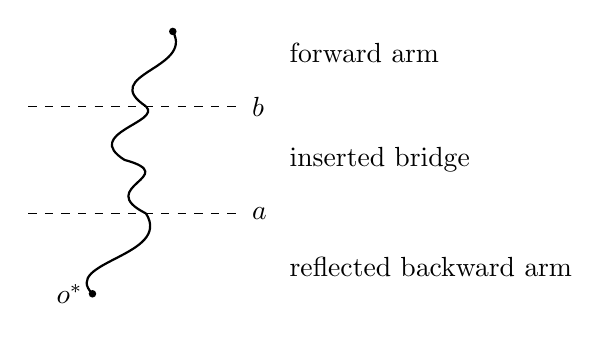
\begin{tikzpicture}[scale=.68]
 \draw[dashed] (-2,2)--(2,2) node[right] {$a$};
 \draw[dashed] (-2,4)--(2,4) node[right] {$b$};
 \draw[thick] (-.8,.5) .. controls (-1.4,1.1) and (.7,1.2) .. (.2,2);
 \draw[thick] (.2,2) .. controls (-.8,2.5) and (.9,2.7) .. (-.2,3)
             .. controls (-1,3.5) and (.5,3.7) .. (.2,4);
 \draw[thick] (.2,4) .. controls (-.7,4.6) and (1.1,4.7) .. (.7,5.4);
 \fill (-.8,.5) circle (2pt) node[left] {$o^*$};
 \fill (.7,5.4) circle (2pt);
 \node[anchor=west] at (2.7,1) {reflected backward arm};
 \node[anchor=west] at (2.7,3) {inserted bridge};
 \node[anchor=west] at (2.7,5) {forward arm};
\end{tikzpicture}
\caption{One insertion, with joining levels $a<b$. Cutting at these
levels and undoing the lower reflection recovers the input up to a
bounded local record. The drawing suppresses the modifications at the
ports.}
\label{R:alt:g:insertion-figure}
\end{figure}

\begin{lemma}[Insertion multiplicities]\label{R:alt:g:multiplicity}
Suppose $h\to\infty$ and $h/H\to0$. Let $\mathcal A_D$ be the walks
rooted at $o$ with diameter at most $h$. Every fixed integer $k\ge1$
satisfies
\begin{equation}\label{R:alt:g:diameter-moment}
 \sum_\omega\rho^{\ell(\omega)}M_{\mathcal A_D}(\omega)^k
       \le C_k H^{C+o_k(1)}h^{k\beta}.
\end{equation}
For fixed $K>0$, let $\mathcal A_E$ be the walks rooted at $o$ of length
at most $H^K$ and absolute vertical endpoint difference at most $h$.
Then
\begin{equation}\label{R:alt:g:endpoint-moment}
 \sum_\omega\rho^{\ell(\omega)}M_{\mathcal A_E}(\omega)^k
 \le C_{k,K}H^{C_K+o_k(1)}
             \{h^\beta(H/h)^{2\beta-1}\}^{k}.
\end{equation}
The sums run over outputs rooted at $o^*$. The exponents $C,C_K$ are
independent of $k$.
\end{lemma}
\begin{proof}
Write $M=M_{\mathcal A}$ for either input class and expand $M^k$ into
ordered $k$-tuples of representations of the same output. We first
locate their seams. Let $z_0,z_f$ be the vertical coordinates of the
output endpoints. Undoing the lower reflection sends the root to height
$2a-z_0$, while removing the inserted height sends the other endpoint to
$z_f-(b-a)$, up to bounded local changes. The original endpoint difference
is therefore $z_0+z_f-a-b+O(1)$. Both input classes satisfy
\begin{equation}\label{R:alt:g:seam-sum}
 |a+b-z_0-z_f|\le C_2h,\qquad H\le b-a\le2H.
\end{equation}
All heights here are in row units, with fixed conversion factors absorbed
in $C_2$.

Put $S=z_0+z_f$ and $E=C_2h$. The possible seams lie in the intervals
\[
 a\in\left[\frac{S-E-2H}{2},\frac{S+E-H}{2}\right],\qquad
 b\in\left[\frac{S-E+H}{2},\frac{S+E+2H}{2}\right].
\]
Every upper seam thus exceeds every lower seam by at least $H-E>0$
for large $H$. Sort the lower seams increasingly and the upper seams
decreasingly:
\[
 a_1\le\cdots\le a_k<b_k\le\cdots\le b_1.
\]
Record ties and the original representation pairing by a permutation
$\pi$: the representation with lower seam $a_i$ has upper seam
$b_{\pi(i)}$. These records cost a factor depending only on $k$.

Every positive gap between consecutive seams in either group is a strict
bridge. The two exterior portions and the portion between $a_k$ and $b_k$
are the only three portions left over. In the diameter case the whole
output lies in a box of side $O(H)$; in the endpoint case it lies in a box
of side $O(H+H^K)$. Fixing the output endpoint and the four extreme seam
ports costs a polynomial in $H$ whose exponent is independent of $k$.
The full-box susceptibility bound then sums the three leftover portions
at cost $H^C$ or $H^{C_K}$. Internal joining ports introduce no additional
position sums: once the relative gap shapes are specified, each has a
unique translation to its joining port.

For the remaining gaps, use heights
\[
 s_1=t_1=0,\qquad
 s_i=a_i-a_{i-1},\quad t_i=b_{i-1}-b_i\quad(2\le i\le k).
\]
The zero slots account for the two extreme seams. Repeated seams give
further zero gaps, with bounded weight. The lower gap of height $s_i$
ends at $a_i$, and the upper gap of height $t_j$ starts at $b_j$.
Consequently the original representation $i$ pairs the slots
$(s_i,t_{\pi(i)})$. Every positive gap appears in exactly one such pair.
Figure~\ref{R:alt:g:pairings-figure} distinguishes this pairing from the
rank pairing used later to sum endpoint constraints.

\begin{figure}[ht]
\centering
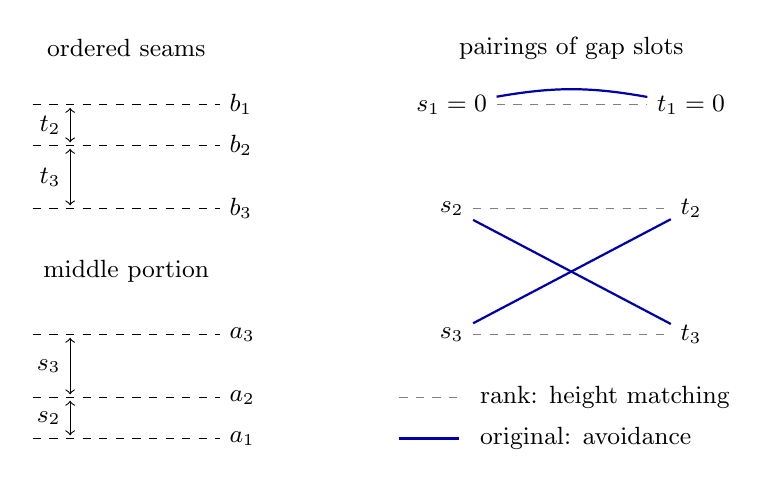
\begin{tikzpicture}[x=.95cm,y=.8cm,font=\small]
 \node at (1.25,6.2) {ordered seams};
 \draw[dashed] (0,0)--(2.5,0) node[right] {$a_1$};
 \draw[dashed] (0,.65)--(2.5,.65) node[right] {$a_2$};
 \draw[dashed] (0,1.65)--(2.5,1.65) node[right] {$a_3$};
 \draw[dashed] (0,3.65)--(2.5,3.65) node[right] {$b_3$};
 \draw[dashed] (0,4.65)--(2.5,4.65) node[right] {$b_2$};
 \draw[dashed] (0,5.3)--(2.5,5.3) node[right] {$b_1$};
 \draw[<->] (.5,.05)--(.5,.60) node[midway,left] {$s_2$};
 \draw[<->] (.5,.70)--(.5,1.60) node[midway,left] {$s_3$};
 \draw[<->] (.5,3.70)--(.5,4.60) node[midway,left] {$t_3$};
 \draw[<->] (.5,4.70)--(.5,5.25) node[midway,left] {$t_2$};
 \node at (1.25,2.65) {middle portion};
 \node at (7.2,6.2) {pairings of gap slots};
 \node (s1) at (5.6,5.3) {$s_1=0$};
 \node (s2) at (5.6,3.65) {$s_2$};
 \node (s3) at (5.6,1.65) {$s_3$};
 \node (t1) at (8.8,5.3) {$t_1=0$};
 \node (t2) at (8.8,3.65) {$t_2$};
 \node (t3) at (8.8,1.65) {$t_3$};
 \draw[dashed,gray] (s1)--(t1);
 \draw[dashed,gray] (s2)--(t2);
 \draw[dashed,gray] (s3)--(t3);
 \draw[thick,blue!65!black] (s1) to[bend left=10] (t1);
 \draw[thick,blue!65!black] (s2)--(t3);
 \draw[thick,blue!65!black] (s3)--(t2);
 \draw[dashed,gray] (4.9,.65)--(5.7,.65);
 \node[anchor=west] at (5.85,.65) {rank: height matching};
 \draw[thick,blue!65!black] (4.9,0)--(5.7,0);
 \node[anchor=west] at (5.85,0) {original: avoidance};
\end{tikzpicture}
\caption{Three representations of one output. The left panel shows the
seam order and the positive gaps; the two extreme slots have height zero.
The right panel illustrates the original permutation
$\pi(1)=1$, $\pi(2)=3$, $\pi(3)=2$. Rank pairs constrain the two gap
heights; original pairs inherit avoidance from an input walk. Connecting
lines in the right panel match variables and do not represent walk
segments. The diagram is not to scale.}
\label{R:alt:g:pairings-figure}
\end{figure}

\paragraph{The diameter class.}
All its gap heights are $O(h)$: each lower seam is within $O(h)$ of
the root height, and each upper seam is within $O(h)$ of the final
height. Put the two gap heights in an original pair into dyadic bins
of scales $\sigma,\tau\le Ch$, with scale one for absent or bounded
gaps. The total bridge mass in a bin of scale $\sigma$ is at most
$C\sigma^\beta$, by \eqref{R:alt:g:strip}.

For two large gaps in an original pair, reverse and reflect the lower
one from its upper endpoint. The two resulting pieces are initial
portions of the input arms at its minimum and avoid one another after
their common first vertex. Move one start to the adjacent port and pass
through the neighboring upward triangle to the same first upper
neighbor. If that triangle was already visited, strictness at the lower
wall forces the visit immediately after the first upper neighbor;
start there and delete the short initial segment. The other arm cannot
use that triangle because it would also use the same upper neighbor.
This recoding has bounded inverse ambiguity and preserves avoidance
through first visits to height $q=c\min(\sigma,\tau)$, for a fixed small
$c>0$. Thus it gives the adjacent-port event in
\eqref{R:alt:g:avoidance}.

Expose each gap from its assigned end through its first renewal at or
above $q$. If the exposed height is $u$, the remaining critical mass
at terminal height $v$ is $B_{v-u}$, with $B_j=0$ for $j<0$. Uniformly
in the exposed shape,
\[
 \sum_{v\le C\sigma}B_{v-u}\le C\sigma^\beta.
\]
The exposed strings have the independent renewal probability law.
After integrating the completions, the paired integral is therefore at
most
\[
 C\sigma^\beta\tau^\beta\min(\sigma,\tau)^{-\beta}H^{o(1)}
 =C\max(\sigma,\tau)^\beta H^{o(1)}
 \le Ch^\beta H^{o(1)}.
\]
If one gap is absent or bounded, the ordinary mass bound for the other
proves the same estimate. Normalize every gap at its assigned test end
and drop all other intersection restrictions. The pairs
$(s_i,t_{\pi(i)})$ use disjoint gap variables, so their bounds multiply
by Tonelli's theorem. The $(1+\log H)^{O(k)}$ dyadic choices contribute
$H^{o_k(1)}$. Together with the three leftover portions, this proves
\eqref{R:alt:g:diameter-moment}.

\paragraph{The endpoint class.}
Its gaps can have height of order $H$, but their rank pairing retains a
constraint. The original pairs satisfy
$|a_i+b_{\pi(i)}-S|\le E$. Two ordered multisets admitting a matching
within $E$ also admit the monotone matching within $E$. Applied to
$a_i$ and $S-b_j$, this gives
\[
 |a_i+b_i-S|\le E,\qquad |s_i-t_i|\le2E\quad(2\le i\le k).
\]
We use these rank pairs to integrate the completion heights, while
keeping $\pi$ for the subsequent avoidance tests.

For a gap in a dyadic bin of scale $\sigma$, put
$w_\sigma=\min(h,\sigma)$ and expose its renewal string through height
$c w_\sigma$, using threshold zero for a bounded gap. Condition on
all exposed strings. A rank pair with one height $O(h)$ has both
heights $O(h)$ and completion mass at most
$Cw_\sigma^\beta w_\tau^\beta$. For a rank pair at comparable scales
$r,r'\gg h$, uniformly in the exposed heights $u_0,v_0$, the completion
mass is at most
\begin{align*}
 &\sum_{\substack{u\asymp r,\ v\asymp r'\\
                |u-v|\le2E,\ u\ge u_0,\ v\ge v_0}}
         B_{u-u_0}B_{v-v_0}\\
 &\hspace{15mm}\le Chr^{2\beta-1}
 \le Cw_r^\beta w_{r'}^\beta(H/h)^{2\beta-1}.
\end{align*}
For the first inequality fix $u-v$, apply Cauchy--Schwarz to the two
translated sequences, and use
$\sum_{j\le Cr}B_j^2\le Cr^{2\beta-1}$; there are $O(h)$ allowed
differences. Here $2\beta-1=1/2>0$. An exposed string that overshoots
its possible endpoint contributes zero, so the bound is uniform without
an extra overshoot condition.

Integrating all completion variables by rank pairs leaves one factor
$w_\sigma^\beta$ per gap and at most $k$ factors
$(H/h)^{2\beta-1}$. The remaining measure is the product of the
independent stopped-string laws. Regroup them now by their original
pairs $(s_i,t_{\pi(i)})$. Each avoidance test costs
$\min(w_\sigma,w_\tau)^{-\beta}H^{o(1)}$, and hence each original
pair contributes at most
\[
 w_\sigma^\beta w_\tau^\beta
       \min(w_\sigma,w_\tau)^{-\beta}H^{o(1)}
 \le h^\beta H^{o(1)}.
\]
Every string is used once. Multiplying these bounds, summing the dyadic
bins, and restoring the polynomial cost of the three leftover portions
proves \eqref{R:alt:g:endpoint-moment}.
\end{proof}

\subsection{The thermal deduction}

Let $c_m$ count unrestricted $m$-edge walks from a fixed vertex, including
the empty walk, and for $T>1$ set
\[
 x_T=\rho e^{-1/T},\qquad
 Z_T=\sum_{m\ge0}c_mx_T^m,\qquad
 \mathbb P_T^{\mathrm{th}}(\gamma)=Z_T^{-1}x_T^{\ell(\gamma)}.
\]
We also use the diameter clause of \cite[Theorem~1.1]{Geometry2026}:
for every $\eta>0$, every finite $A>0$ and every integer $m\ge1$,
the uniform law on $m$-edge walks satisfies
\begin{equation}\label{R:alt:g:uniform-upper}
 \mathbb P_m\{\operatorname{diam}(\gamma)>m^{3/4+\eta}\}
       \le C_{\eta,A}m^{-A}.
\end{equation}
This is an all-length upper bound; the thermal deduction does not
require an all-length uniform endpoint lower bound.

\begin{proposition}[Thermal stretching by insertion]
\label{R:alt:g:thermal}
Under $\mathbb P_T^{\mathrm{th}}$, as $T\to\infty$,
\[
 \begin{gathered}
 \ell(\gamma)=T^{1+o(1)},\qquad
 \operatorname{diam}(\gamma)=T^{3/4+o(1)},\\
 |\gamma_{\ell(\gamma)}-\gamma_0|=T^{3/4+o(1)}
 \end{gathered}
\]
in probability. Each statement means convergence within every fixed
positive exponent slack.
\end{proposition}
\begin{proof}
Every $m$-edge walk lies in a box of side $O(m)$, so full-box
susceptibility gives $c_m\rho^m\le C(1+m)^C$. In particular $Z_T$ is
finite, $Z_T\ge1$, and for every $\xi>0$,
\begin{equation}\label{R:alt:g:thermal-length-upper}
 \mathbb P_T^{\mathrm{th}}\{\ell(\gamma)>T^{1+\xi}\}
 \le\sum_{m>T^{1+\xi}}C(1+m)^Ce^{-m/T}=o(1).
\end{equation}
We first prove the endpoint lower bound on lengths at most $T^2$.
This restriction loses $o(1)$ probability and permits use of the second
multiplicity estimate.

Fix a small $\zeta>0$ and set
$h=T^{3/4-\zeta}$, $H=T^{3/4-\zeta/2}$, rounding heights to integers.
The critical mass of bridges of height in $[H,2H]$ is comparable to
$H^\beta$. By \eqref{R:alt:g:localization}, choosing the fixed
confinement constant $C_*$ sufficiently large retains a fixed fraction
with diameter at most $C_*H$. The mass of bridges in this height window
with $L(\eta)>T$ is at most $T^{-1}H^{25/12+o(1)}$, by
\eqref{R:alt:g:first}. Its ratio to $H^\beta$ is
$H^{4/3+o(1)}/T=o(1)$. On the remainder,
$x_T^{L(\eta)}\ge e^{-1}\rho^{L(\eta)}$. Thus every input admits
insertions of total $x_T$-mass at least $cH^\beta$.

Let $\mathcal A$ consist of inputs of length at most $T^2$ whose absolute
vertical endpoint difference is at most $h$, and let $V$ be their
$x_T$-mass. Since $T^2\le H^K$ for a fixed sufficiently large $K$,
Lemma~\ref{R:alt:g:multiplicity} applies to $M_{\mathcal A}$. Put
\[
 A_h=h^\beta(H/h)^{2\beta-1}\le H^\beta,
 \qquad Q=A_hH^\delta,
\]
where $\delta>0$ will be chosen small after $\zeta$. For every fixed
integer $k\ge1$, the lemma gives
\begin{align*}
 \sum_{M_{\mathcal A}(\omega)>Q}
       x_T^{\ell(\omega)}M_{\mathcal A}(\omega)
 &\le Q^{1-k}\sum_\omega
       \rho^{\ell(\omega)}M_{\mathcal A}(\omega)^k\\
 &\le C_{k,K}A_hH^{C_K+o_k(1)-\delta(k-1)}.
\end{align*}
Choose $k$ so that $\delta(k-1)>C_K+\beta+1$, and then let
$T\to\infty$. The last expression is $o(1)$. This order is possible
because $C_K$ is independent of $k$.

Sum all insertions of inputs in $\mathcal A$. For outputs with
$M_{\mathcal A}\le Q$, there are at most $Q$ representations per
output. Their unrestricted partition sum, rooted at $o^*$, equals
$Z_T$ by the root symmetry established above. The preceding estimate
handles the remaining outputs. Recoverability and the bounded weight
factors therefore give
\begin{equation}\label{R:alt:g:insertion-mass}
 cH^\beta V\le C A_hH^\delta Z_T+o(1).
\end{equation}
Divide by $H^\beta Z_T$ and use
\[
 \frac{A_h}{H^\beta}=(h/H)^{1-\beta}.
\]
For sufficiently small $\delta$, the bound
$V/Z_T\le C(h/H)^{1-\beta}H^\delta+o(1)$ tends to zero. Adding the
discarded length tail proves that the absolute vertical endpoint
difference exceeds $T^{3/4-\zeta}$ with probability tending to one.
The Euclidean endpoint distance has the same lower exponent after
absorbing the fixed row-spacing factor into the slack.

It remains to obtain the diameter upper bound and the length lower
bound. Conditioned on its length, the thermal law is uniform. Fix
$\varepsilon>0$ and choose $\eta,\xi>0$ so that
\[
 (1+\xi)(3/4+\eta)<3/4+\varepsilon.
\]
For $m<T^{1/2}$ the diameter is deterministically at most $CT^{1/2}$.
For $T^{1/2}\le m\le T^{1+\xi}$, the probability of violating
$D\le T^{3/4+\varepsilon}$ is, by
\eqref{R:alt:g:uniform-upper}, at most
$C_{\eta,A}T^{-A/2}$ under each conditional length law. The remaining
lengths have probability $o(1)$ by
\eqref{R:alt:g:thermal-length-upper}. This proves the upper diameter
exponent, and hence the upper endpoint exponent.

For the lower length bound it suffices to take $0<\xi<1/2$.
Choose $\eta,\zeta>0$ such that
\[
 (1-\xi)(3/4+\eta)<3/4-\zeta,
 \qquad \zeta<1/4.
\]
The typical endpoint lower bound excludes lengths $m<T^{1/2}$
deterministically. For $T^{1/2}\le m<T^{1-\xi}$, it forces
$D>m^{3/4+\eta}$, up to a fixed factor absorbed by the strict exponent
inequality. Equation~\eqref{R:alt:g:uniform-upper} bounds the conditional
probability of this event uniformly by $C_{\eta,A}T^{-A/2}=o(1)$.
Thus $\ell\ge T^{1-\xi}$ with probability tending to one. Together
with the length upper tail and $A\le D$, this proves all three claims.
\end{proof}

\begin{thebibliography}{99}
\bibitem{BeatonEtAl2014} N.~R.~Beaton, M.~Bousquet-M\'elou, J.~de Gier, H.~Duminil-Copin and A.~J.~Guttmann. The critical fugacity for surface adsorption of self-avoiding walks on the honeycomb lattice is $1+\sqrt2$. \emph{Communications in Mathematical Physics} \textbf{326} (2014), no.~3, 727--754. \href{https://doi.org/10.1007/s00220-014-1896-1}{doi:10.1007/s00220-014-1896-1}.

\bibitem{BorgsChayesKingMadras2000} C.~Borgs, J.~T.~Chayes, C.~King and N.~Madras. Anisotropic self-avoiding walks. \emph{Journal of Mathematical Physics} \textbf{41} (2000), 1321--1337. \href{https://doi.org/10.1063/1.533189}{doi:10.1063/1.533189}.

\bibitem{CaravennaDoney2019} F.~Caravenna and R.~Doney. Local large deviations and the strong renewal theorem. \emph{Electronic Journal of Probability} \textbf{24} (2019), paper 72, 1--48. \href{https://doi.org/10.1214/19-EJP319}{doi:10.1214/19-EJP319}.

\bibitem{DCS2012} H.~Duminil-Copin and S.~Smirnov. The connective constant of the honeycomb lattice equals $\sqrt{2+\sqrt2}$. \emph{Annals of Mathematics} \textbf{175} (2012), 1653--1665. \href{https://doi.org/10.4007/annals.2012.175.3.14}{doi:10.4007/annals.2012.175.3.14}.

\bibitem{Dyhr2011} B.~Dyhr, M.~Gilbert, T.~Kennedy, G.~F.~Lawler and S.~Passon. The self-avoiding walk spanning a strip. \emph{Journal of Statistical Physics} \textbf{144} (2011), 1--22. \href{https://doi.org/10.1007/s10955-011-0258-z}{doi:10.1007/s10955-011-0258-z}; \href{https://arxiv.org/abs/1008.4321}{arXiv:1008.4321}.

\bibitem{GarsiaLamperti1962} A.~Garsia and J.~Lamperti. A discrete renewal theorem with infinite mean. \emph{Commentarii Mathematici Helvetici} \textbf{37} (1962), 221--234. \href{https://doi.org/10.1007/BF02566974}{doi:10.1007/BF02566974}.

\bibitem{HammersleyWelsh1962} J.~M.~Hammersley and D.~J.~A.~Welsh. Further results on the rate of convergence to the connective constant of the hypercubical lattice. \emph{Quarterly Journal of Mathematics} \textbf{13} (1962), 108--110. \href{https://doi.org/10.1093/qmath/13.1.108}{doi:10.1093/qmath/13.1.108}.

\bibitem{Ioffe1998} D.~Ioffe. Ornstein--Zernike behaviour and analyticity of shapes for self-avoiding walks on $\mathbb Z^d$. \emph{Markov Processes and Related Fields} \textbf{4} (1998), 323--350.

\bibitem{IoffeVelenik2008} D.~Ioffe and Y.~Velenik. Ballistic phase of self-interacting random walks. In \emph{Analysis and Stochastics of Growth Processes and Interface Models}, Oxford University Press, 2008, 55--80. \href{https://doi.org/10.1093/acprof:oso/9780199239252.003.0003}{doi:10.1093/acprof:oso/9780199239252.003.0003}.

\bibitem{IoffeVelenik2010} D.~Ioffe and Y.~Velenik. The statistical mechanics of stretched polymers. \emph{Brazilian Journal of Probability and Statistics} \textbf{24} (2010), no.~2, 279--299. \href{https://doi.org/10.1214/09-BJPS031}{doi:10.1214/09-BJPS031}.

\bibitem{Kesten1963} H.~Kesten. On the number of self-avoiding walks. \emph{Journal of Mathematical Physics} \textbf{4} (1963), 960--969. \href{https://doi.org/10.1063/1.1704022}{doi:10.1063/1.1704022}.

\bibitem{KrachunPanagiotis2026} D.~Krachun and C.~Panagiotis. Quantitative sub-ballisticity of self-avoiding walk on the hexagonal lattice. \emph{Annals of Probability} \textbf{54} (2026), no.~3, 1109--1125. \href{https://doi.org/10.1214/24-AOP1730}{doi:10.1214/24-AOP1730}; \href{https://arxiv.org/abs/2310.17299}{arXiv:2310.17299}.

\bibitem{LSW2004} G.~F.~Lawler, O.~Schramm and W.~Werner. On the scaling limit of planar self-avoiding walk. In \emph{Fractal Geometry and Applications: A Jubilee of Beno\^it Mandelbrot}, Part~2, Proceedings of Symposia in Pure Mathematics \textbf{72}, American Mathematical Society, 2004, 339--364. \href{https://arxiv.org/abs/math/0204277}{arXiv:math/0204277}.

\bibitem{MadrasSlade1993} N.~Madras and G.~Slade. \emph{The Self-Avoiding Walk}. Birkh\"auser, 1993.

\bibitem{Nienhuis1982} B.~Nienhuis. Exact critical point and critical exponents of $O(n)$ models in two dimensions. \emph{Physical Review Letters} \textbf{49} (1982), no.~15, 1062--1065. \href{https://doi.org/10.1103/PhysRevLett.49.1062}{doi:10.1103/PhysRevLett.49.1062}.

\bibitem{companionA}
OpenAI.
Radial transfer estimates and polygon length laws for honeycomb walks.
OpenAI Math Release preprint
\href{https://github.com/openai/math/blob/main/preprints/Radial-transfer-estimates-and-polygon-length-laws-for-honeycomb-walks-September-26-2026/main.pdf}{OAI:Radial-transfer-estimates-and-polygon-length-laws-for-honeycomb-walks-September-26-2026},
2026.

\bibitem{companionU}
OpenAI.
Uniform marked-polygon estimates and sharp finite bridge moments.
OpenAI Math Release preprint
\href{https://github.com/openai/math/blob/main/preprints/Uniform-marked-polygon-estimates-and-sharp-finite-bridge-moments-September-26-2026/main.pdf}{OAI:Uniform-marked-polygon-estimates-and-sharp-finite-bridge-moments-September-26-2026},
2026. Finite bridge theorem.

\bibitem{compL}
OpenAI.
Cylinder amplitudes and logarithmic bridge-length windows on the honeycomb lattice.
OpenAI Math Release preprint
\href{https://github.com/openai/math/blob/main/preprints/Cylinder-amplitudes-and-logarithmic-bridge-length-windows-on-the-honeycomb-lattice-September-26-2026/main.pdf}{OAI:Cylinder-amplitudes-and-logarithmic-bridge-length-windows-on-the-honeycomb-lattice-September-26-2026},
2026.

\bibitem{Geometry2026}
OpenAI.
Mass and covering exponents for fixed-length honeycomb walks.
OpenAI Math Release preprint
\href{https://github.com/openai/math/blob/main/preprints/Mass-and-covering-exponents-for-fixed-length-honeycomb-walks-September-26-2026/main.pdf}{OAI:Mass-and-covering-exponents-for-fixed-length-honeycomb-walks-September-26-2026},
2026.

\bibitem{Nesting2026}
OpenAI.
Cylinder loop weights and planar nesting.
OpenAI Math Release preprint
\href{https://github.com/openai/math/blob/main/preprints/Cylinder-loop-weights-and-planar-nesting-September-26-2026/main.pdf}{OAI:Cylinder-loop-weights-and-planar-nesting-September-26-2026},
2026.

\bibitem{RenewalDiskCompanion}
OpenAI.
Disk transfer representations and confined bridge mass.
OpenAI Math Release preprint
\href{https://github.com/openai/math/blob/main/preprints/Disk-transfer-representations-and-confined-bridge-mass-September-26-2026/main.pdf}{OAI:Disk-transfer-representations-and-confined-bridge-mass-September-26-2026},
2026.

\bibitem{RenewalSignedCompanion}
OpenAI.
Signed cylinder propagation and marked polygons on the honeycomb lattice.
OpenAI Math Release preprint
\href{https://github.com/openai/math/blob/main/preprints/Signed-cylinder-propagation-and-marked-polygons-on-the-honeycomb-lattice-September-26-2026/main.pdf}{OAI:Signed-cylinder-propagation-and-marked-polygons-on-the-honeycomb-lattice-September-26-2026},
2026.

\bibitem{RenewalVacuumCompanion}
OpenAI.
Polynomial vacuum representations and bridge mass for honeycomb walks.
OpenAI Math Release preprint
\href{https://github.com/openai/math/blob/main/preprints/Polynomial-vacuum-representations-and-bridge-mass-for-honeycomb-walks-September-26-2026/main.pdf}{OAI:Polynomial-vacuum-representations-and-bridge-mass-for-honeycomb-walks-September-26-2026},
2026.

\bibitem{Strip2026}
OpenAI.
Critical strip-crossing mass on the honeycomb lattice.
OpenAI Math Release preprint
\href{https://github.com/openai/math/blob/main/preprints/Critical-strip-crossing-mass-on-the-honeycomb-lattice-September-26-2026/main.pdf}{OAI:Critical-strip-crossing-mass-on-the-honeycomb-lattice-September-26-2026},
2026.

\bibitem{Pincus1976} P.~Pincus. Excluded volume effects and stretched polymer chains. \emph{Macromolecules} \textbf{9} (1976), no.~3, 386--388. \href{https://doi.org/10.1021/ma60051a002}{doi:10.1021/ma60051a002}.

\bibitem{Schilling2016} R.~L.~Schilling. \emph{An introduction to L\'evy and Feller processes}. Lecture notes, 2016, version 2. \href{https://arxiv.org/abs/1603.00251v2}{arXiv:1603.00251v2}.
\end{thebibliography}

\end{document}
